% !BIB TS-program = biber

\RequirePackage[l2tabu,orthodox]{nag}

% TODO: decide if one-sided/two-sided
%\documentclass[headsepline,footsepline,footinclude=false,fontsize=11pt,paper=a4,listof=totoc,bibliography=totoc,BCOR=12mm,DIV=12]{scrbook} % two-sided
\documentclass[headsepline,footsepline,footinclude=false,oneside,fontsize=11pt,paper=a4,listof=totoc,bibliography=totoc]{scrbook} % one-sided

% TODO: change citation style in settings
\PassOptionsToPackage{table,svgnames,dvipsnames}{xcolor}

\usepackage[utf8]{inputenc}
\usepackage[T1]{fontenc}
\usepackage[sc]{mathpazo}
\usepackage[ngerman,american]{babel}
\usepackage[autostyle]{csquotes}
\usepackage[%
  backend=biber,
  url=false,
  style=alphabetic,
  maxnames=4,
  minnames=3,
  maxbibnames=99,
  giveninits,
  uniquename=init]{biblatex} % TODO: adapt citation style
\usepackage{graphicx}
\usepackage{scrhack} % necessary for listings package
\usepackage{listings}
\usepackage{lstautogobble}
\usepackage{tikz}
\usepackage{pgfplots}
\usepackage{pgfplotstable}
\usepackage{booktabs}
\usepackage[final]{microtype}
\usepackage{caption}
\usepackage[printonlyused]{acronym}
\usepackage[hidelinks]{hyperref} % hidelinks removes colored boxes around references and links
\usepackage{parskip}
\AtBeginDocument{%
	\hypersetup{
		pdftitle=\getTitle,
		pdfauthor=\getAuthor,
	}
}
\usepackage{ifthen}

\addto\extrasamerican{
	\def\lstnumberautorefname{Line}
	\def\chapterautorefname{Chapter}
	\def\sectionautorefname{Section}
	\def\subsectionautorefname{Subsection}
	\def\subsubsectionautorefname{Subsubsection}
}

\addto\extrasngerman{
	\def\lstnumberautorefname{Zeile}
}

% Themes
\ifthenelse{\equal{\detokenize{dark}}{\jobname}}{%
  % Dark theme
  \newcommand{\bg}{black} % background
  \newcommand{\fg}{white} % foreground
  \usepackage[pagecolor=\bg]{pagecolor}
  \color{\fg}
}{%
  % Light theme
  \newcommand{\bg}{white} % background
  \newcommand{\fg}{black} % foreground
}

\bibliography{bibliography}

\setkomafont{disposition}{\normalfont\bfseries} % use serif font for headings
\linespread{1.05} % adjust line spread for mathpazo font

% Add table of contents to PDF bookmarks
\BeforeTOCHead[toc]{{\cleardoublepage\pdfbookmark[0]{\contentsname}{toc}}}

% Define TUM corporate design colors
% Taken from http://portal.mytum.de/corporatedesign/index_print/vorlagen/index_farben
\definecolor{TUMBlue}{HTML}{0065BD}
\definecolor{TUMSecondaryBlue}{HTML}{005293}
\definecolor{TUMSecondaryBlue2}{HTML}{003359}
\definecolor{TUMBlack}{HTML}{000000}
\definecolor{TUMWhite}{HTML}{FFFFFF}
\definecolor{TUMDarkGray}{HTML}{333333}
\definecolor{TUMGray}{HTML}{808080}
\definecolor{TUMLightGray}{HTML}{CCCCC6}
\definecolor{TUMAccentGray}{HTML}{DAD7CB}
\definecolor{TUMAccentOrange}{HTML}{E37222}
\definecolor{TUMAccentGreen}{HTML}{A2AD00}
\definecolor{TUMAccentLightBlue}{HTML}{98C6EA}
\definecolor{TUMAccentBlue}{HTML}{64A0C8}

% Settings for pgfplots
\pgfplotsset{compat=newest}
\pgfplotsset{
  % For available color names, see http://www.latextemplates.com/svgnames-colors
  cycle list={TUMBlue\\TUMAccentOrange\\TUMAccentGreen\\TUMSecondaryBlue2\\TUMDarkGray\\},
}

% Settings for lstlistings
\lstset{%
  basicstyle=\ttfamily,
  columns=fullflexible,
  autogobble,
  keywordstyle=\bfseries\color{TUMBlue},
  stringstyle=\color{TUMAccentGreen},
  captionpos=b
}


% TODO: change thesis information
\newcommand*{\getUniversity}{Technische Universität München}
\newcommand*{\getFaculty}{Informatics}
\newcommand*{\getDegree}{Information Systems}
\newcommand*{\getSchool}{Computation, Information and Technology}
\newcommand*{\getTitle}{Visualisation and statistical analysis of performance measurements of database systems}
\newcommand*{\getTitleGer}{Visualisierung und statistische Aufbereitung von Performance Messungen von Datenbanksystemen}
\newcommand*{\getAuthor}{Julian Macias De La Rosa}
\newcommand*{\getDoctype}{Master's Thesis}
\newcommand*{\getSupervisor}{Prof. Thomas Neumann}
\newcommand*{\getAdvisor}{Maximilian Bandle}
\newcommand*{\getSubmissionDate}{20.10.2023}
\newcommand*{\getSubmissionLocation}{Munich}

\usepackage{graphicx}

\begin{document}

% Set page numbering to avoid "destination with the same identifier has been already used" warning for cover page.
% (see https://en.wikibooks.org/wiki/LaTeX/Hyperlinks#Problems_with_Links_and_Pages).
\pagenumbering{alph}
\begin{titlepage}
  % HACK for two-sided documents: ignore binding correction for cover page.
  % Adapted from Markus Kohm's KOMA-Script titlepage=firstiscover handling.
  % See http://mirrors.ctan.org/macros/latex/contrib/koma-script/scrkernel-title.dtx,
  % \maketitle macro.
  \oddsidemargin=\evensidemargin\relax
  \textwidth=\dimexpr\paperwidth-2\evensidemargin-2in\relax
  \hsize=\textwidth\relax

  \centering

  \IfFileExists{logos/tum-logo.pdf}{%
    \includegraphics[height=20mm]{logos/tum-logo.pdf}
  }{%
    \vspace*{20mm}
  }

  \vspace{5mm}
  {\huge\MakeUppercase{School of \getSchool{} --- \getFaculty{}} \par}

  \vspace{5mm}
  {\large\MakeUppercase{\getUniversity{}} \par}

  \vspace{15mm}
  {\Large \getDoctype{} in \getDegree{} \par}

  \vspace{10mm}
  {\huge\bfseries \getTitle{} \par}

  \vspace{10mm}
  {\LARGE \getAuthor{}}

  \IfFileExists{logos/faculty-\fg.pdf}{%
    \vfill{}
    \includegraphics[height=20mm]{logos/faculty-\fg.pdf}
  }{}
\end{titlepage}


\frontmatter{}

\input{pages/title}
\input{pages/disclaimer}
\addcontentsline{toc}{chapter}{Acknowledgments}
\thispagestyle{empty}

\vspace*{20mm}

\begin{center}
    {\usekomafont{sectioning}\usekomafont{section} Acknowledgments}
\end{center}

\vspace{10mm}

I extend my sincere gratitude to my advisor Maximilian Bandle for his invaluable guidance and unwavering support throughout this research journey. His prompt responses and willingness to assist at any time significantly enriched the quality of this work.

I would also like to express my appreciation to Tom Papke for his generous assistance during the integration process of the Query Plan Visualizer. His expertise and collaborative spirit played a crucial role in enhancing the functionality of the Benchy Viewer.

This research would not have been possible without the encouragement and support of these individuals, and I am truly thankful for their contributions to the successful completion of this thesis.

\cleardoublepage{}

\chapter{\abstractname}

\begin{figure}[h]
    \centering
    \begin{subfigure}[b]{0.3\linewidth}
      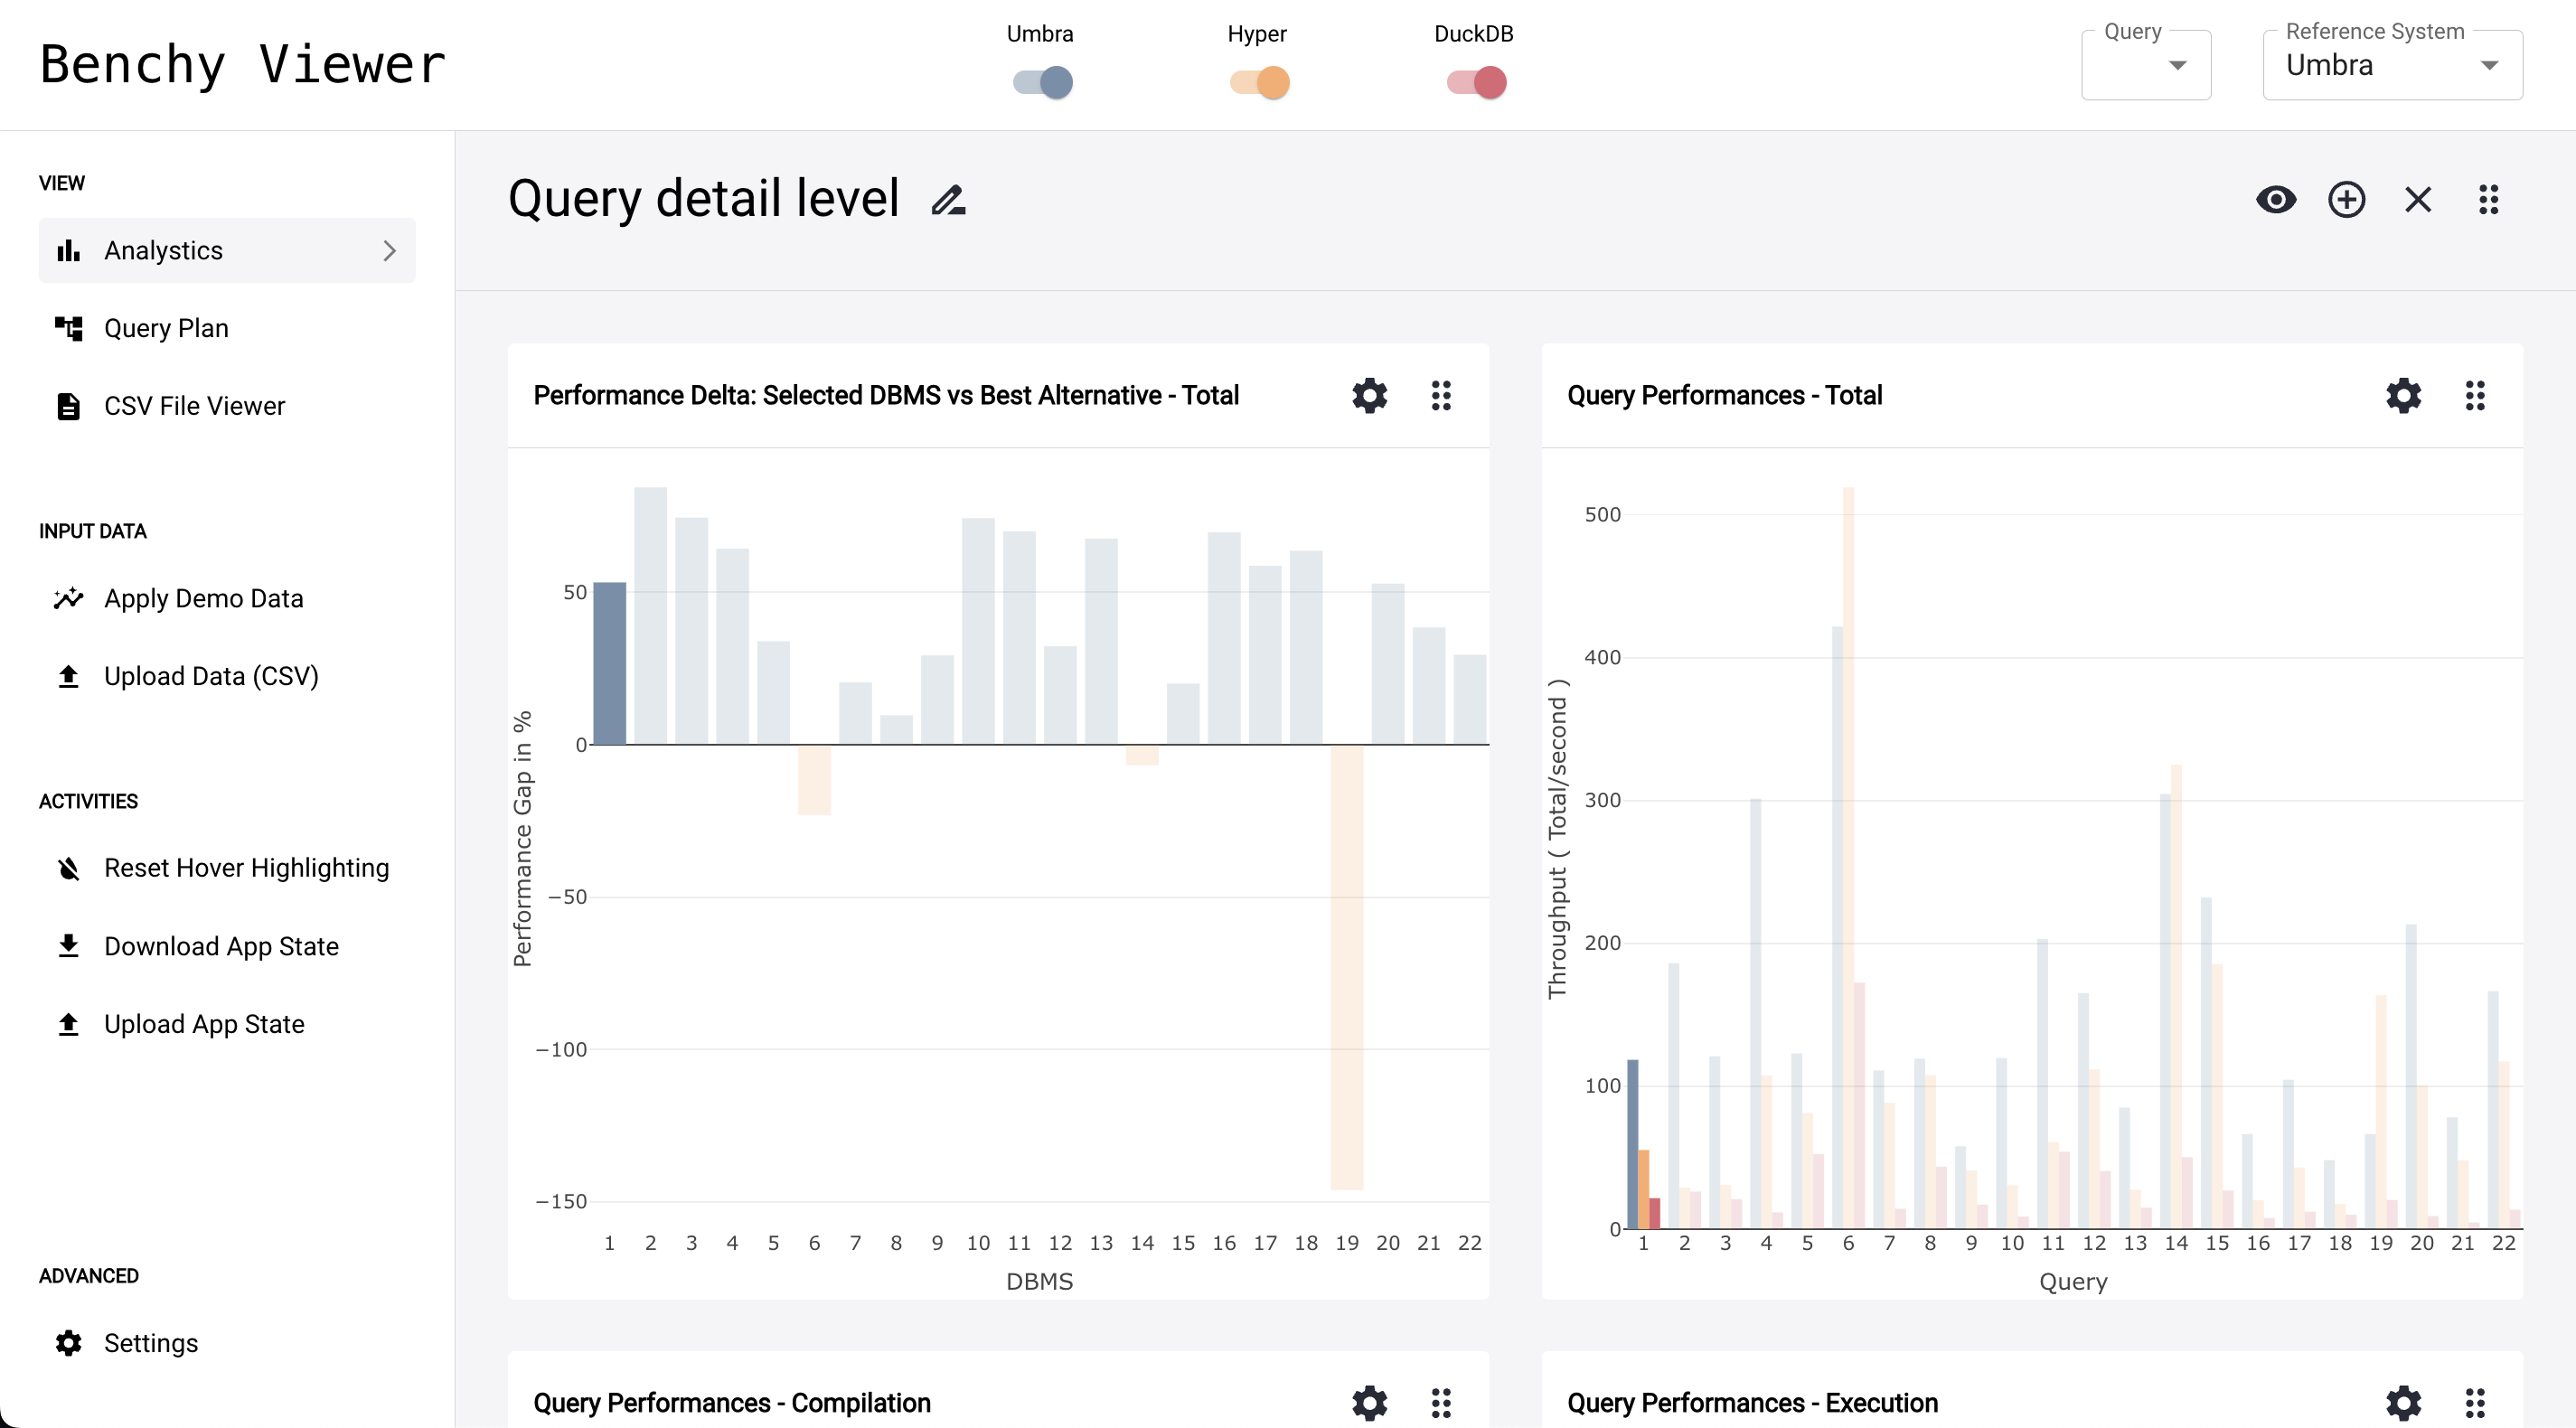
\includegraphics[width=\linewidth]{figures/app.png}
      \caption{Analytics Dashboard.}
        \label{fig:abstract-page}
    \end{subfigure}
    \hspace{0.5cm} % Adjust the horizontal space between the figures
    \begin{subfigure}[b]{0.3\linewidth}
      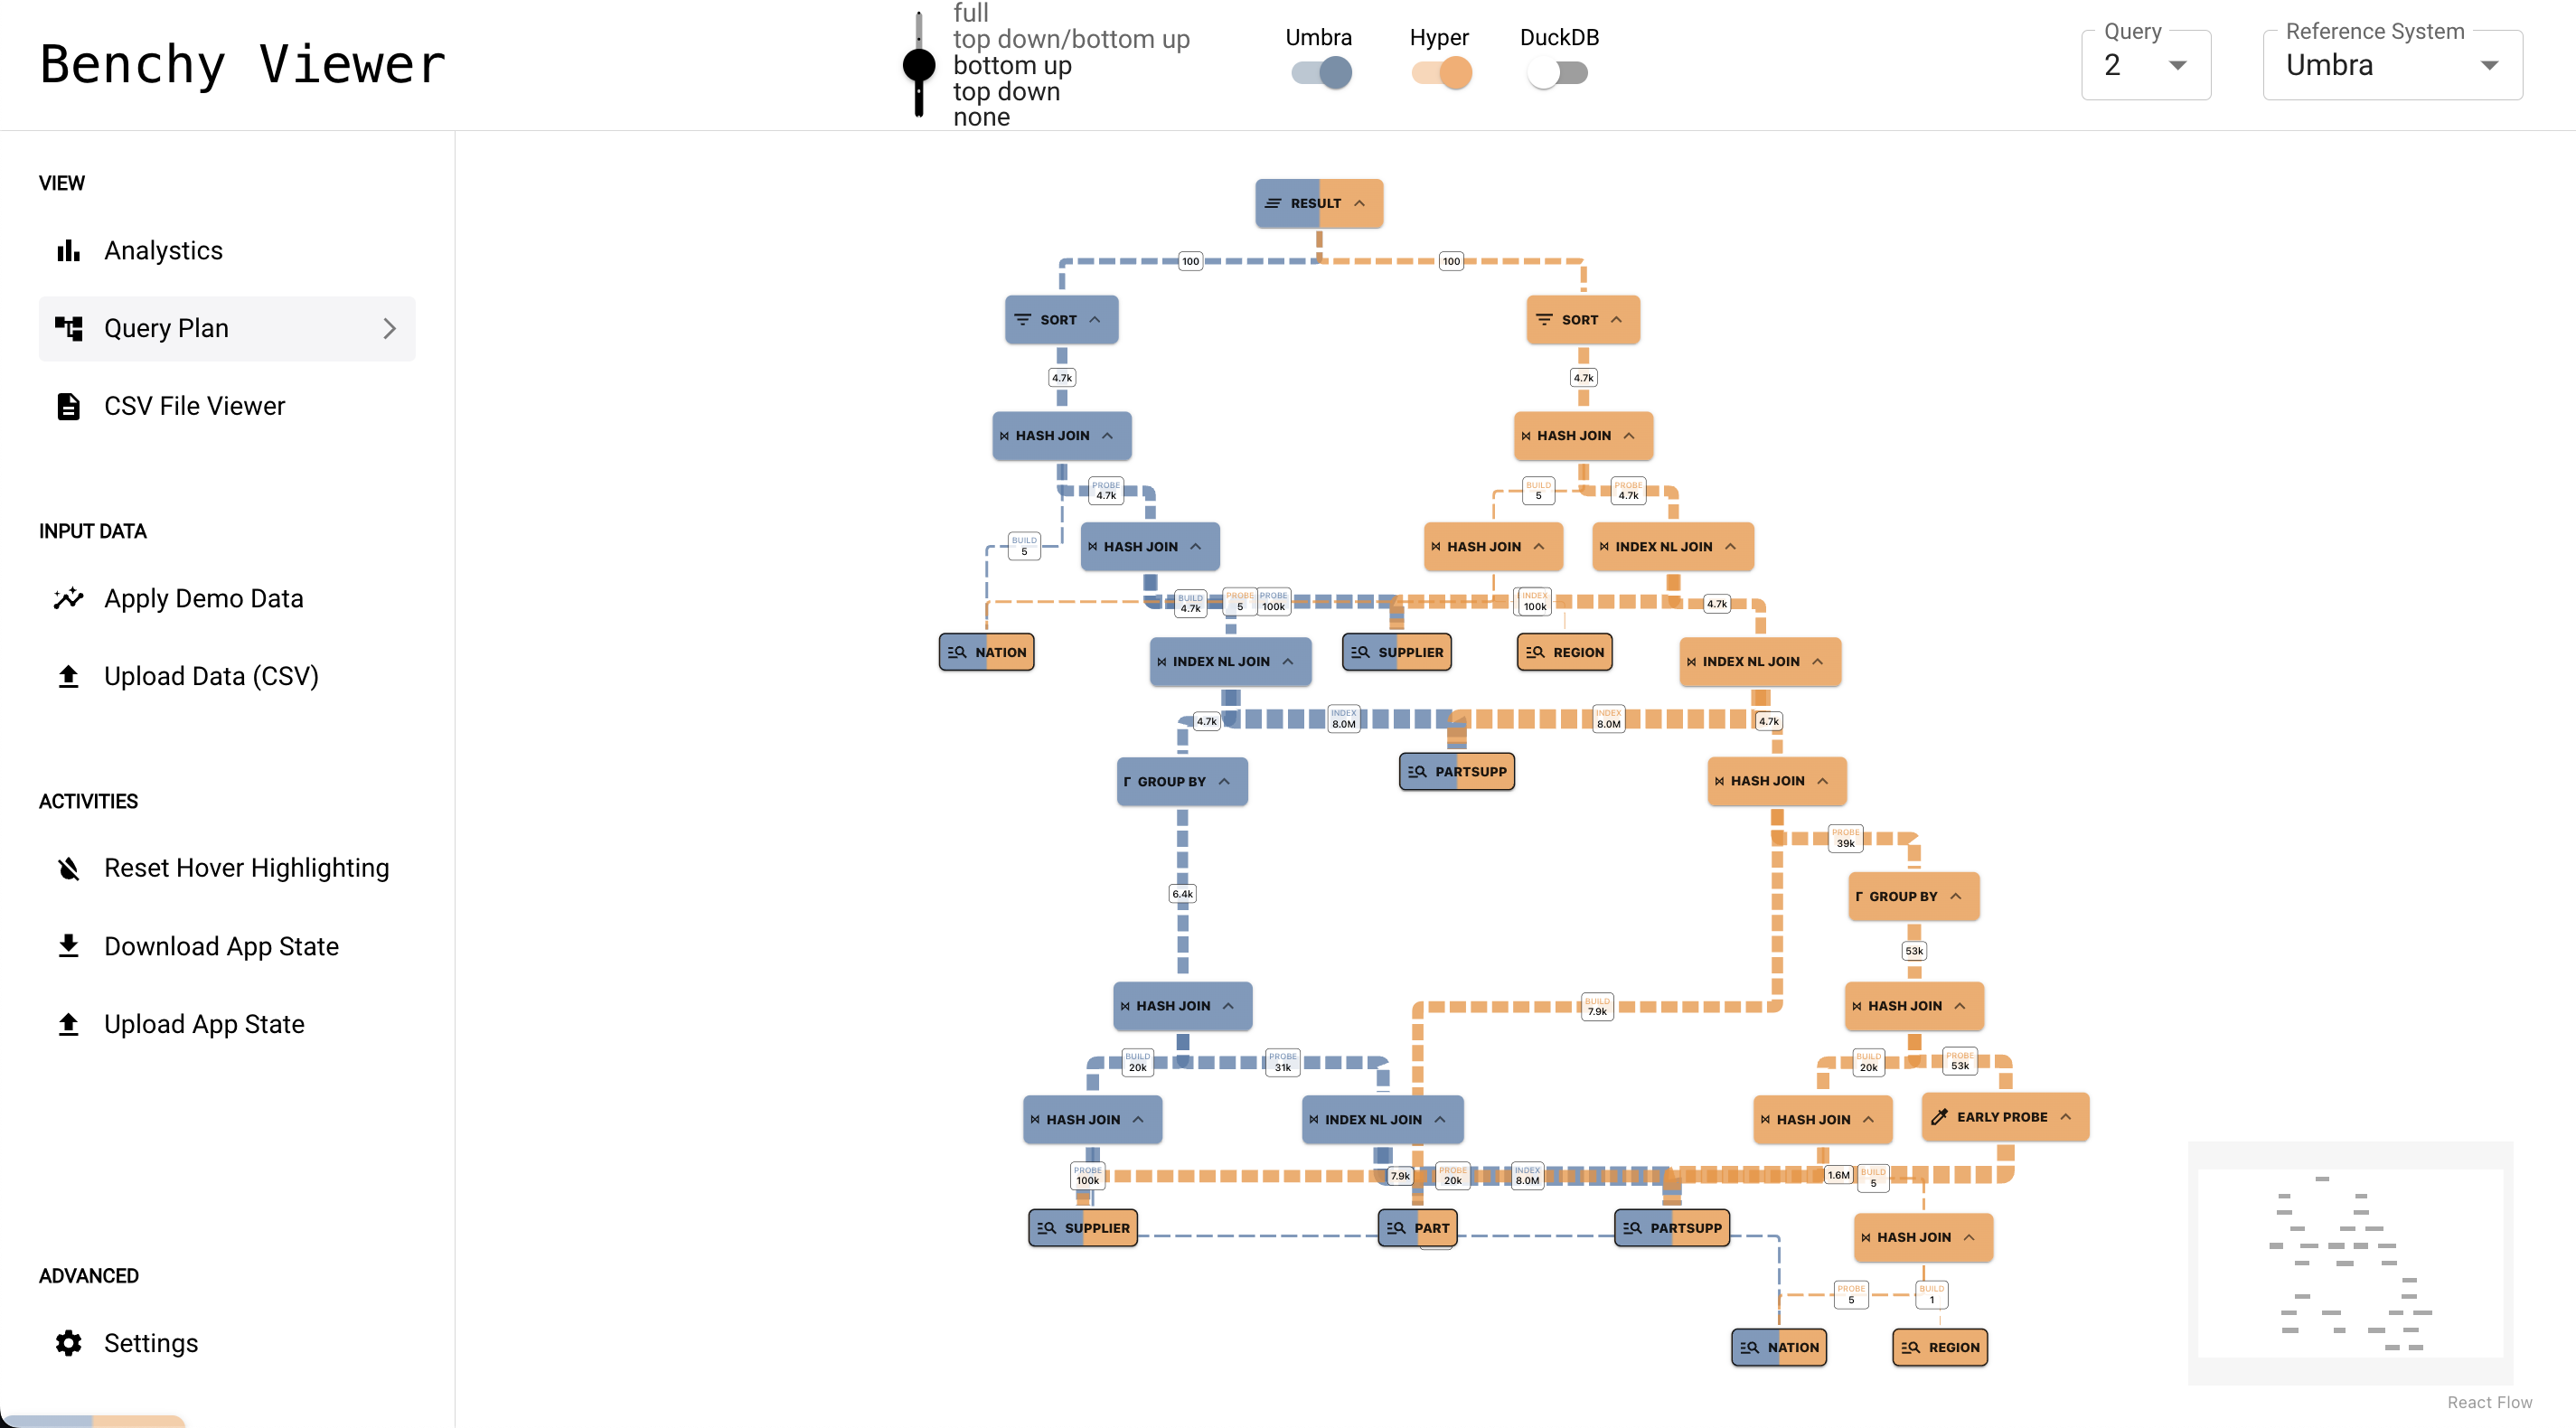
\includegraphics[width=\linewidth]{figures/app-query-plan.png}
      \caption{Query Plan View.}
        \label{fig:abstract-query-plan}
    \end{subfigure}
    \hspace{0.5cm} % Adjust the horizontal space between the figures
    \begin{subfigure}[b]{0.3\linewidth}
      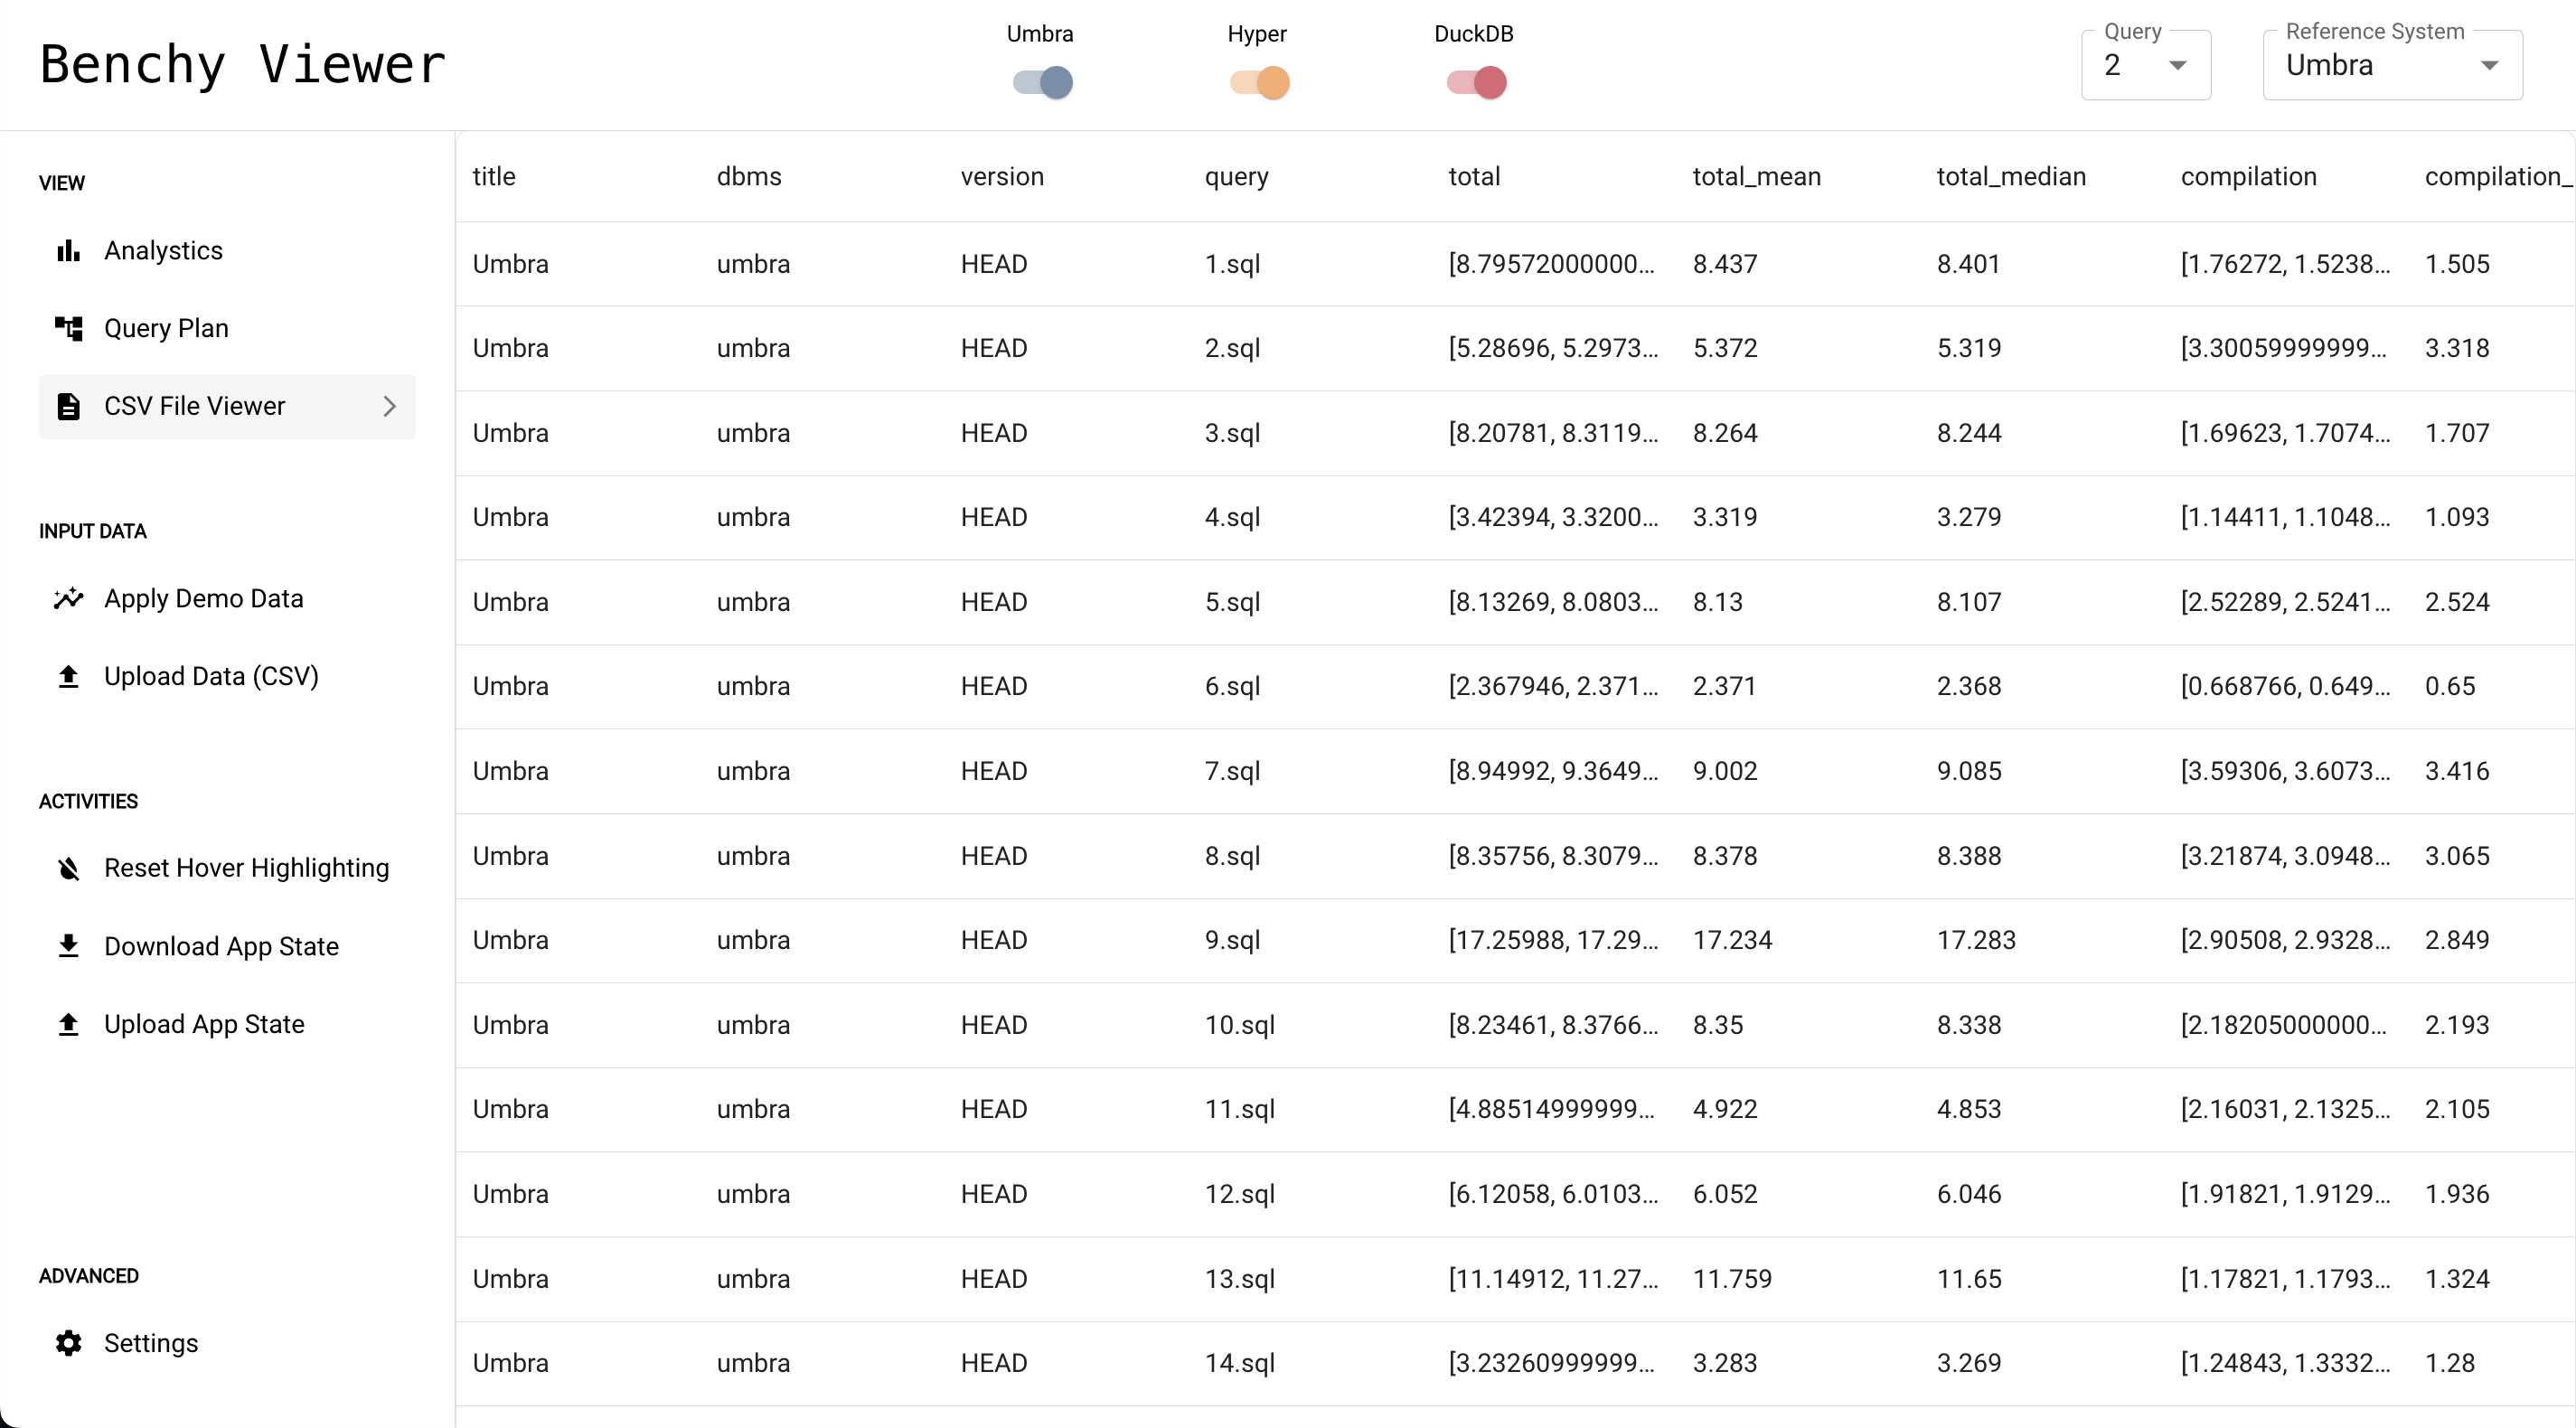
\includegraphics[width=\linewidth]{figures/app-data-viewer.png}
      \caption{Input File Viewer.}
        \label{fig:abstract-data-viewer}
    \end{subfigure}
    \caption{Benchy Viewer: Tool for analyzing performance measurements of database systems through interactive visualizations.}
    \label{fig:abstract}
  \end{figure}

%   In the ever-evolving landscape of database systems,

% This master thesis introduces the Benchy Viewer, a web-based serverless application designed for interactive exploration and analysis of performance data from various database systems. The primary objective is to empower database engineers by providing an intuitive platform for in-depth query execution analysis.\\
% We focus on consolidating a variety of interactive diagrams that portray diverse information content, aiming to elevate the interpretation of profiling data in database systems. The scope delineates the primary questions guiding the investigation, with a focus on the design and development of the Benchy Viewer application, as well as the exploration of statistical methods for analyzing performance data in database systems.


% The thesis structure navigates through related work, theoretical foundations, and the implementation of the Benchy Viewer. It scrutinizes the theoretical underpinnings of database systems, delves into datasets and data structures, and unveils the intricacies of implementation, emphasizing features, interaction capabilities, and design guidelines.

Embarking on the intricate journey of database performance optimization, this thesis underscores the pivotal role of performance analysis in benchmark data. A foundational understanding of system intricacies is paramount for overall performance enhancement. Recognizing the indispensability of visualizations in this analytical process, our work introduces the Benchy Viewer, a web-based serverless application meticulously designed to elevate the analysis of performance benchmark data.

Our main focus is on delivering interactive visualizations through an intuitive user interface, creating an environment where database developers can seamlessly navigate and interpret benchmark data. Developed using React, the Benchy Viewer stands out for its flexibility and the degree of interaction embedded in its intuitive user interface, empowering developers to dynamically explore benchmark data. It offers diverse perspectives, allowing users to view performance metrics from various angles, including a comparison perspective of query plans across different system instances, adding a layer of depth to performance analysis.

Built on an extensible architecture, the Benchy Viewer paves the way for future improvements. Its adaptability enables the incorporation of additional visualizations and analytical perspectives. 
In essence, the Benchy Viewer emerges as a transformative tool, achieving varied perspectives through interactive visualizations and an intuitive user interface, while its extensible architecture opens avenues for continuous enhancement.







\microtypesetup{protrusion=false}
\tableofcontents{}
\microtypesetup{protrusion=true}

\mainmatter{}

% !TeX root = ../main.tex
% Add the above to each chapter to make compiling the PDF easier in some editors.

\chapter{Introduction}\label{chapter:introduction}
Interactive performance visualization is a powerfull skill and plays a vital role for the demonstration of meaningful data insights in the context of performance measurements. Our goal is to use this powerfull skill properly to enable potential optimization possibilities for compiling database systems.

\section{Motivation}
\section{Technical Background}
\subsection{React}
\subsection{Redux}
\subsection{React Sweet State//}
\subsection{Plotly}
\subsection{React-Flow}
\subsection{Material UI}
\section{Existing Visualization of Performance Data of Umbra //PDF }
\section{Research objectives}
\section{Scope and contribution of the thesis}
\section{Thesis structure}


% TODO: add more chapters here 
% !TeX root = ../main.tex
% Add the above to each chapter to make compiling the PDF easier in some editors.

\chapter{Related Work}\label{chapter:relatedWork}
In this chapter, we give an overview about the existing work in the domain of the visualization of database performance profiling.
We will investigate the importance of optimizing query executions in database systems and the role of visualizations in identifying potential improvements.
As performant measurement and analysis play a crucial role in developing and optimizing database systems, 
it is essential to examine the state-of-the-art techniques and tools that have been used in this domain.
We will also cover a visualization tool closely associated with this thesis, as its key feature is integrated into the Benchy Viewer.

\section{Performance Visualization}
Sektion eher in Background
\textcolor{red}{Todo: Was es alles in dieser Domain gibt. Was effektiv ist und wir benutzen. Was wir nicht benutzen  mit Begründung.  }

\section{Database Performance Profiling }

Performance profiling in database systems is crucial for optimizing their execution regarding achieving optimal hardware utilization and query efficiency.
Profiling the performance of database systems involves collecting and analyzing various performance metrics during query execution.
\\Besides profilers presenting results at the instruction and function granularity, a paper on "Profiling Dataflow Systems on Multiple Abstraction Levels" \cite{profiling-dataflow} proposes a solution that tracks the code generation process and aggregates profiling data to higher abstraction levels. This approach helps bridging the semantic gap between low-level profiles and high-level constructs, making it easier for developers to interpret profiling results and identify bottlenecks and hotspots in the system. The paper introduces the concept of Tailored Profiling, which extends the compilation steps to annotate the generated code with metadata. This enables the mapping of profiling results back to desired abstraction levels and provides more understandable profiling data.
Building on the insights from this work, the opportunity arises to create more meaningful visualizations regarding the dataflow in system performance profiling.
\\ An essential concept of this thesis is to build upon the concepts of tailored profiling to gain a deeper understanding of the system's performance and support the location of potential optimization possibilities. Thus, we integrate an intuitive and interactive query plan visualization feature that is able to break down complex queries into their constituent operators and pipelines. We clarify further details about the query plan in section \ref{subsec:semantic-diff} and in chapter X (Implementation) \textcolor{red}{Todo: Chapter linking}.

\section{Related visualization tools}

This section explores related visualization tools that aid developers analyse their database system queries, with a specific focus on performance visualization. We will go through the Query Plan Difference Visualiser and the Umbra Profiler \textcolor{red}{Todo: Zitat}, which are both tools, that are strongly related to the Benchy Viewer. 


\subsection{Query Plan Difference Visualiser}
\label{subsec:semantic-diff}

The efficiency of a database system's query execution relies on the physical execution plan it generates.  Given the complexity of finding the best plan, the comparison of query plans both within a single system and accross different systems has garnered attention. This comparative analysis aims to gain valuable insights and identify potential optimisation opportunities. Previous efforts in this direction have mainly focused on quantitative metrics, in particular the total cost of the plan.
\begin{figure}[h]
    \centering
    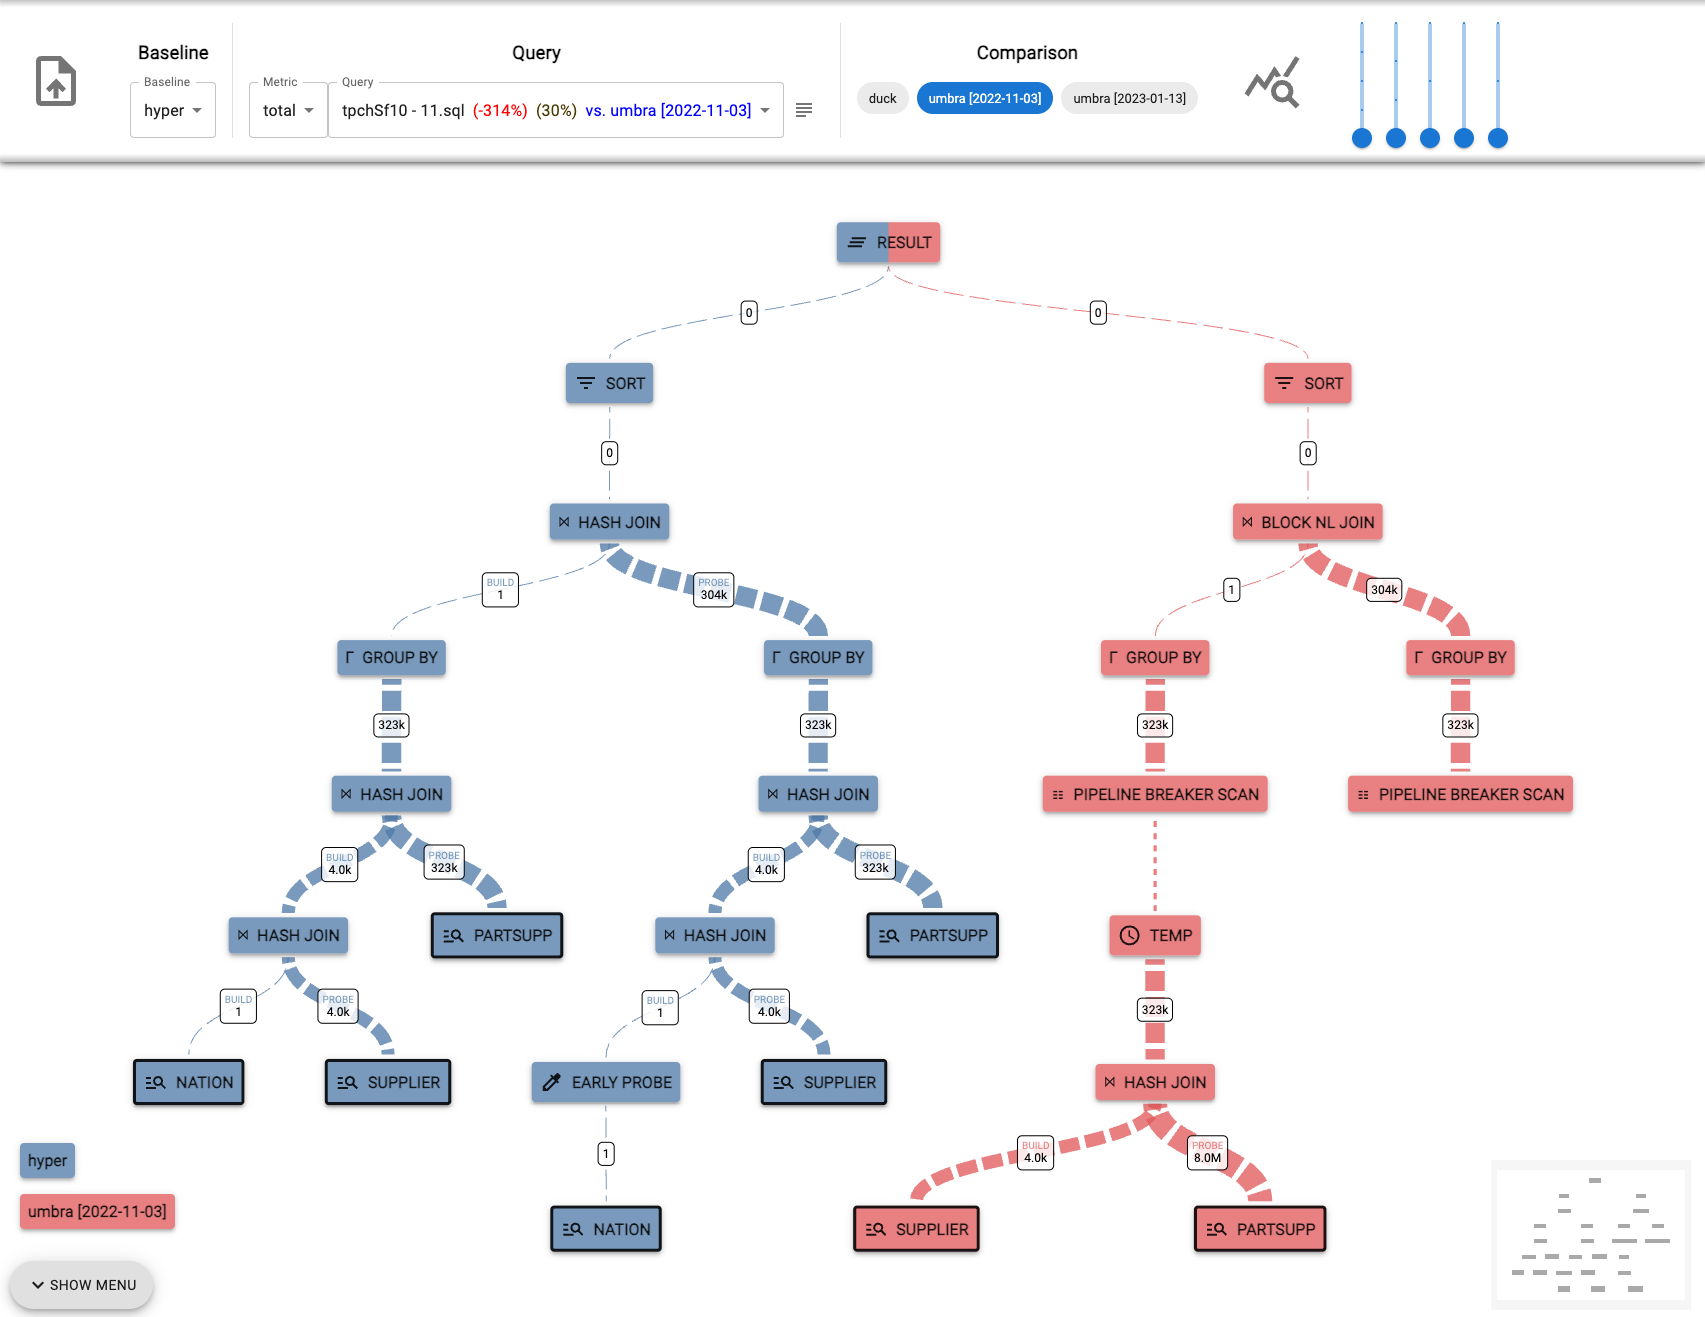
\includegraphics[width=0.8\linewidth]{figures/semantic-diff.png}
    \caption{Query Plan Difference Visualiser}
    \label{fig:semantic-diff}
  \end{figure}

\noindent 
Query execution plans describe the step-by-step hierarchical sequence of physical operations that a database system uses to process a particular SQL query. The fascinating aspect of this is that identical queries can result in different plans when processed by different database systems. This variability in plan generation can have a significant impact on overall performance.
\\The Query Plan Difference Visualiser is a web application that compares and visualises these physical query execution plans from different relational database systems, as shown in Figure~\ref{fig:semantic-diff}. It is designed for database developers who want to inspect the correlation between variations in query execution speed and the respective query plans. Through enhanced hierarchical differencing algorithms with semantic information about query plans, the tool is able to interactively capture and present  the difference between query plans. This is particularly useful for comparing different database systems or different versions of the same system when varying query plans are used by the systems under test to process the same query. Furthermore, it provides the flexibility to pick an arbitrary number of systems for which to compare plans and select a metric for evaluating query performance, such as total runtime or compilation time. For the given metric, it directly shows the difference between the baseline system and the better system.
\\ Once a query plan is initialized, the comparative tool provides the option to improve the clarity of the query plan visualization using various configuration settings. For instance, the tool offers a match mode selection, allowing users to capture the tree from, e.g., a top-down or bottom-up matching perspective. With the Expand and Collapse feature, users can collapse entire subtrees and selectively expand specific child nodes, customizing the focus of the visualization and tailoring the area of attention to the most interesting parts of the tree.
For query plans containing Directed Acyclic Graph (DAG) edges, such as the Pipeline Breaker Scan operator in Umbra, the tool offers support to include these DAG edges and consider them during the matching process. Additionally, to enable more effective comparisons against systems that generate non-DAG-shaped plans, an option is available to replicate subtrees instead.
\\ Database developers often find value in comparing query plans, particularly when they have thoroughly examined different results using quantitative metrics. 
Therefore, we decided to integrate the Query Plan Difference Visualiser with its core features of comparing query plans. In addition to visualising quantitative metrics from different database systems within the Benchy Viewer, the incorporation of the Query Plan Difference Visualiser with its capabillities will further enhance our objective of simplifying the detection of performance bottlenecks in query execution and optimizing database systems.

Hence, the Query Plan Difference Visualiser is strongly related to this thesis and we will dive deeper into the integration of the comparative tool in Chapter X. \textcolor{red}{Todo: Chapter linking}



\subsection{Umbra Profiler}
The Umbra Profiler is a tool that enables in-depth analysis for identifying bottlenecks in query execution processes of the database system Umbra.
\\ It is integrated with a backend application for preparing extensive profiling data and offers multiple perspectives, including a runtime dashboard, a memory dashboard, and an instruction dashboard, each depicting distinct information, as illustrated in Figure~\ref{fig:umbra-profiler}.

\begin{figure}[h]
  \centering
  
\includegraphics[width=1\linewidth]{figures/umbra-profiler.png}
  \caption{Umbra-Profiler: A tool for analyzing and profiling Umbra’s compiling queries. From left-to-right: runtime dashboard, memory dashboard, and instruction dashboard.}
  \label{fig:umbra-profiler}
\end{figure}

\noindent 
The runtime dashboard is the default view that appears after providing recorded hardware samples of a query execution. It offers an initial overview of the query execution structure, allowing users to analyze the activity of specific processor events, operators, and pipelines over time. Abnormalities in execution, such as resource-intensive operations, can be identified, aided by visualizations including key performance indicators, activity histograms, bar charts, query plans, sunburst charts, and swim lanes.
\\The memory behavior dashboard focuses on memory access patterns in query execution. It offers memory heatmaps for each operator, showing either absolute memory accesses or sequential memory address differences.
\\The instruction Dashboard facilitates detailed analysis of query execution using Umbra Intermediate Representation (UIR) \textcolor{red}{Zitat} instructions. It allows comparison of UIR instructions with query plans to identify performance problems based on costs and occurrences. 
\\Similar to the Benchy Viewer, the goal is to support database engineers in optimizing query execution by providing an interactive user interface, enabling an effective in-depth analysis process. 
\\The Umbra Profiler is designed based on the innovative Tailored Profiling approach \cite{profiling-dataflow}, where the connection between query plans and compiled code is maintained. This technique was previously unaddressed by standard profilers and is now used in both the Umbra Profiler and the Benchy Viewer.  
\\However, unlike the Benchy Viewer, the Umbra Profiler is focused to operate exclusively with the database system Umbra. In contrast, the Benchy Viewer has the versatility to function with multiple database systems or multiple instances of a single database system.
\\In broad terms, the Umbra Profiler is primarily designed for in-depth analysis of query performance within a single database system, while the Benchy Viewer is oriented towards its comparative function, enabling the comparison of queries executed by different instances. This comparative approach is the main essence  of the concept of the Benchy Viewer, which aims to enhance the understanding of differences between database instances.

An effective scenario that synergizes the Benchy Viewer and the Umbra Profiler would involve identifying intriguing queries using the Benchy Viewer and subsequently conducting comprehensive analyses using the Umbra Profiler.



% !TeX root = ../main.tex
% Add the above to each chapter to make compiling the PDF easier in some editors.

\chapter{Theoretical Foundations}\label{chapter:theoreticalFoundacions}

In this chapter, we investigate the theoretical foundations by examining database performance measurements and in the next step describing used datasets and the data structure.\\We will start by discussing the characterisitcs of database systems and elaborate on the significance of performance measurements in this context. Additionally, we will outline the common performance metrics, that play a central role in the evaluation of performance analysis.
\\ For clarifying used datasets and the data structure, we commence by describing the utilized performance data, followed by giving an overview of the structure of the Benchy Viewer's input file containing the performance measurements. Moreover, the data prepration for this input file will be explained.

\section{Database Systems and Performance Measurements}
Performance measurement and analysis are fundamental in the realm of database systems. They offer valuable insights into system behavior, helping to pinpoint bottlenecks and optimization opportunities. This process is crucial not only for evaluating one's own system but also for making meaningful comparisons with other systems. Visualisations play a pivotal role in understanding performance data and are often used to convey complex findings effectively.
To interpret performance data effectively, we begin by understanding the characteristics and core traits of a Database System.

\subsection{Characteristics of Database Systems}
Database systems are complex structures that manage and store vast amounts of data efficiently, involving interrelated factors that must be finely tuned to ensure optimal performance.\\
One of the fundamental functions of a database system is query processing. A query is essentially a request for specific information from the database. This involves receiving and then executing that query. The process includes tasks like parsing, optimization, and execution.\\
Queries go through two main phases: compilation and execution. \textcolor{red}{Figure mit Compilation und Execution} During compilation, the query is transformed into an execution plan. This plan outlines the steps the system should take to retrieve the requested data. In the execution phase, the system follows this plan to fetch the data.\\
Query plans are roadmaps that guide how a database executes queries, with operators as specialized components responsible for specific actions. Operators, like selection and join operators, perform data operations during query execution, such as filtering and combining data. Optimizing query plans is vital for database efficiency, with query optimizers selecting the best plan considering factors like data distribution and hardware capabilities.\\
Query processing can be time-consuming due to various challenges. For instance, complex queries, large datasets, and suboptimal query plans can lead to slow performance. Identifying and overcoming these challenges is essential for improving system efficiency.

Understanding these characteristics is key to understanding the complexity of database performance. Challenges such as optimising query plans and dealing with large data sets are common, and manual assessment is often impractical.\\
The need for objective metrics is therefore obvious, making performance measurements essential for targeted optimisations. Due to the complexity of these metrics, visualisation techniques are invaluable for easier interpretation and analysis.\\
In the next section, we will explore the important role of performance measurements and their visualisation in improving database efficiency.


\subsection{Importance of Performance Measurements}
Database systems are the core of a wide range of applications. Consequently, their performance matters not just in terms of user-friendliness and reliability, but also in terms of efficiency. Performance measurements play a central role in this context.\\
One of the key advantages of performance measurements lies in their capacity to assist in optimization efforts. By quantifying performance in a series of metrics, database developers can pinpoint precisely where bottlenecks occur, whether it is in the compilation phase, the query plan, data retrieval, or any other component of the database system. This focused approach minimizes the trial and error often involved in performance tuning and directs resources toward the most impactful modifications.\\
Furthermore, bottlenecks and areas with room for improvement are often not obvious. With the aid of performance measurements, these elements come into sharp focus. Measurements can reveal, for example, if the system's weak point lies in query compilation or if the query plan needs to be optimized. Understanding and interpreting the findings correctly is crucial for making informed decisions on where to prioritize improvement efforts.\\
Another fundamental aspect is scalability. In a world where data is continuously growing, the scalability of a database system becomes a certain priority, because data volumes continue to grow. Performance measurements can identify the limitations of a system as it scales, revealing performance degradation points before they become critical bottlenecks. This approach is not only applied to solve current needs of data volume, but is also contributing to the system's scalability for the future.\\
Referring back to the introduction's implication, the complexity of performance metrics can often be overwhelming. Visualisation techniques become invaluable tools in this context. By translating numerical data into graphical elements, these visualisations can illuminate patterns and trends that could otherwise be easily overlooked, offering an intuitive and interactive way to understand the performance bottlenecks and operational nuances.

In summary, performance measurements are essential in the effective management and optimization of complex database systems. With these basic principles in mind, the next section examines common performance metrics for evaluating database systems, which serve as the quantitative backbone for the analyses and visualisations discussed here.

\subsection{Common Performance Metrics}
Understanding the importance of performance measurements in database systems necessitates a deeper dive into the specific metrics that help analyse various aspects of performance. This section explores effective metrics and how they are used within this domain, which indicates the desired functionalities of the Benchy Viewer in terms of interaction and visualisation.\\
In the paper "Bringing Compiling Databases to RISC Architectures" \cite{Bringin-Compiling-Databases-to-RISC} the compilation performance of the dominant x86-64 server architecture is contrasted  with the new introduced code generator designed for AArch64-based systems. This is interesting for the Benchy Viewer as it conducts a comparative analysis of different perspectives in terms of performance,  leveraging specific performance metrics that are also visually represented.\\ 
The paper utilizes both quantitative and subjective performance metrics when addressing the query compilation strategy. However, for the scope of our visualisation, we focus on the quantitative metrics. Relying on quantitative metrics allows for clear, objective visualisation that can represent performance differences, whereas subjective metrics does not offer the same level of clarity and consistency in a visual representation.\\
Here one of the most central metrics is the throughput, a key metric in databases, measures the number of processed tuples per second and is a primary optimization target. In the context of compiling databases, throughput is primarily influenced by the quality of the generated machine code for queries.\\
Another fundamental metric is the latency, which is the time needed for generating and compiling query code before execution, with lower latency being particularly important for real-time transactional systems.\\
With these two metrics, the paper shows an intuitive and clear overview of how different database instances perform on the TPC-H benchmark, as demonstrated in Figure~\ref{fig:risc-metrics}.

\begin{figure}[h]
  \centering
  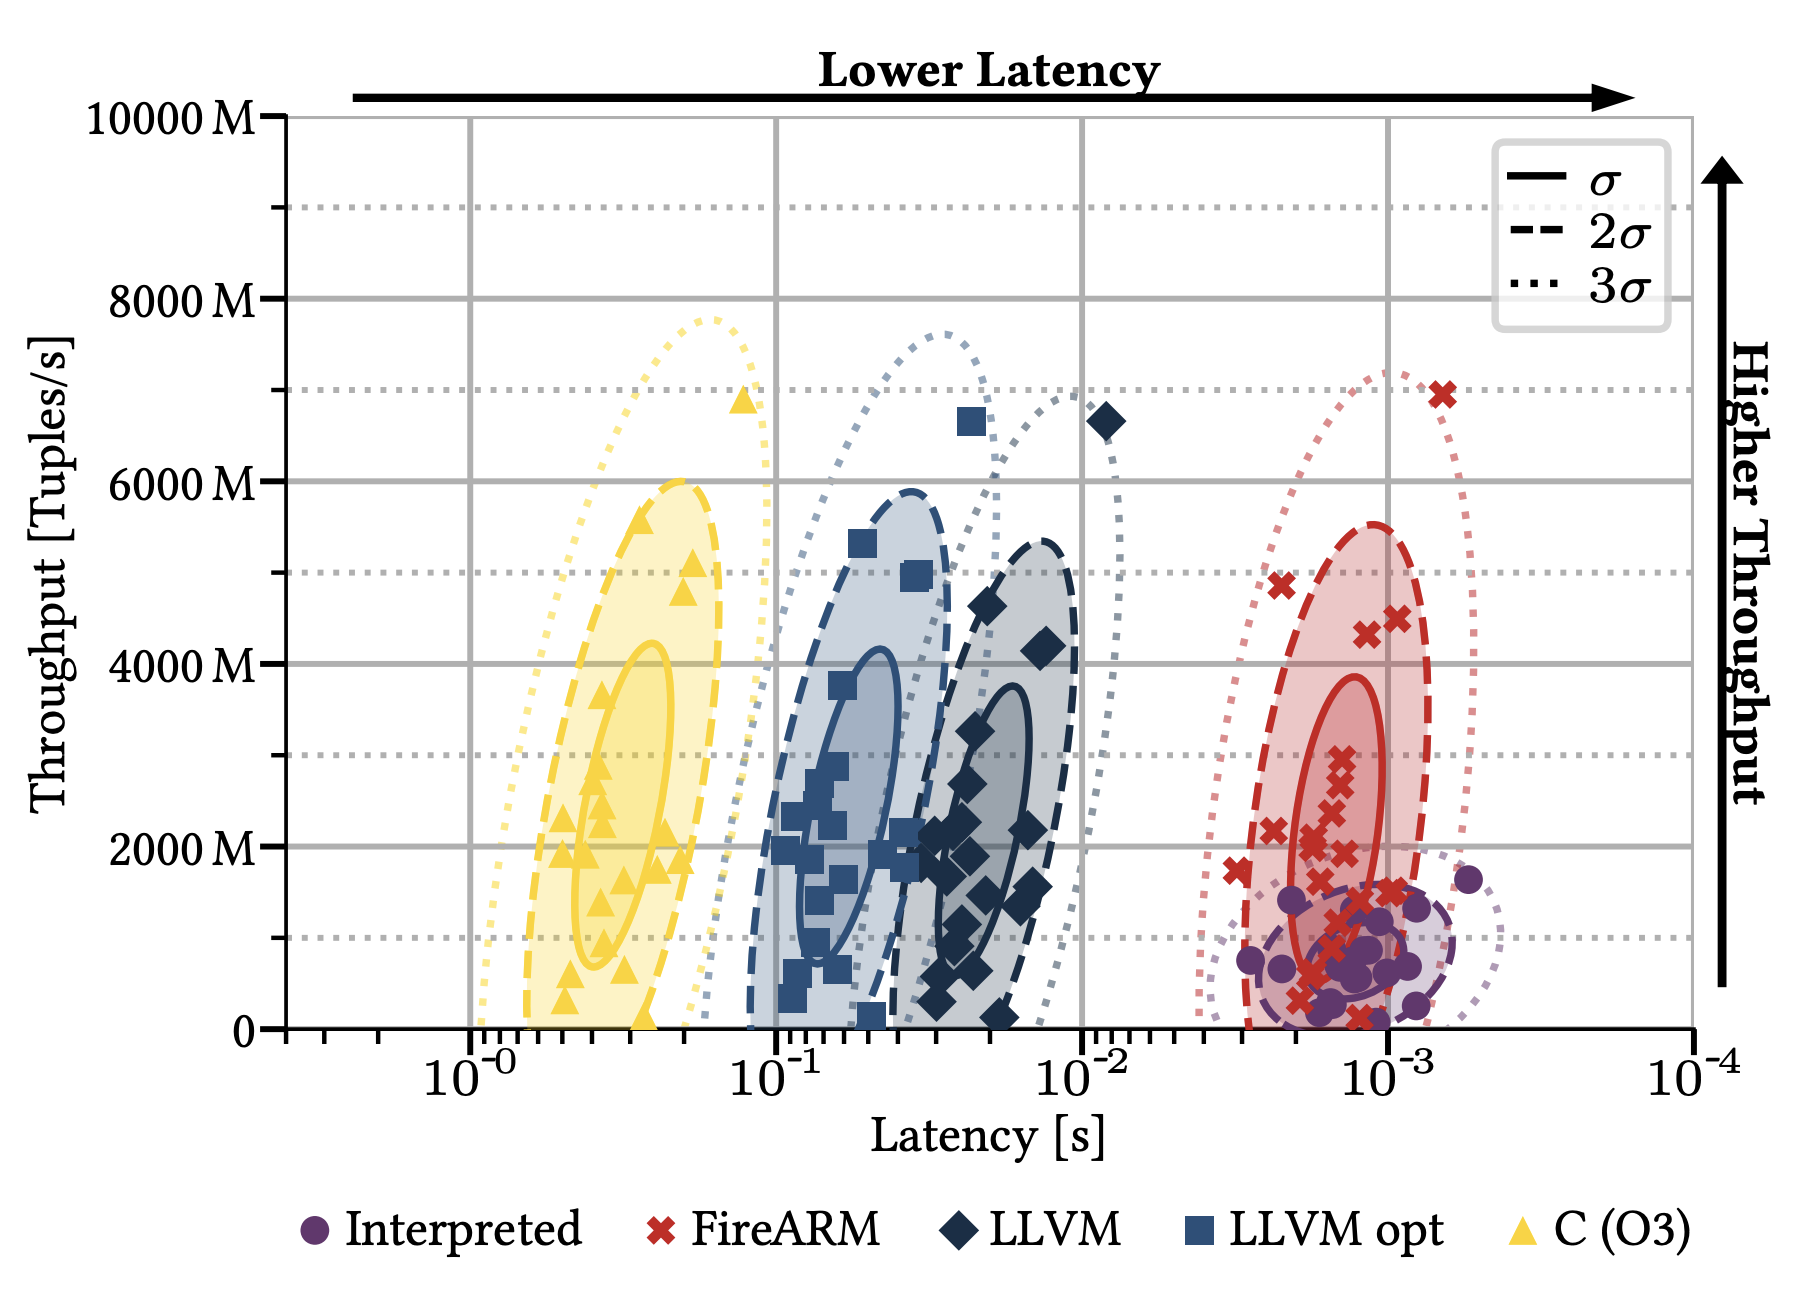
\includegraphics[width=0.8\linewidth]{figures/risc-metrcis-visualization.png}
  \caption{Visualisation example of compile-time and throughput of different query-compilation strategies running the TPC-H benchmark \cite{Bringin-Compiling-Databases-to-RISC}.}
  \label{fig:risc-metrics}
\end{figure}

\noindent

The visualisation presents a scatter plot that groups query results into clusters, with each cluster representing a database instance by a distinct color. The Y-axis displays the throughput in tuples per second, while the X-axis shows the latency in seconds, which is a descending value from left to right. Additionally, arrowed labels point to the preferred values: higher values on the Y-axis and lower on the X-axis. Thus, top-right-corner values represent optimal performance, allowing viewers to quickly identify well-performing database instances as well as the performance differences between instances.\\
In this illustration, the system highlighted in red is notable for its low latency and high throughput. Conversely, the system marked in yellow has the poorest latency performance. The instance in purple also stands out, boasting the lowest latency, but it lags behind in terms of throughput.

In the context of performance metrics, the Benchy Viewer should be capable of visualizing the key differences between instances in an intuitive and effective way. 

Besides grouping the query results into clusters, with each cluster representing a database instance, it would also be beneficial to have the flexibility to choose a specific metric for this categorization. For instance, if a database developer is primarily concerned with the metrics of execution time and throughput, they should have the option to shape the data visualisation based on these metrics.

Up next, we'll explore the dataset that is consumed by the Benchy Viewer to offer all the data and performance metrics within the analytical visualisations. We'll detail the data structure and how the data is prepared to get in this shape.

\section{Used Datasets and Data Structure}
\subsection{Description of the Utilized Performance Data}
\subsection{Structure of the CSV File with Performance Measurements}
\subsection{Data Preparation}



% !TeX root = ../main.tex
% Add the above to each chapter to make compiling the PDF easier in some editors.

\chapter{Implementation}\label{chapter:implementation}
\textcolor{red}{TODO: Chapter Introduction}


\section{Concept: Features and Interaction Capabilities of the App}
In this section, we explore the expected features and capabilities crucial for our objectives and the necessary interaction capabilities from an end user's perspective.\\
We start with the visualization capabilities of the benchmark data, where the goal is to easily identify performance bottlenecks. This involves pinpointing interesting queries with distinct performances for subsequent in-depth analysis.\\
For deeper analyzing and achieving a profound understanding of diverse performance results within queries, the application should support a focus on individual queries. Users should be able to view the performance of a single query from various perspectives, providing a comprehensive image. Comparative analysis across queries from different database systems or even the same database but with different configurations is also essential.\\ 
Then, we examine the requirements for a suitable dashboard that contains the main part of the performance visualizations. Multiple views are necessary to construct a complete understanding of the current point of interest. The optimal structure of these views can vary depending on the point of interest. The flexibility of a drag-and-drop solution for structuring views allows users to tailor the overview according to their specific interests.\\
Finally, we examine the capability of the system to facilitate collaboration and knowledge sharing. The application should enable the saving and sharing of potential findings. This involves saving the interface configuration of the analysis for sharing with other users. Recipients should be able to upload the received configuration, gaining access to the same data and visualization structure for collaborative exploration.


\subsection{Visualizing Benchmark Data}
Visualizing Benchmark Data includes multiple aspects. It involves the import of the actual data, where a proper way of importing the data should be provided. We also cover the utilized plots and charts for the data visualization. In addition to visualization, we offer a comprehensive table view of the data.


\subsubsection{Charts and Plots}

We aim to offer a dashboard containing multiple data views. To prevent UI clutter, a universal legend of database system instances is suitable, eliminating the necessity to display a legend in every chart. In the legend depicted in Figure~\ref{fig:legend} all database systems included in the benchmark data are presented as colored toggles, allowing users to activate or deactivate their appearance in the visualization. We dive deeper into the interactive legend in \ref{sec:query-analytics}.

\begin{figure}[h]
    \centering
    
\includegraphics[width=1\linewidth]{figures/legend.png}
    \caption{Gobal Legend showing all participating Database Systems.}
    \label{fig:legend}
  \end{figure}



When initiating the analytical process with the Benchy Viewer after importing the benchmark data, it may be beneficial to start with a general and straightforward overview of the benchmark data for quickly gaining an understanding of the general performance standings of the database systems.\\
Within the Benchy Viewer, this overview is effectively conveyed through the relative performance visualization, as depicted in Figure~\ref{fig:relative-performance}. This chart displays, on the Y-Axis, the relative performance of each system in percentage compared to the best-performing system in the benchmark data. The X-Axis lists and represents every database system contained in the benchmark data.

\begin{figure}[h]
  \centering
  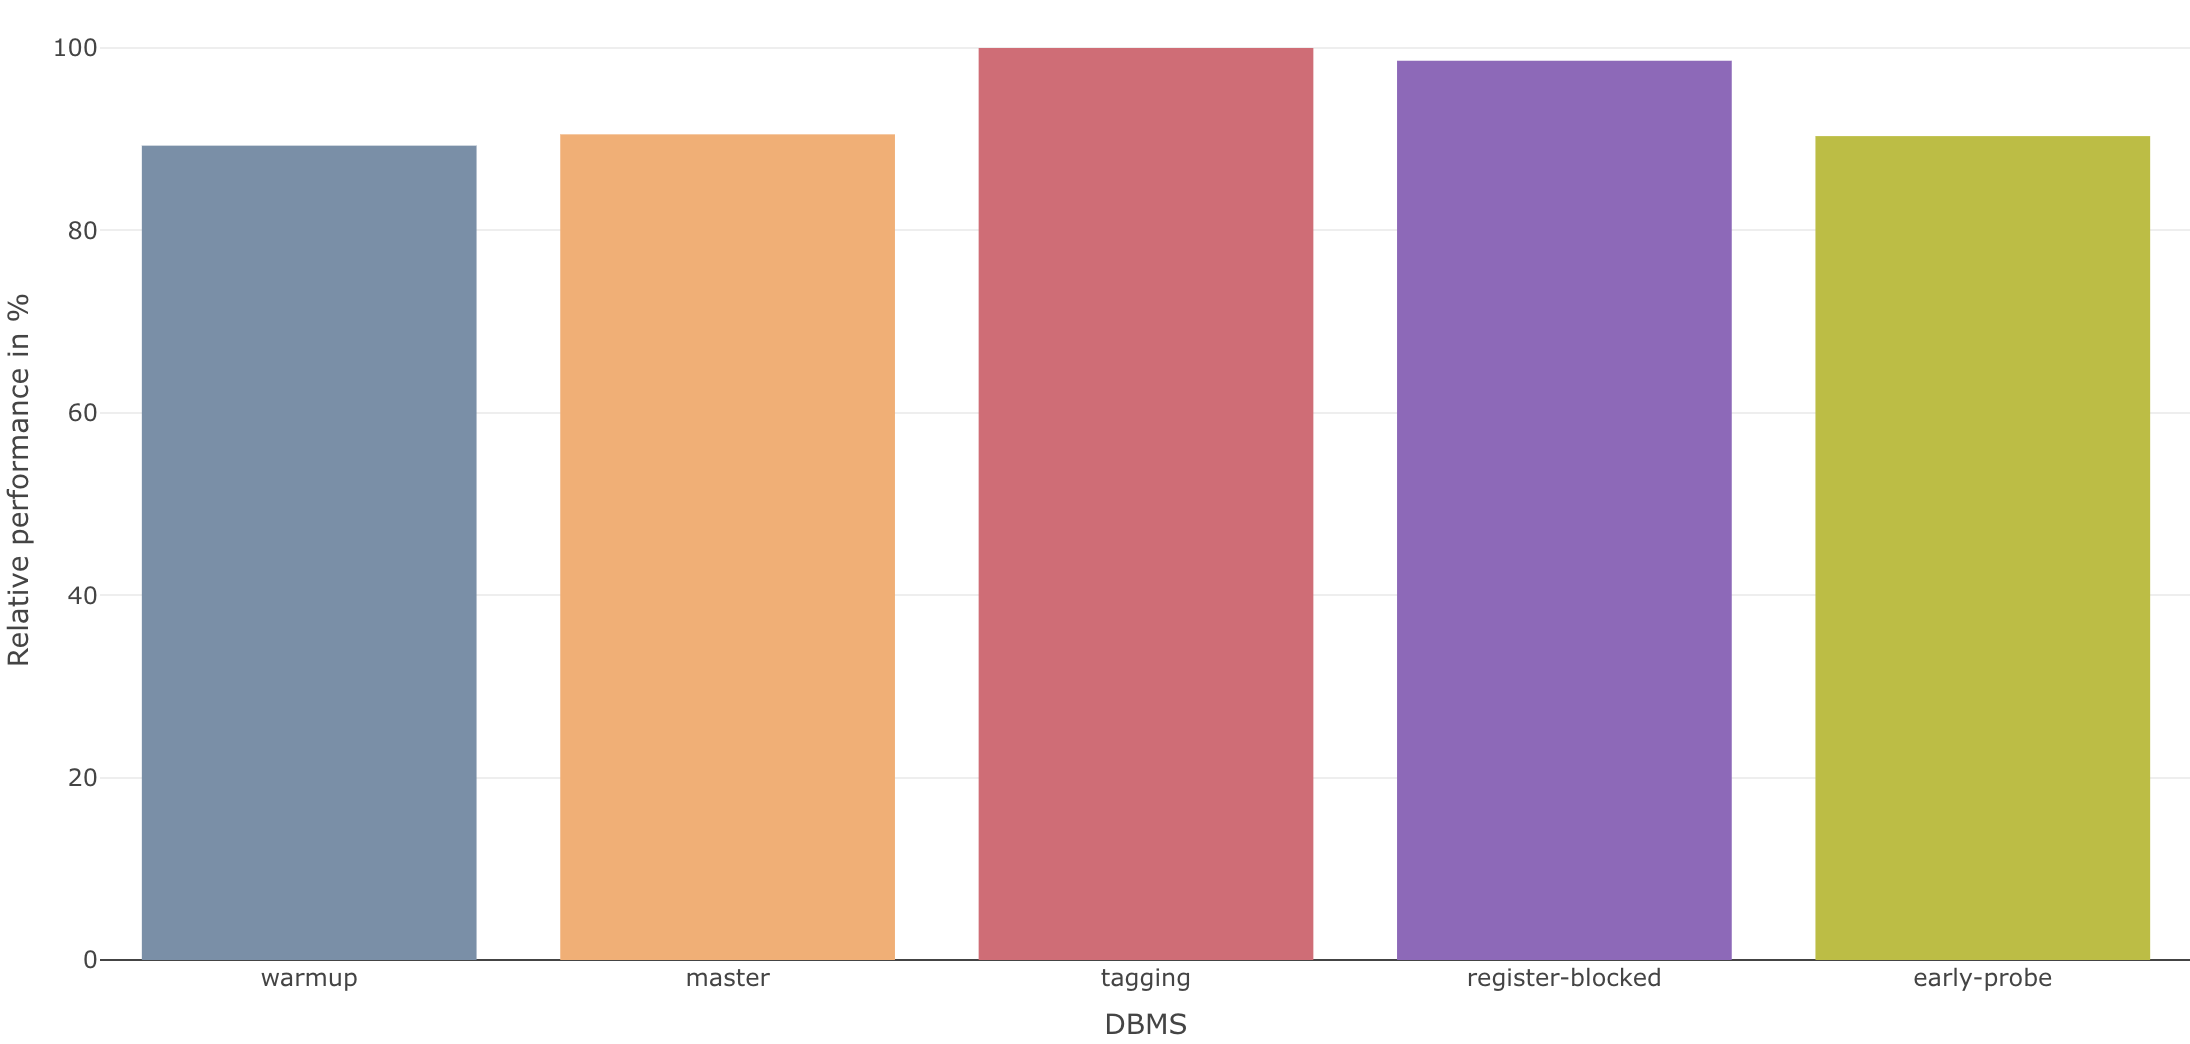
\includegraphics[width=1\linewidth]{figures/bsp-relative-performance.png}
  \caption{Bar chart visualizes the relative performance of all systems compared to the best performing system.}
  \label{fig:relative-performance}
\end{figure}

After obtaining this initial overview, users can quickly identify the system marked with the red color as the benchmark, as it processes all queries faster than all other systems. In this visualization, this system is set as the benchmark with 100\% performance, providing a clear reference point for relative comparisons.\\
This chart serves as a valuable starting point for further in-depth analyses and allows users to grasp the overall performance landscape before delving into specific metrics or queries.

In the next phase of the analysis process, we delve into two crucial aspects: compilation and execution. Compilation is the phase where source code is translated into machine code, preparing it for execution. It is a crucial step that impacts the overall performance of the system. On the other hand, execution is the phase where the compiled code is run on the system. This step involves the actual processing of the instructions and the generation of results. The time spent in the execution phase is a key factor in determining the system's efficiency in handling tasks.

To understand how much time each database system allocates to these processes, the Benchy Viewer offers a stacked bar chart, illustrated in Figure~\ref{fig:execution-compilation}. Here, one section of the bar signifies the time spent in the compilation step, while the other represents the time spent in the execution step.

\begin{figure}[h]
  \centering
  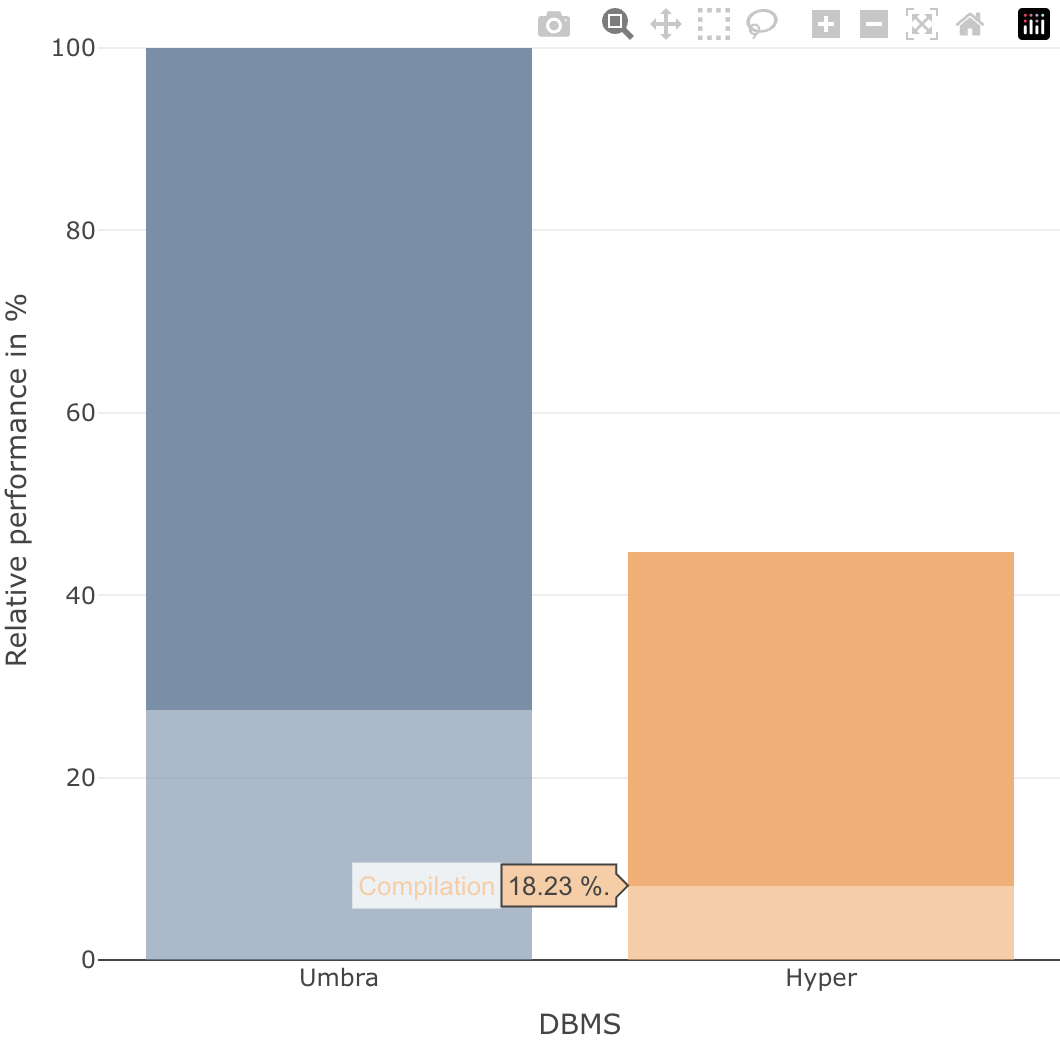
\includegraphics[width=0.5\linewidth]{figures/bsp-compilation-execution.png}
  \caption{Stacked Bar Chart illustrating the Distribution of Time between Compilation and Execution steps: The compilation step is depicted in a transparent accent color, while the execution step is represented in the full color intensity.}
  \label{fig:execution-compilation}
\end{figure}

Using solely the ratio of the two different steps, without taking into account the overall performance, would present an incomplete picture of the balance between the two process steps compared to the better-performing systems. Therefore, this chart complements the relative performance visualization discussed earlier. By incorporating information about the overall performance, it aims to offer a comprehensive understanding while illustrating the equilibrium between compilation and execution for each system.

In this example, a comparison is made between two database systems, with the Y-Axis indicating the relative performance and the X-Axis listing different database systems. Umbra stands out as the best-performing system, with its bar reaching the 100\% level. In contrast, Hyper attains 45\% of Umbra's performance. When hovering over one of the process steps, the chart displays the percentage of the total time spent by the system in that specific step. For instance, Hyper allocated 18.23\% of the entire process to the compilation step, while Umbra spent 27\% on this phase.

Hence, the stacked bar chart in the Benchy Viewer offers a consolidated view of how each database system allocates time between compilation and execution steps. Its integration of the relative performance metric ensures a balanced understanding of system efficiency, preventing oversights from focusing solely on step ratios. With clear visual distinctions and the ability to compare multiple systems, this chart enhances analytical insights into performance disparities and offering an aerial view of compilation and execution.

The preceding visualization solution \textcolor{red}{Referenz auf PDF} shows essential benchmark visualizations, offering both a comprehensive overview of all queries and a detailed examination of each individual query.

It commences with a comparative analysis of each query using a bar chart. Similar to Figure~\ref{fig:bar-chart}, this chart displays queries from various database systems on the X-Axis, with the total time presented on the Y-Axis. 

\begin{figure}[h]
    \centering
    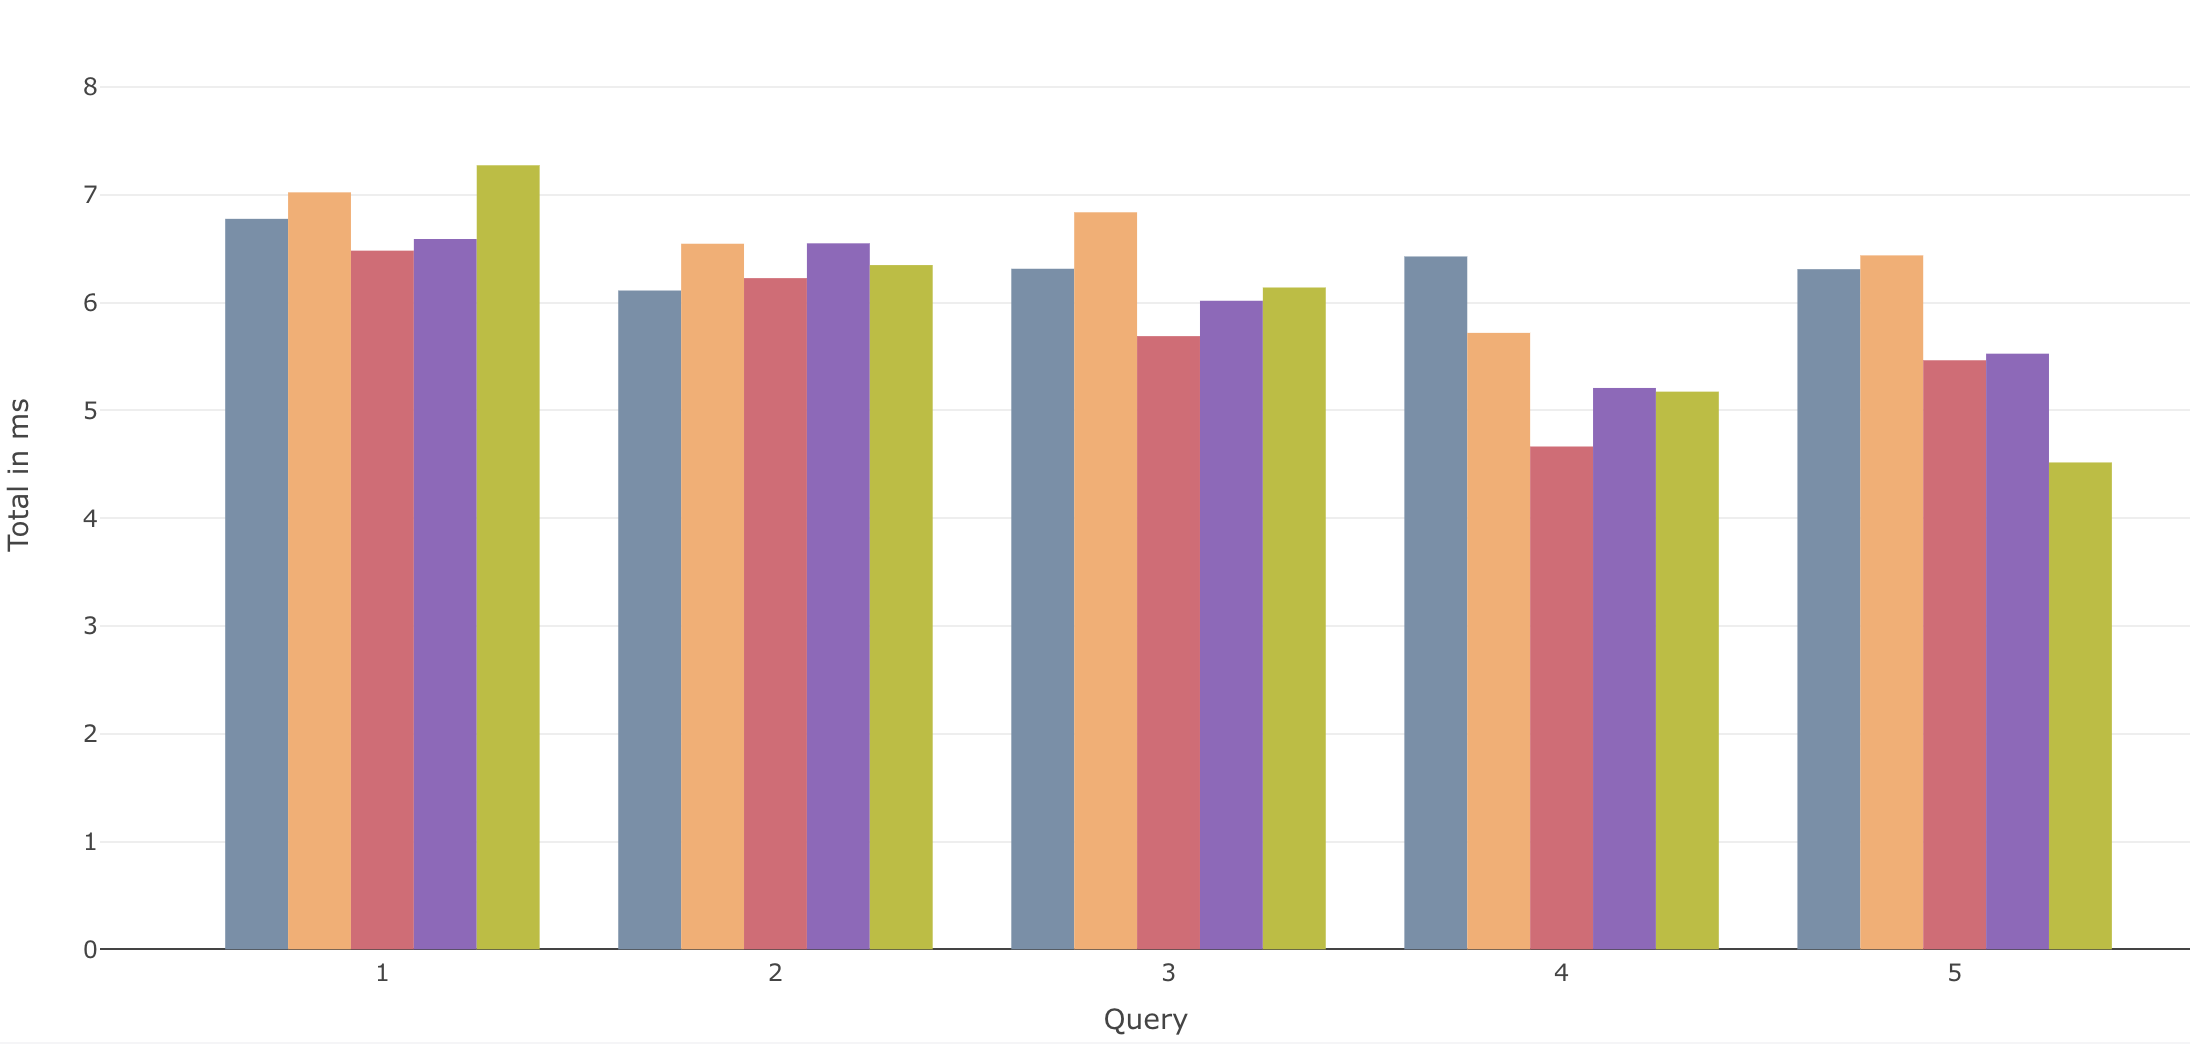
\includegraphics[width=1\linewidth]{figures/bsp-bar.png}
    \caption{Bar chart visualizes the totals time in ms of different queries.}
    \label{fig:bar-chart}
  \end{figure}

Bar plots stand out as a versatile visualization method, particularly when tasked with presenting the performance metrics of multiple queries. Their inherent clarity, with the length of each bar directly corresponding to a specific performance metric such as compilation time or execution time, makes them well-suited for diverse scenarios.\\
With each query distinctly represented by a separate bar, variations in performance become immediately apparent.\\
This quality proves especially valuable for our objective of identifying outliers, as these exceptional values are easily noticeable.

To facilitate a quick and clear overview of all queries, violin charts are employed. These charts not only provide an initial glimpse of the overall system performance but also offer distribution insights, including the shape and density of the data. They can also be combined with boxplots to get a concise summary of the distribution of the results, displaying key statistics such as the median and quartiles.

\begin{figure}[h]
    \centering
    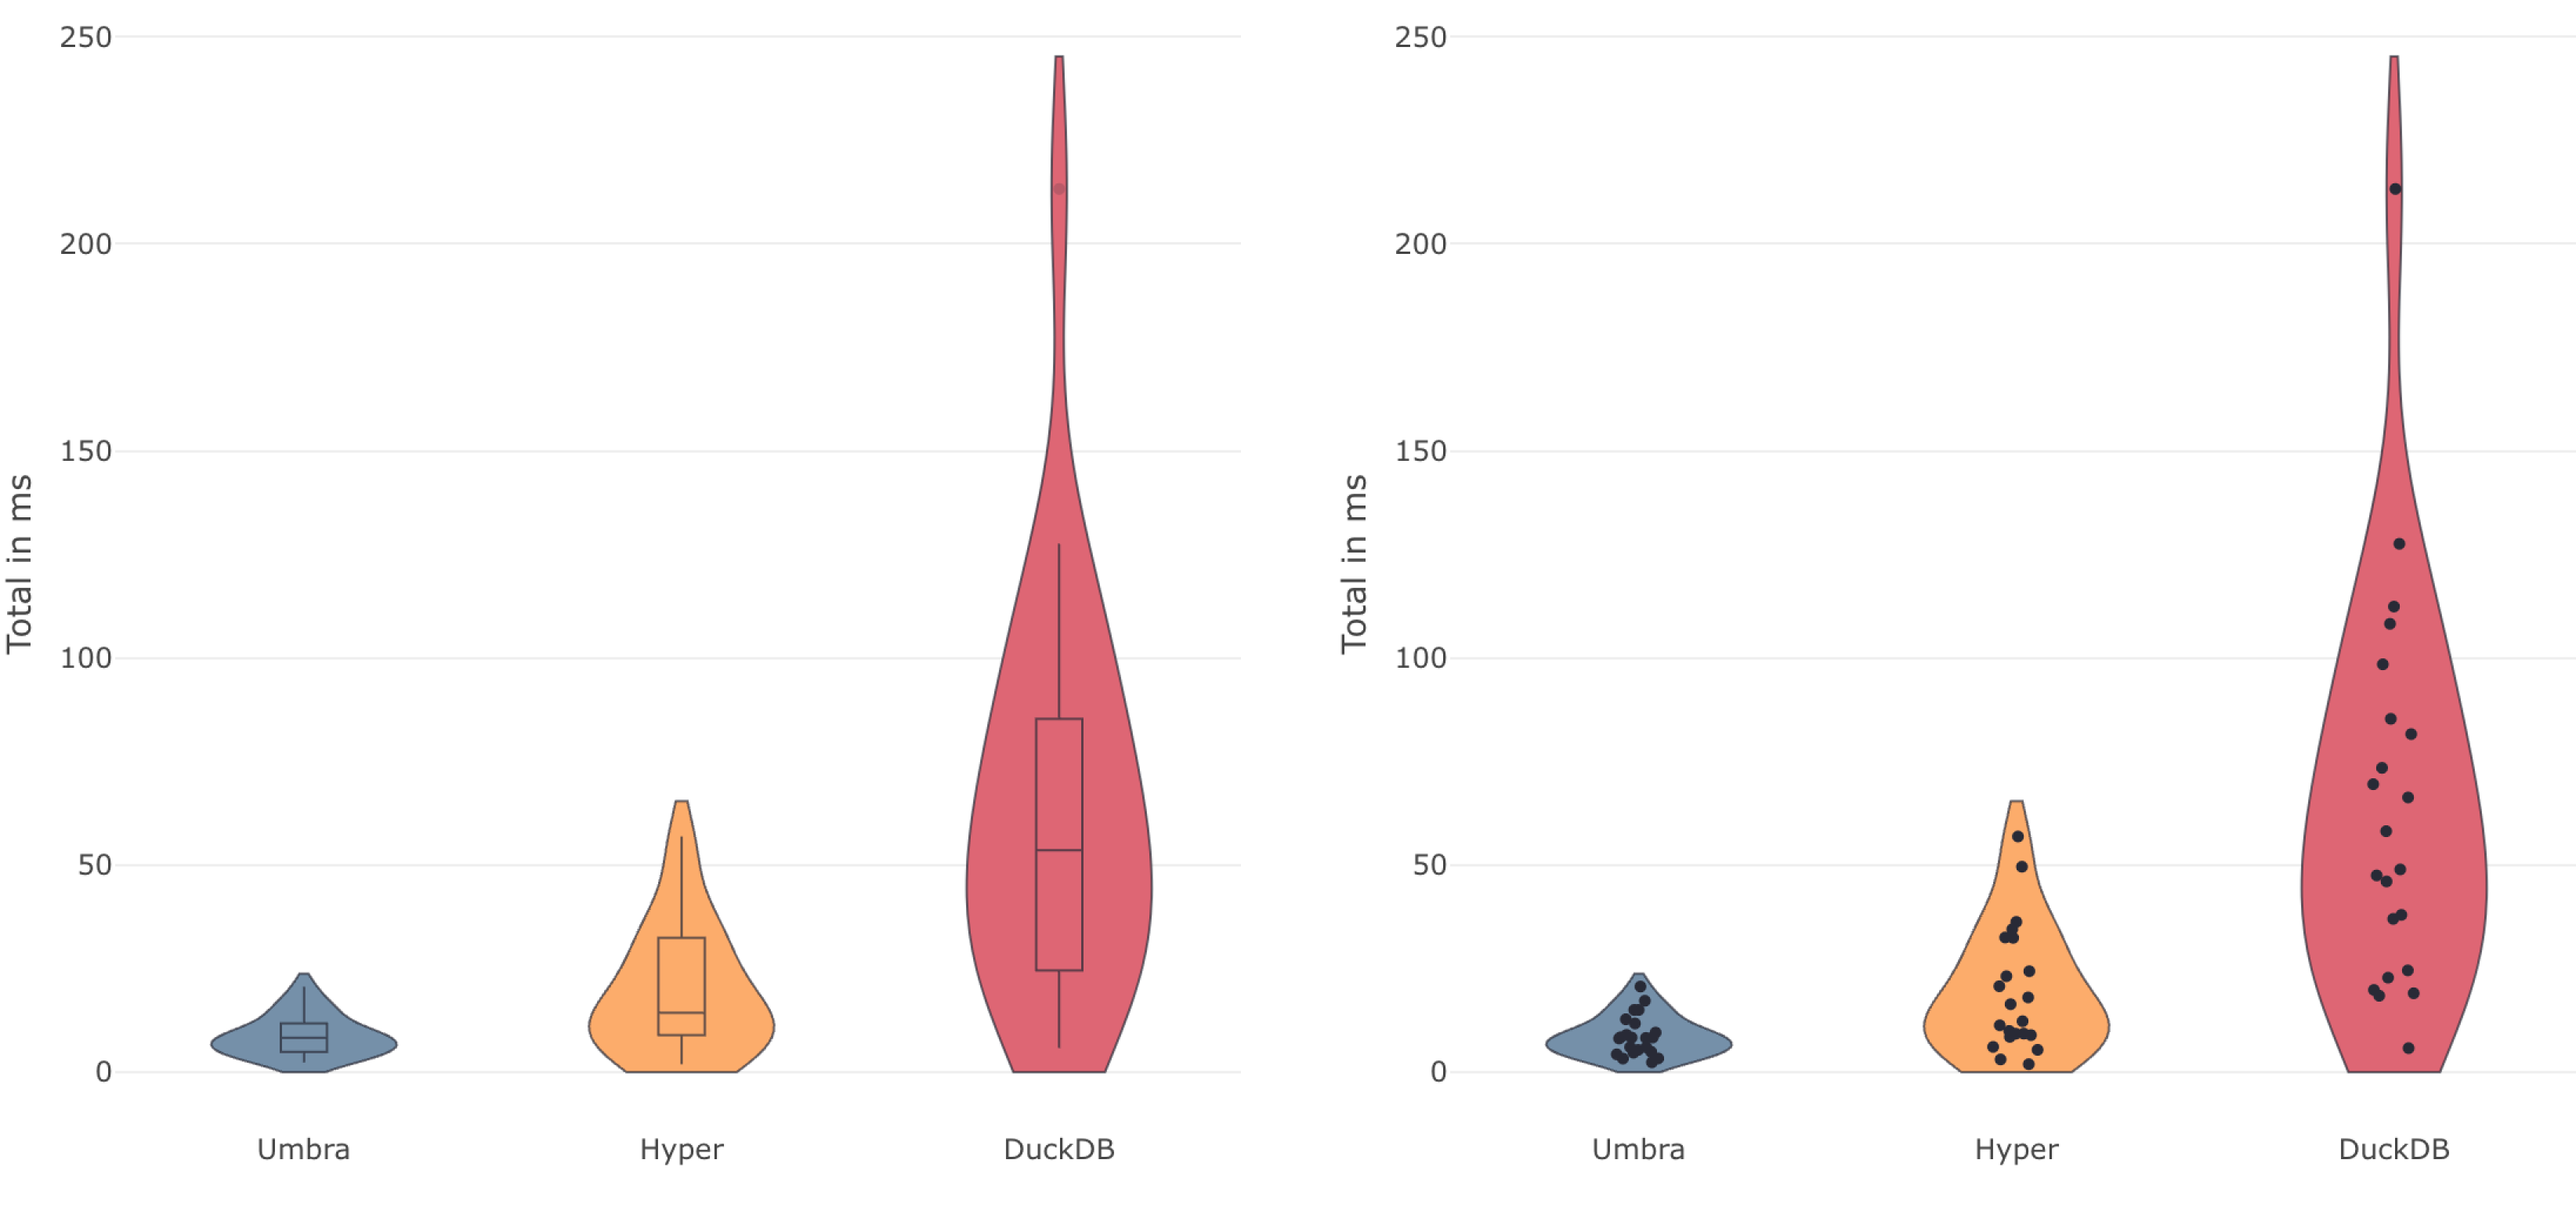
\includegraphics[width=1\linewidth]{figures/bsp-violin-boxplot-points.png}
    \caption{Violin charts visualize the totals time in ms of different queries. The left variant contains a boxplot and the right variant contains all data points.}
    \label{fig:violin-chart}
  \end{figure}

Within the Benchy Viewer violin plots that contain data points, as shown in Figure~\ref{fig:violin-chart} on the right side, additionally allow you to hover over a data point. This action highlights the corresponding query in the violins of the other database systems. We will explore this hover feature further in \ref{sec:hover-feature}.


Conducting benchmark performance analysis often necessitates a comparative approach between a chosen system and other competing systems. The Benchy Viewer facilitates this by enabling the selection of a baseline system from one of the database systems included in the benchmark data, as shown in Figure~\ref{fig:select-baseline-system}.

\begin{figure}[h]
  \centering
  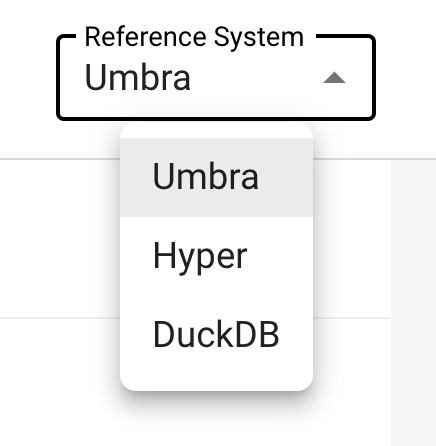
\includegraphics[width=0.3\linewidth]{figures/select-baseline-system.png}
  \caption{A drop-down menu that allows to select a baseline system.}
  \label{fig:select-baseline-system}
\end{figure}


This functionality proves useful for assessing how the performance of the chosen baseline system compares to others, aiding in the identification of strengths, weaknesses, and potential optimization areas. It forms a foundational step in the detailed analysis provided by the Benchy Viewer. Several visualizations in the application utilize the baseline system, including the table view and scatter plot for inspecting the slowdown and speedup metric, and the bar chart showcasing the performance delta for each query from the perspective of the baseline system. All these visualizations depend on a baseline system, making this functionality crucial for a comprehensive performance analysis.

In the context of providing a clear and comparative understanding of how different systems perform relative to a chosen baseline, the metrics maximum slowdown and maximum speedup become crucial. They offer a comprehensive view of the range of performance variations. Maximum slowdown indicates the worst-case scenario of reduced performance, while maximum speedup highlights the most significant improvement achieved.

\textbf{Slowdown} indicates how much faster a specific system is compared to the baseline system. It is calculated as the ratio of the time taken by the system under consideration to the time taken by the baseline system. A slowdown value greater than 1 implies that the system is slower than the baseline. For example, a slowdown of 1.5 means the system is 1.5 times slower than the baseline.\\
Identifying slowdowns is crucial for pinpointing areas of inefficiency or performance bottlenecks in a system. It helps in understanding where improvements are needed.

\textbf{Speedup}, on the other hand, quantifies how much slower a specific system is compared to the baseline system. It is calculated similarly to slowdown but in the reverse manner. A speedup value greater than 1 implies that the system is faster than the baseline. For example, a speedup of 2 means the system is twice as fast as the baseline.\\
Knowing the speedup is essential to highlight improvements. It indicates the effectiveness of optimizations or enhancements made to the system compared to the baseline.

The Benchy Viewer employs tables to showcase the maximum slowdown and maximum speedup, visualized in Figure~\ref{fig:slowdown-speedup-chart}, where the maximum slowdown is displayed on the left side and the maximum speedup on the right side using Umbra as the baseline system. The use of cell colors in the table serves as an effective visual indicator of performance outliers. Intensity in color corresponds to the extent of the outlier, offering a rapid understanding of the range and distribution between these extreme values. This color-coded representation aids users in identifying and assessing the significance of performance variations across different systems.

\begin{figure}[h]
  \centering
  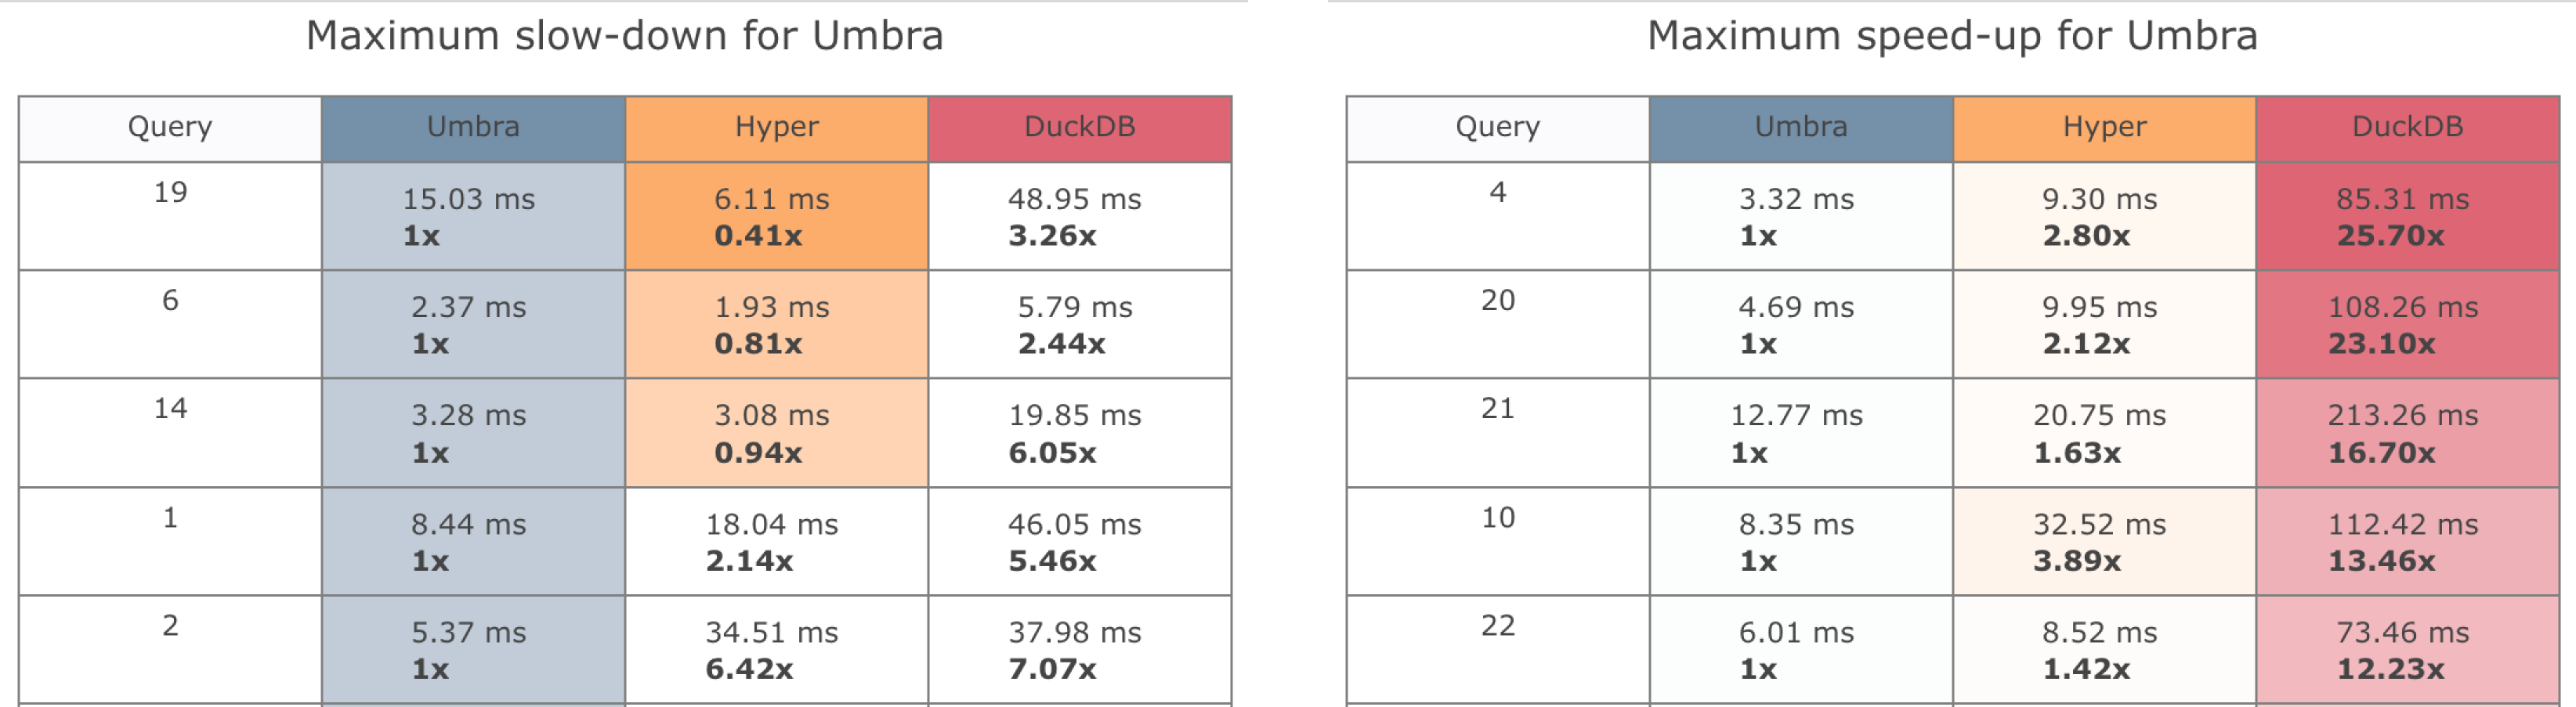
\includegraphics[width=1\linewidth]{figures/bsp-table-speedup-slowdown.png}
  \caption{Tables showcase the maximum slowdown and the maximum speedup using color intensity to indicate performance outliers.}
  \label{fig:slowdown-speedup-chart}
\end{figure}

The tables are organized based on the resulting ratio. In the maximum slowdown tables, the arrangement is ascending, placing the slowest queries of the baseline system compared to the faster alternative system at the top.\\
Conversely, in maximum speedup tables, the sorting is descending, presenting the fastest queries of the baseline system compared to the alternative system at the forefront. This sorting strategy provides a logical structure to quickly identify and compare performance differences in either scenario.

The scatter plot is another effective choice for visualizing speedup and slowdown. These plots are particularly beneficial for trend analysis, offering a detailed view of each query individually. Users can identify trends, clusters, or outliers in the data, providing insights that might be less apparent in a table.

In the Benchy Viewer a baseline is displayed, as illustrated in Figure~\ref{fig:scatter} positioned at Y = 1 and colored in blue. This positioning allows users to observe the relative performance of each query compared to the baseline system.

\begin{figure}[h]
  \centering
  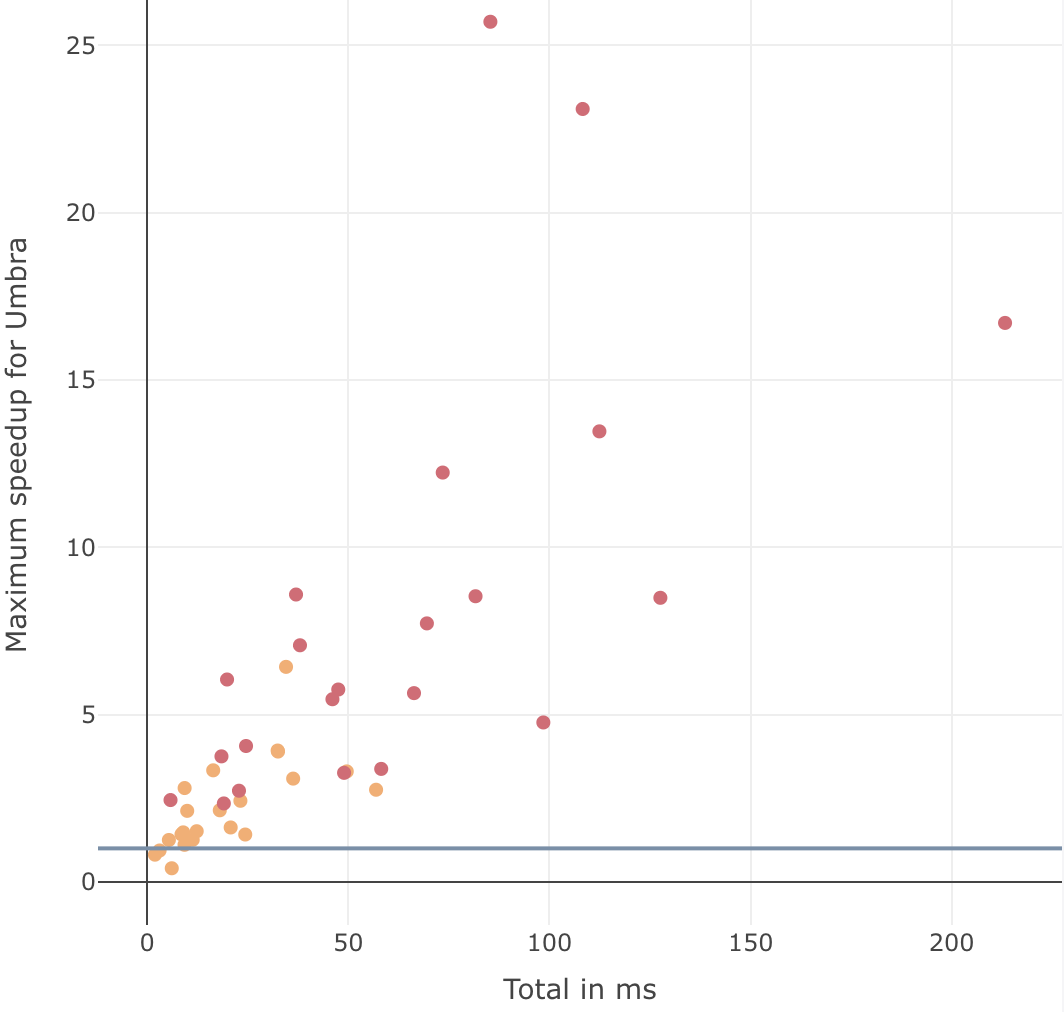
\includegraphics[width=0.7\linewidth]{figures/bsp-scatter.png}
  \caption{Scatter Plot visualizes the speedup.}
  \label{fig:scatter}
\end{figure}

In this example, the scatter plot represents the maximum speedup for the selected baseline system on the Y-axis, while the total time in milliseconds is represented on the X-axis. This visualizes the relationship between the total time taken by each query and its corresponding speedup compared to the baseline system.\\
Hovering above these query data points reveals the ratio of the corresponding speedup and the query identifier. We will explore the hover feature further in \ref{sec:hover-feature}.\\
Queries from the competing system are marked in orange, and most of them are slower, with three queries below the baseline, indicating that these particular queries are faster.\\
This observation prompts further investigation into the queries below the baseline, offering an opportunity to identify potential performance bottlenecks from the perspective of the baseline system. This nuanced understanding, facilitated by the visual representation of the scatter plot, guides users in pinpointing specific queries that deviate from the expected performance trend, aiding in targeted optimizations and analysis.

In the Benchy Viewer, another visualization occurs, highlighting the performance disparities between a chosen baseline system and its competitors. It takes the form of a bar chart that illustrates the performance gap for each query, providing a perspective of the baseline system compared to the best-performing query of other competing systems.

The performance delta chart in the Benchy Viewer not only displays the performance gap for each query from the perspective of the baseline system but also indicates the best competing system for each query by using corresponding system colors, as depicted in Figure~\ref{fig:performance-gap}. The Y-axis shows the performance gap percentage of the competing queries, while the X-axis represents the identifying query number. Hovering over bars reveals the exact performance delta.

\begin{figure}[h]
  \centering
  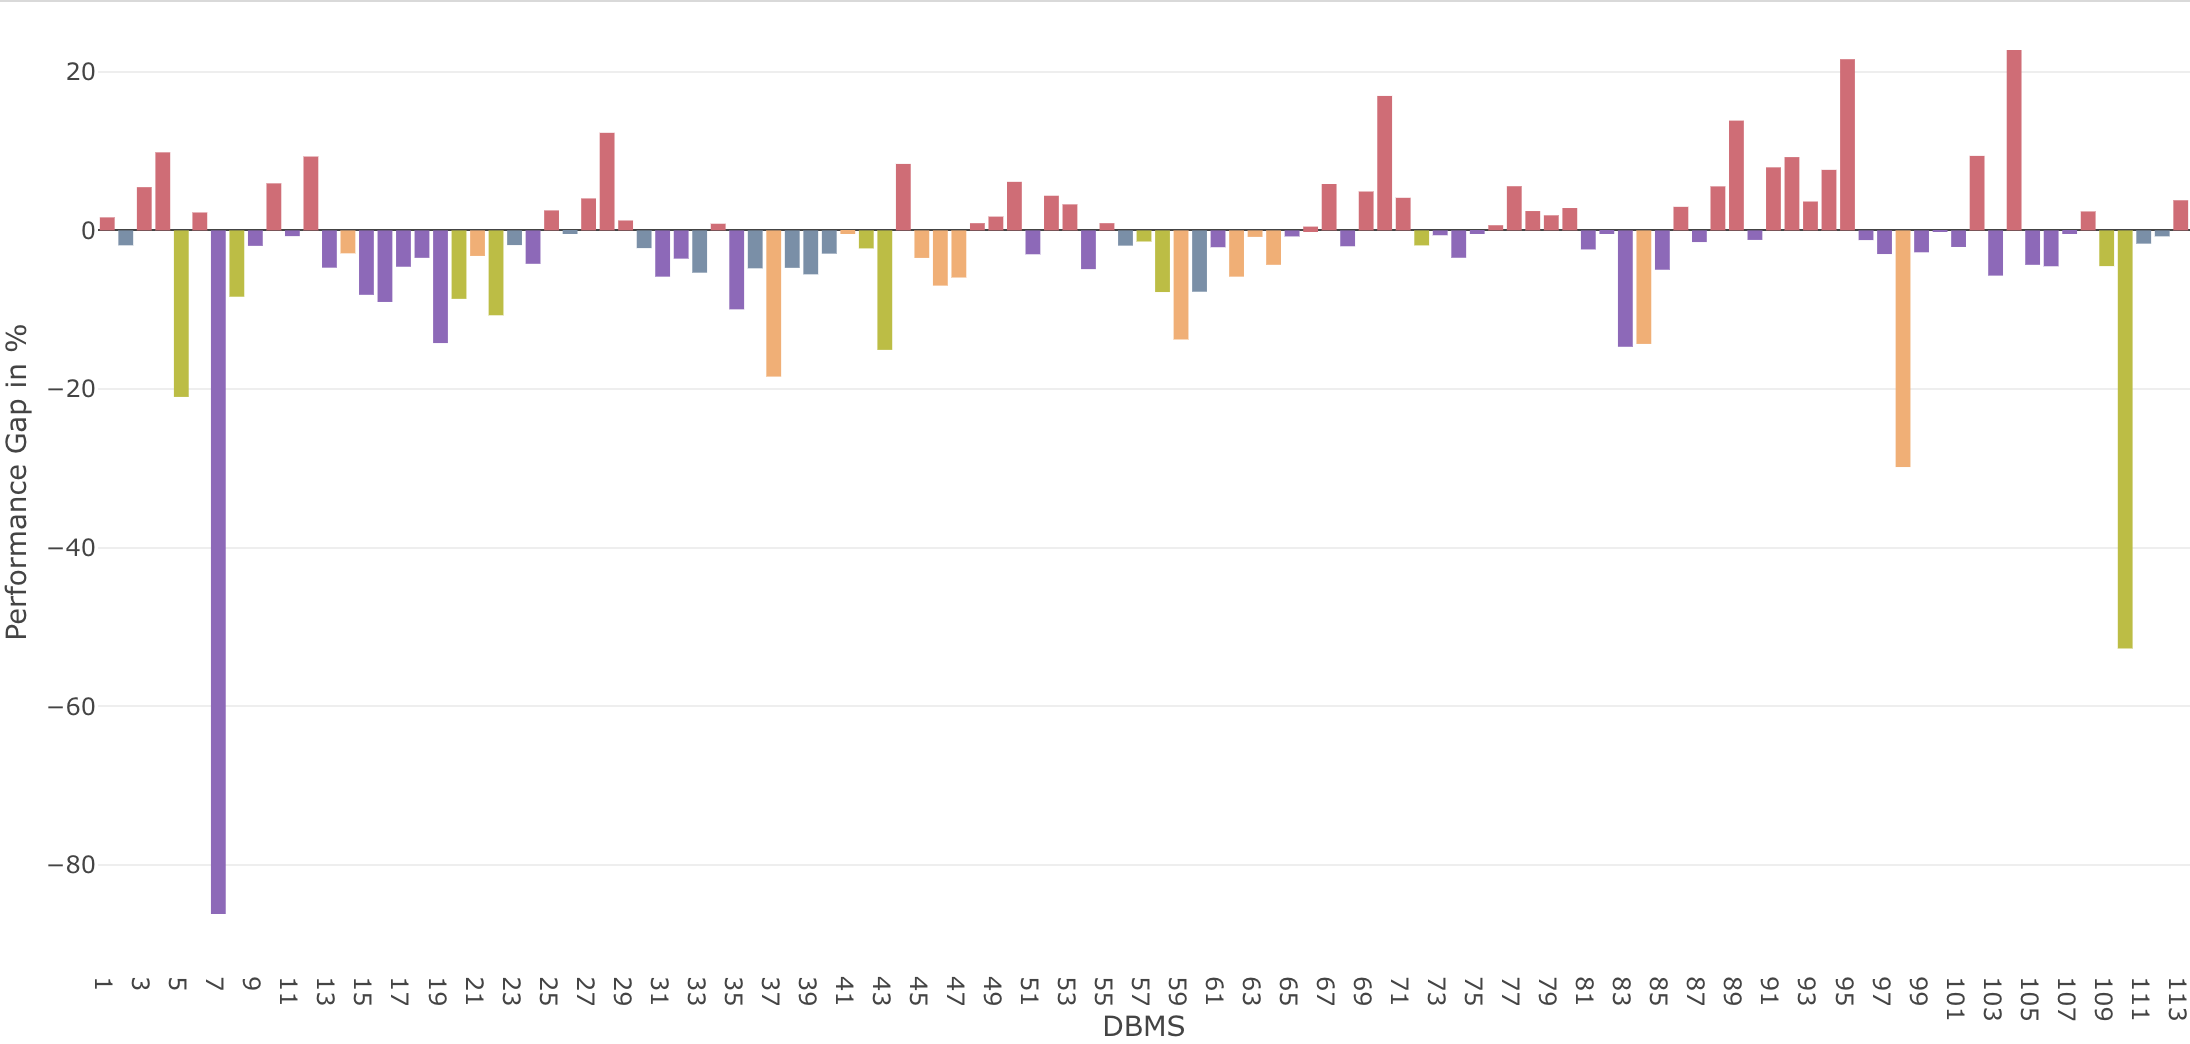
\includegraphics[width=1\linewidth]{figures/bsp-query-gaps.png}
  \caption{Bar chart visualizes the performance gap for every query of the baseline system compared to best corresponding query of the competing systems.}
  \label{fig:performance-gap}
\end{figure}

In this example, the red-marked database system is selected as the baseline system. Queries with faster performance by the baseline system are displayed above the baseline, indicating a positive performance delta. In contrast, queries with stronger performance by competing systems are shown below the baseline, indicating a negative performance delta for the baseline system. Additionally, the bar of each query is marked with the color of the corresponding best-performing database system.\\
The performance gap for the majority of cases in this example stays within a range between -20\% and 20\%. However, some outliers are notably significant. For instance, the seventh query has a performance gap of -86\%. A deeper analysis of this query may be sensible to potentially identify performance bottlenecks from the perspective of the baseline system.

This query performance gap visualization is instrumental in quickly discerning how each query of the baseline system stacks up against the top-performing queries of other systems. The chart's simplicity ensures easy comprehension, enabling users to promptly assess the relative performance of different queries.




\subsubsection{Hover Feature}\label{sec:hover-feature}

\begin{figure}[h]
  \centering
  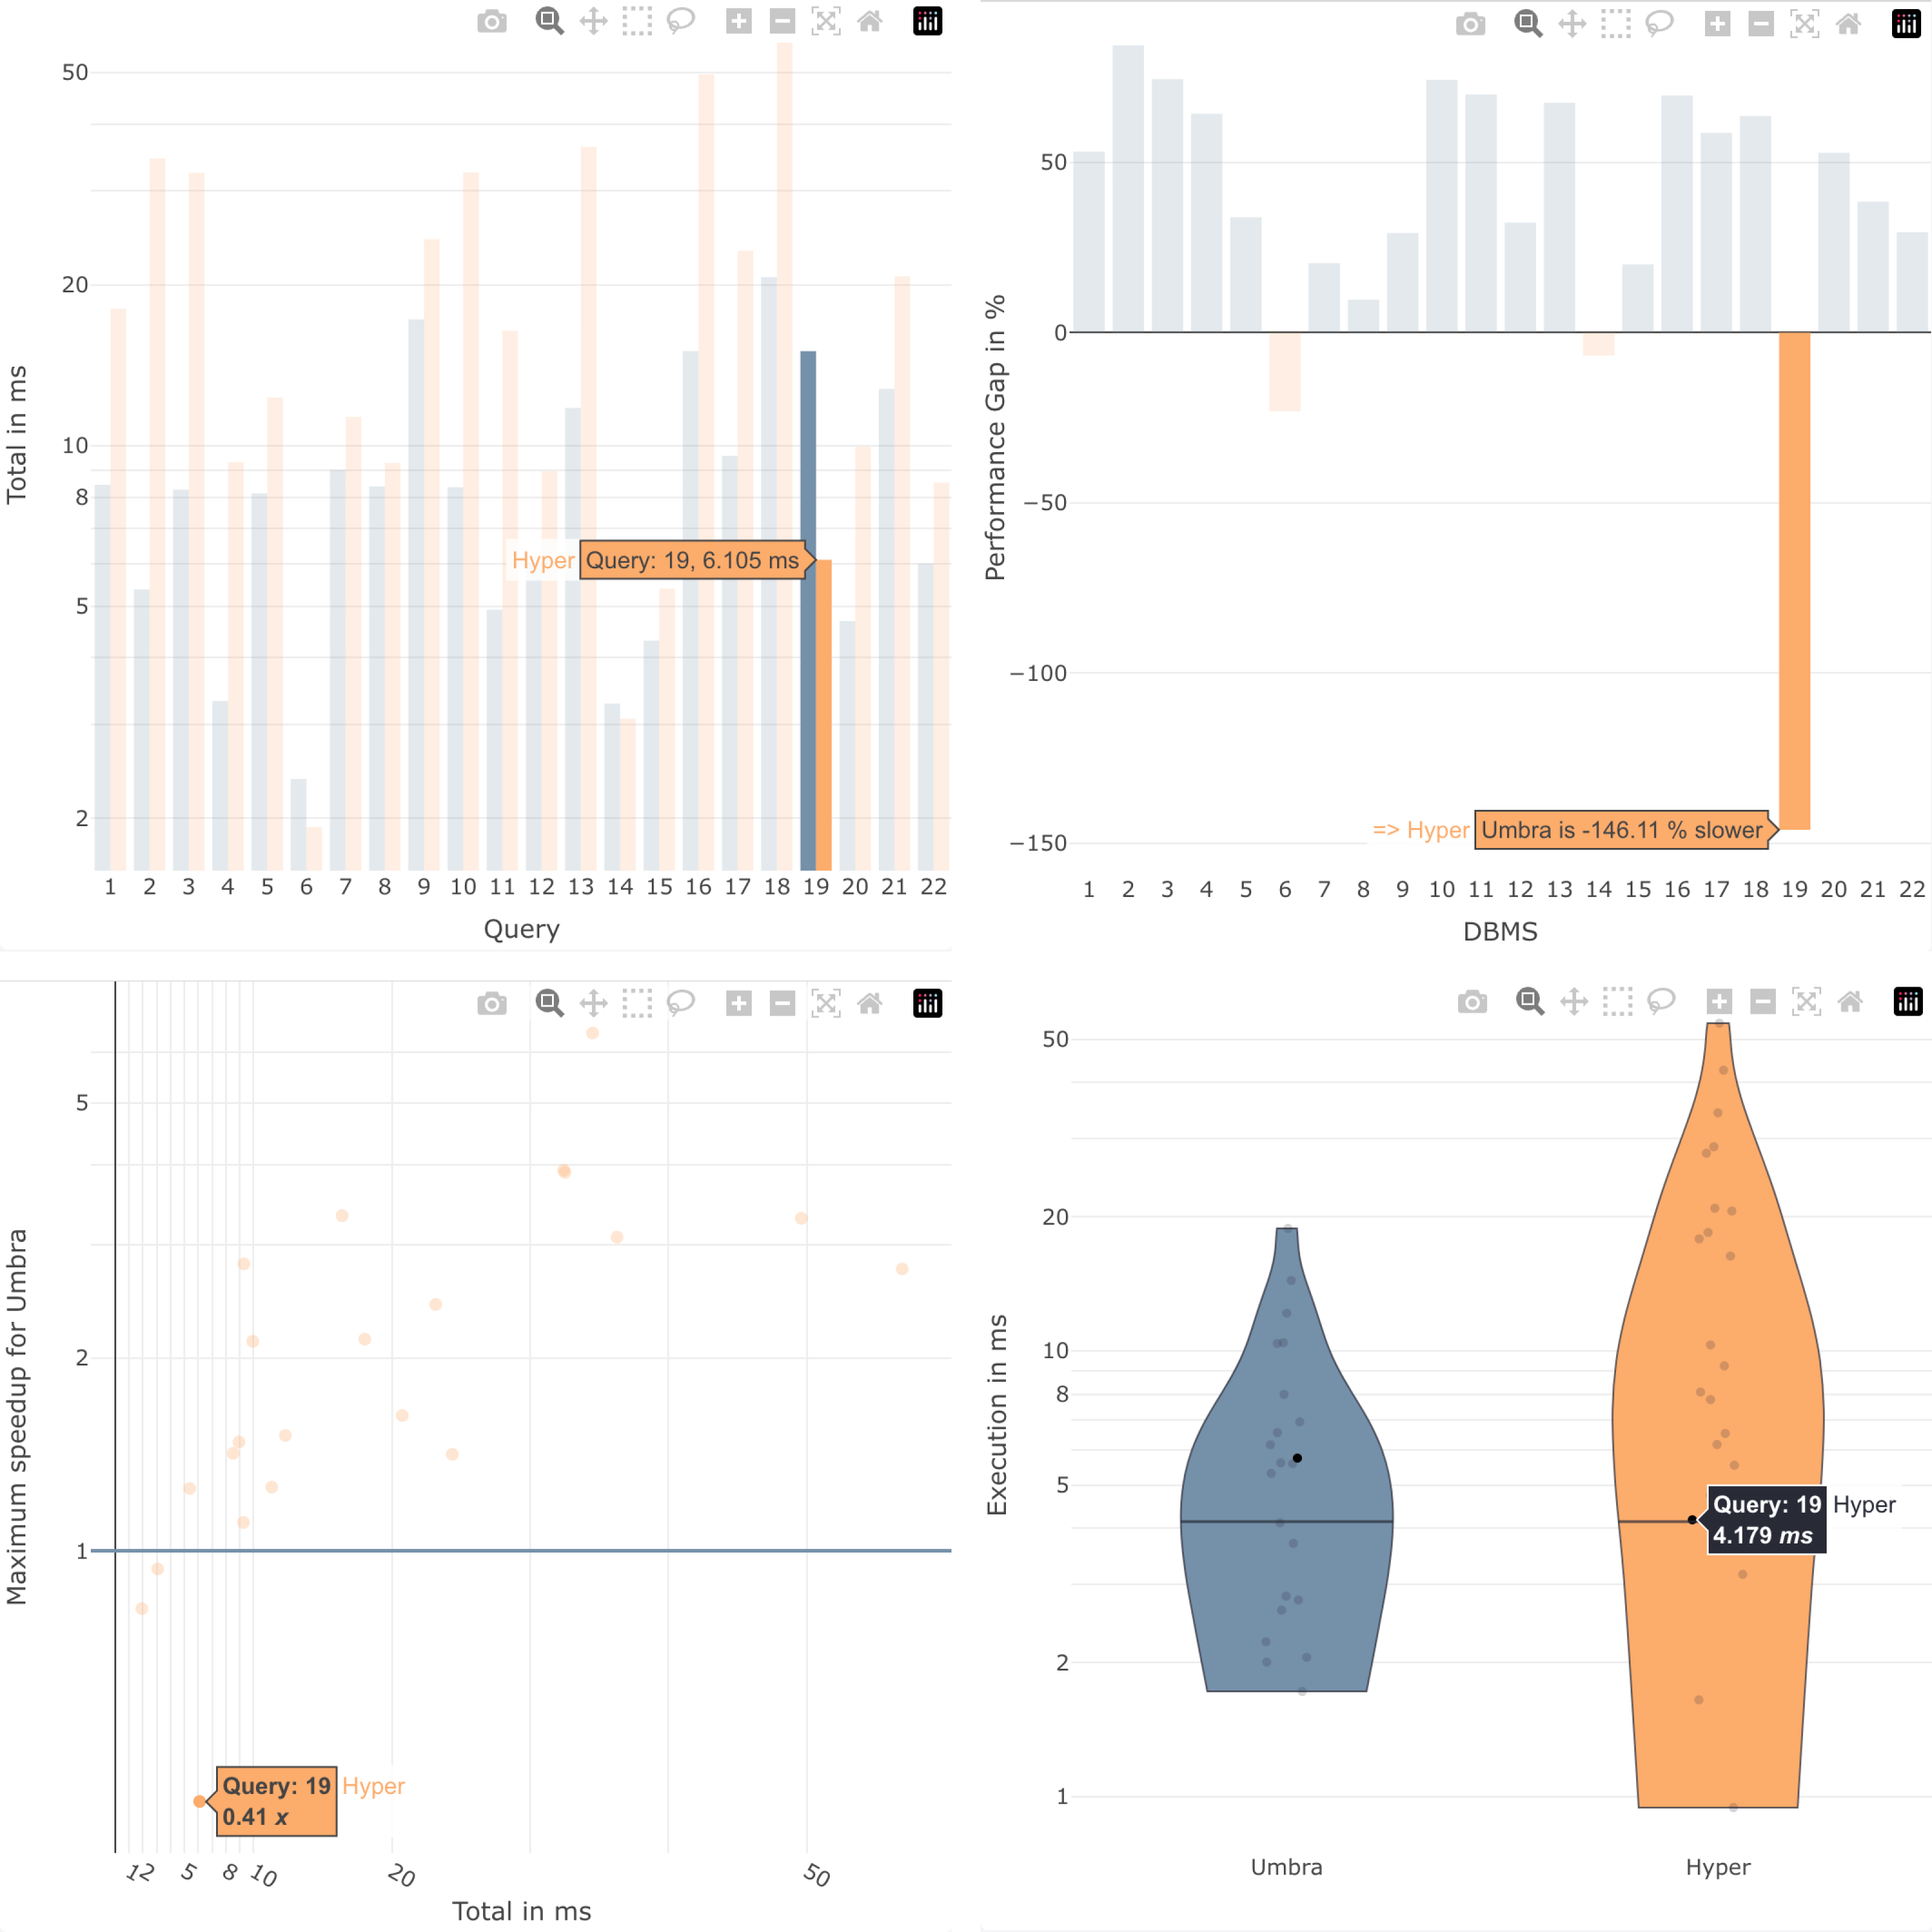
\includegraphics[width=0.6\linewidth]{figures/hover-group.png}
  \caption{Hovering over a query automatically highlights in a global context the same query in all visualizations which are showcasing single queries. These visualizations include violin plots, scatter plots, and bar charts when one bar represents a single query.}
  \label{fig:hover-group}
\end{figure}

Hovering over data points in a chart is an indispensable feature, commonly employed to extract more detailed information about a specific data point. In the context of analyzing query performances and identifying noteworthy queries within visualizations, the ability to scrutinize a particular query from multiple perspectives becomes crucial.


 In the Benchy Viewer, we've elevated this feature, which is illustrated in Figure~\ref{fig:hover-group}, to a global hover capability within the application.\\
 This means that when a user hovers over a specific query, not only is that query highlighted within the current chart, but the same queries within all other visualizations are also highlighted simultaneously. This synchronization spans various visualizations, including violin plots, scatter plots, and bar charts which represent distinct queries.\\
 With this feature, the user is able to easily identify the same queries across various visualizations, offering a comprehensive understanding from diverse perspectives.



\subsubsection{Data Viewer}

In addition to visualizations, the Benchy Viewer features a data table for in-depth inspection of benchmark data. This table presents the imported user data, as exemplified in the excerpt of the data viewer in Figure~\ref{fig:data-viewer}.

\begin{figure}[h]
  \centering
  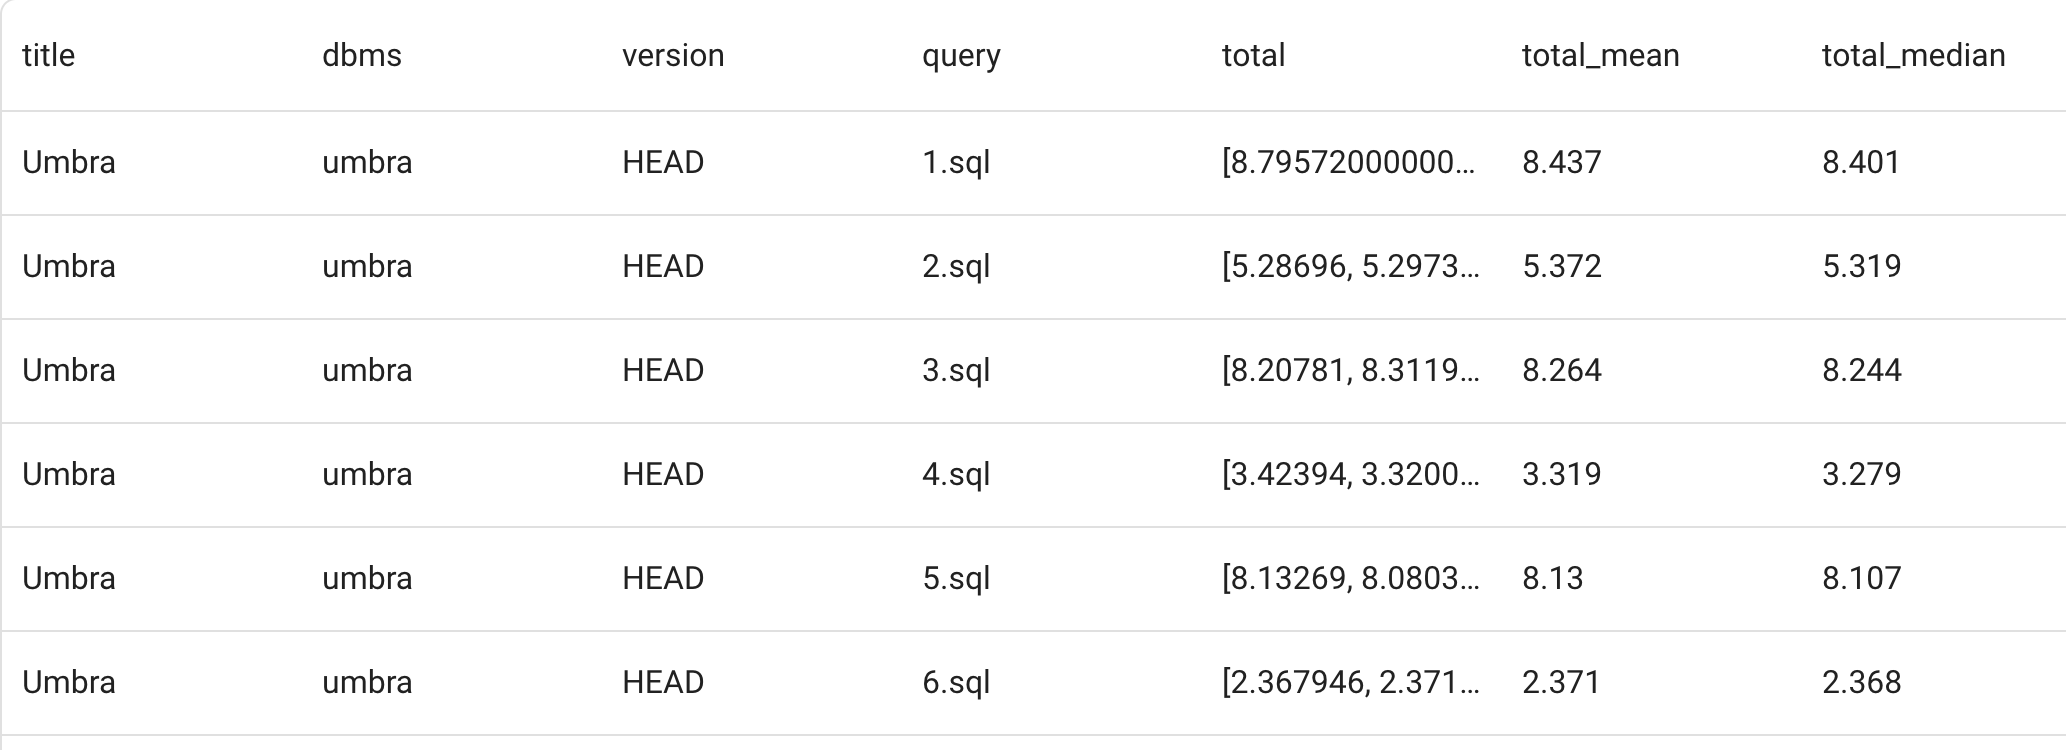
\includegraphics[width=0.9\linewidth]{figures/data-viewer.png}
  \caption{Snapshot of the Data Viewer: Organized rows and columns of benchmark data.}
  \label{fig:data-viewer}
\end{figure}

This view showcases the benchmark data, elaborately described in Section \ref{sec:input-file-structure}. The header encompasses all properties and metrics of a data row. Data rows below the header represent the data of a query, including the reference to the database system and the complete benchmark data for that query.\\
Vertical and horizontal scrolling are enabled to navigate through the extensive data rows and metrics, as the volume of information exceeds the screen's capacity.

\begin{figure}[h]
  \centering
  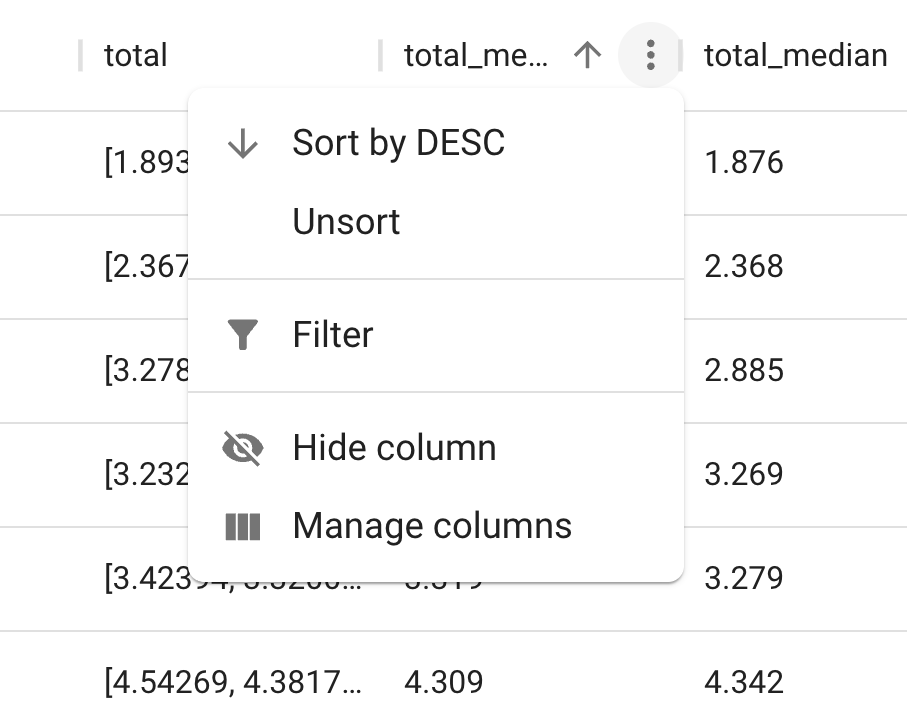
\includegraphics[width=0.4\linewidth]{figures/data-viewer-header-options.png}
  \caption{Column options drop-down offering sorting, filtering, and column visibility functionality.}
  \label{fig:data-viewer-options}
\end{figure}

The header offers various options in a drop-down menu to interact with the data sheet, as depicted in Figure~\ref{fig:data-viewer-options}.

% Sorting
The first option enables sorting the table based on a selected data column with numerical values. Users can choose between ascending or descending order, and there's an option to reset the sorting. This functionality is particularly useful when organizing specific data, for instance, sorting the table based on total time in milliseconds.

\begin{figure}[h]
  \centering
  \begin{subfigure}[b]{0.4\linewidth}
      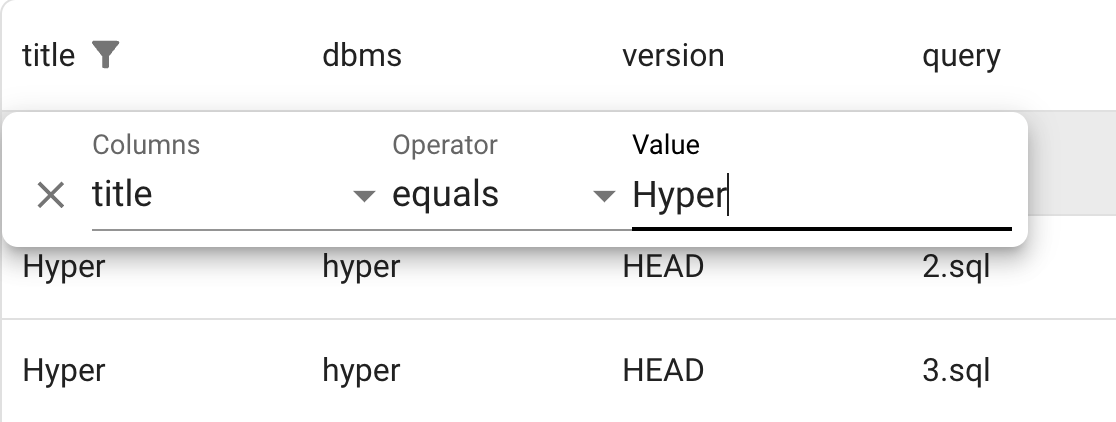
\includegraphics[width=\linewidth]{figures/data-viewer-filter.png}
      \caption{Filter Menu.}
      \label{fig:data-viewer-filter}
  \end{subfigure}
  \hspace{1cm} % Adjust the horizontal space between the figures
  \begin{subfigure}[b]{0.4\linewidth}
      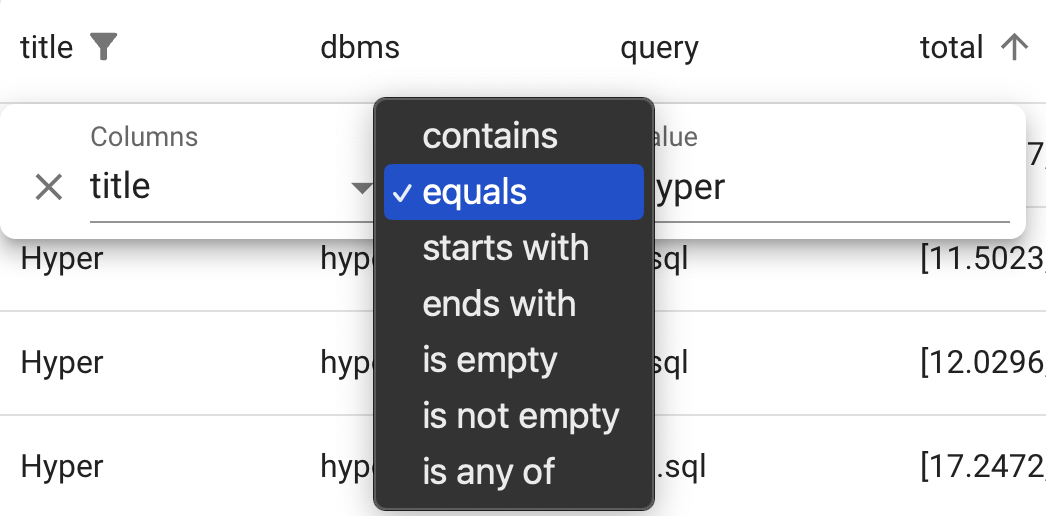
\includegraphics[width=\linewidth]{figures/data-viewer-filter-operator.png}
      \caption{The list of available operators.}
      \label{fig:data-viewer-filter-operator}
  \end{subfigure}
  \caption{Filter menu allows data sheet filtering by column, operator, and value.}
  \label{fig:combined-figures}
\end{figure}

% Filter
The filter option, as shown in Figure~\ref{fig:data-viewer-filter}, provides a tool for refining the displayed data in the table. Users can easily narrow down their focus by selecting a specific column, an operator, and a value. This allows for targeted exploration of the data, such as isolating rows related to a particular database management system, as demonstrated in Figure~\ref{fig:data-viewer-filter-operator}. This filtering capability enhances the user's ability to extract meaningful insights from the benchmark data.


% Manage Columns

\begin{figure}[h]
  \centering
  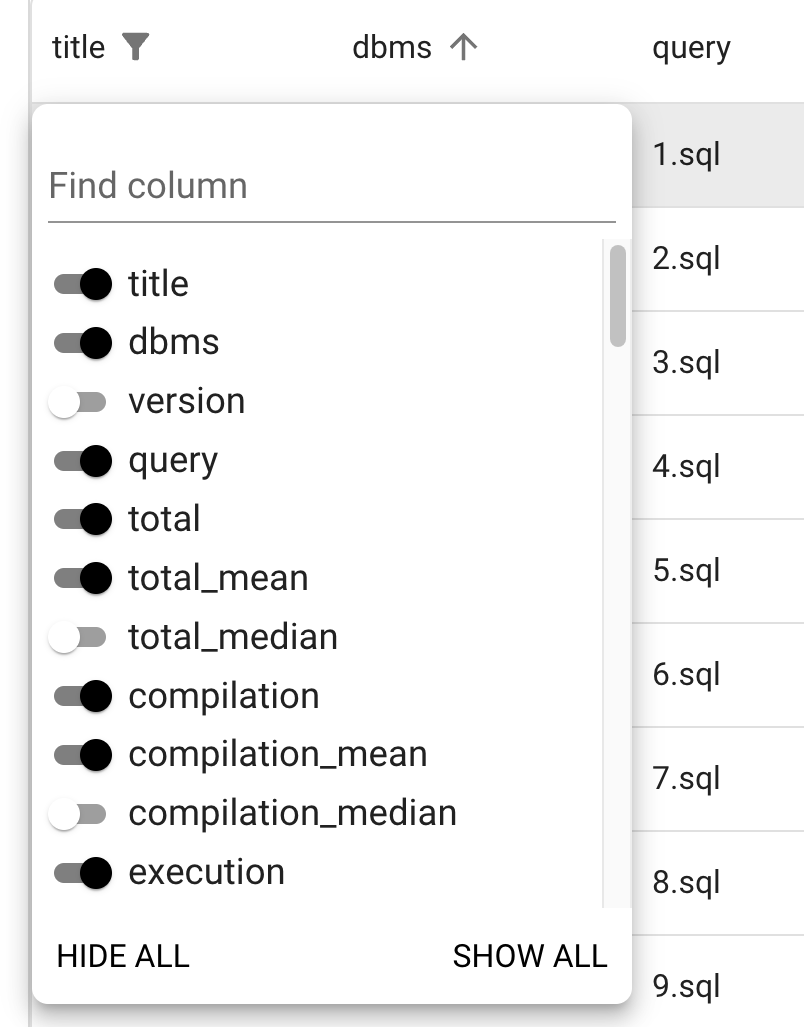
\includegraphics[width=0.35\linewidth]{figures/data-viewer-manage-columns.png}
  \caption{Column Manager: Easily control column visibility in the data sheet for a tailored view.}
  \label{fig:data-viewer-manage-columns}
\end{figure}

When dealing with extensive datasets, the Benchy Viewer ensures flexibility and ease of use by allowing users to tailor their view. Through the 'Manage columns' feature, accessed via the drop-down menu, users can not only hide columns but also gain a holistic overview of active columns. 

Figure~\ref{fig:data-viewer-manage-columns} showcases this functionality, providing users with the ability to effortlessly activate or deactivate columns, conduct quick searches, and streamline their view by hiding or showing all columns at once. This empowers users to focus on the specific data points relevant to their analysis, enhancing the efficiency of the benchmark data exploration process.




\subsection{Query Analytics: Comparative Examination and Comprehensive Benchmark Insight }\label{sec:query-analytics}

One of the primary functions of the Benchy Viewer is to conduct a comparative analysis of the performance across various database systems. The application offers a range of tools for this purpose. In addition to presenting diverse charts and plots for analyzing query data from various angles, the Benchy Viewer allows users to inspect the query plan of a selected query in a comparative manner. To initiate this process, users need to choose the particular query and the involved database systems.

\subsubsection{Preparation for In-Depth Analysis}

In the analytical process of identifying and inspecting a noteworthy query, it is beneficial to refine the information for a more precise and clear understanding.\\
The Benchy Viewer features an interactive legend that not only provides information about group colors but also offers the ability to enable or disable all query visualizations of a system throughout the entire application.

\begin{figure}[h]
  \centering
  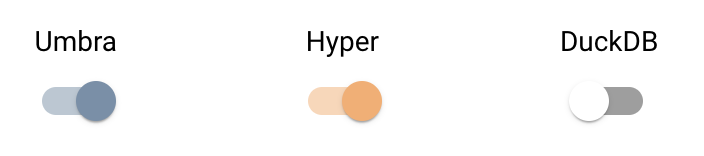
\includegraphics[width=0.4\linewidth]{figures/legend-activate-deactivate.png}
  \caption{Interactive legend with the functionality to activate or deactivate database systems.}
  \label{fig:legend-activate-deactivate}
\end{figure}

This is particularly valuable when a significant query is identified, and a comparison between two systems is of interest, while there are other less relevant systems in the data that may clutter the visualizations. In such cases, users can utilize the interactive header, illustrated in Figure~\ref{fig:legend-activate-deactivate}, to streamline their view and prioritize the visualizations based on current needs.

% Select Queries
In the course of analyzing benchmark data and identifying noteworthy queries, a deeper inspection of these queries becomes essential. The Benchy Viewer incorporates a versatile hover feature, as introduced in Section \ref{sec:hover-feature}, providing a multi-perspective view of a specific query by highlighting it across various visualizations simultaneously.

\begin{figure}[h]
  \centering
  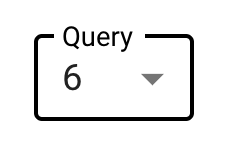
\includegraphics[width=0.15\linewidth]{figures/select-query.png}
  \caption{Drop-down for selecting a specific query for deeper inspection.}
  \label{fig:select-query}
\end{figure}

Similar to this functionality, the Benchy Viewer provides the option to directly select a specific query. This can be accomplished through various means, such as using a drop-down menu, as illustrated in Figure~\ref{fig:select-query}, or by clicking on a specific query data point within a visualization (e.g., clicking on a specific bar in a bar chart or a specific data point in a scatter plot).

Choosing a specific query results in its highlighting across all visualizations, similar to the universal hover feature demonstrated in Figure~\ref{fig:hover-group}. This enables users to concurrently emphasize two separate queries, the chosen query and a hovered one, enabling a comparative analysis from various angles.

\subsubsection{Comprehensive Query Insights}

% Query Plan
In the analysis workflow facilitated by the Benchy Viewer, once a significant query has been identified for more in-depth examination, the subsequent step involves selecting this particular query and transitioning to the Query Plan View. In this phase, users gain the ability to meticulously inspect the query plan associated with the chosen query for each database system under consideration.

The interactive legend, depicted in Figure~\ref{fig:legend-activate-deactivate}, maintains its presence in this view, allowing users to seamlessly activate or deactivate the display of query plans corresponding to specific database systems.

For clarity and comparative analysis, all activated query plans are rendered in a unified visualization. Each query plan is presented in its designated system color. This representation is exemplified in Figure~\ref{fig:query-plan-basic}, where the various query plans are harmoniously displayed for comprehensive comparative scrutiny. This visual approach not only streamlines the analysis process but also contributes to a more intuitive understanding of the comparative performance of queries across different database systems.

\begin{figure}[h]
  \centering
  \begin{subfigure}[b]{0.5\linewidth}
    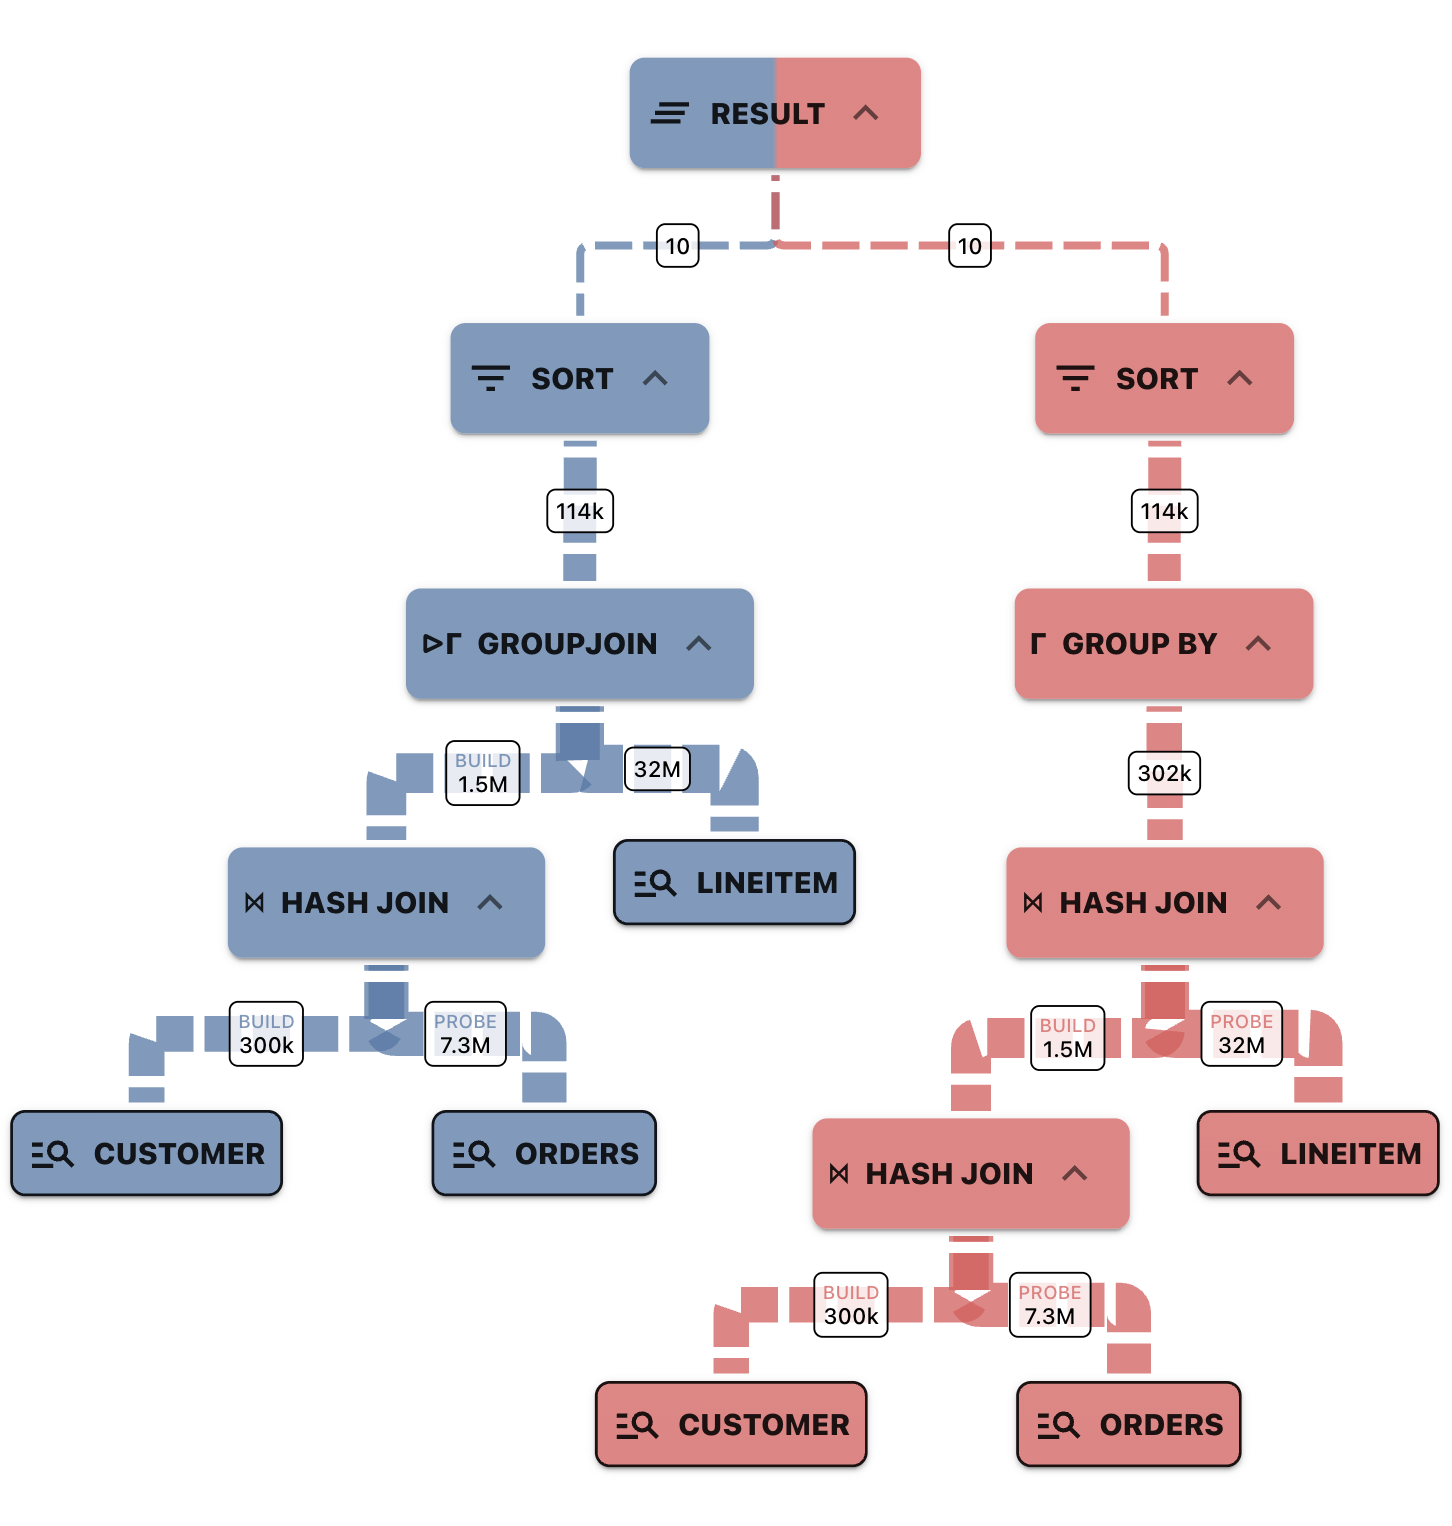
\includegraphics[width=\linewidth]{figures/query-plan-slim.png}
    \caption{Query Plan View comparing the query plan of a specific query between two database systems. The trees are displayed separately.}
      \label{fig:query-plan-basic}
  \end{subfigure}
  \hspace{1cm} % Adjust the horizontal space between the figures
  \begin{subfigure}[b]{0.4\linewidth}
      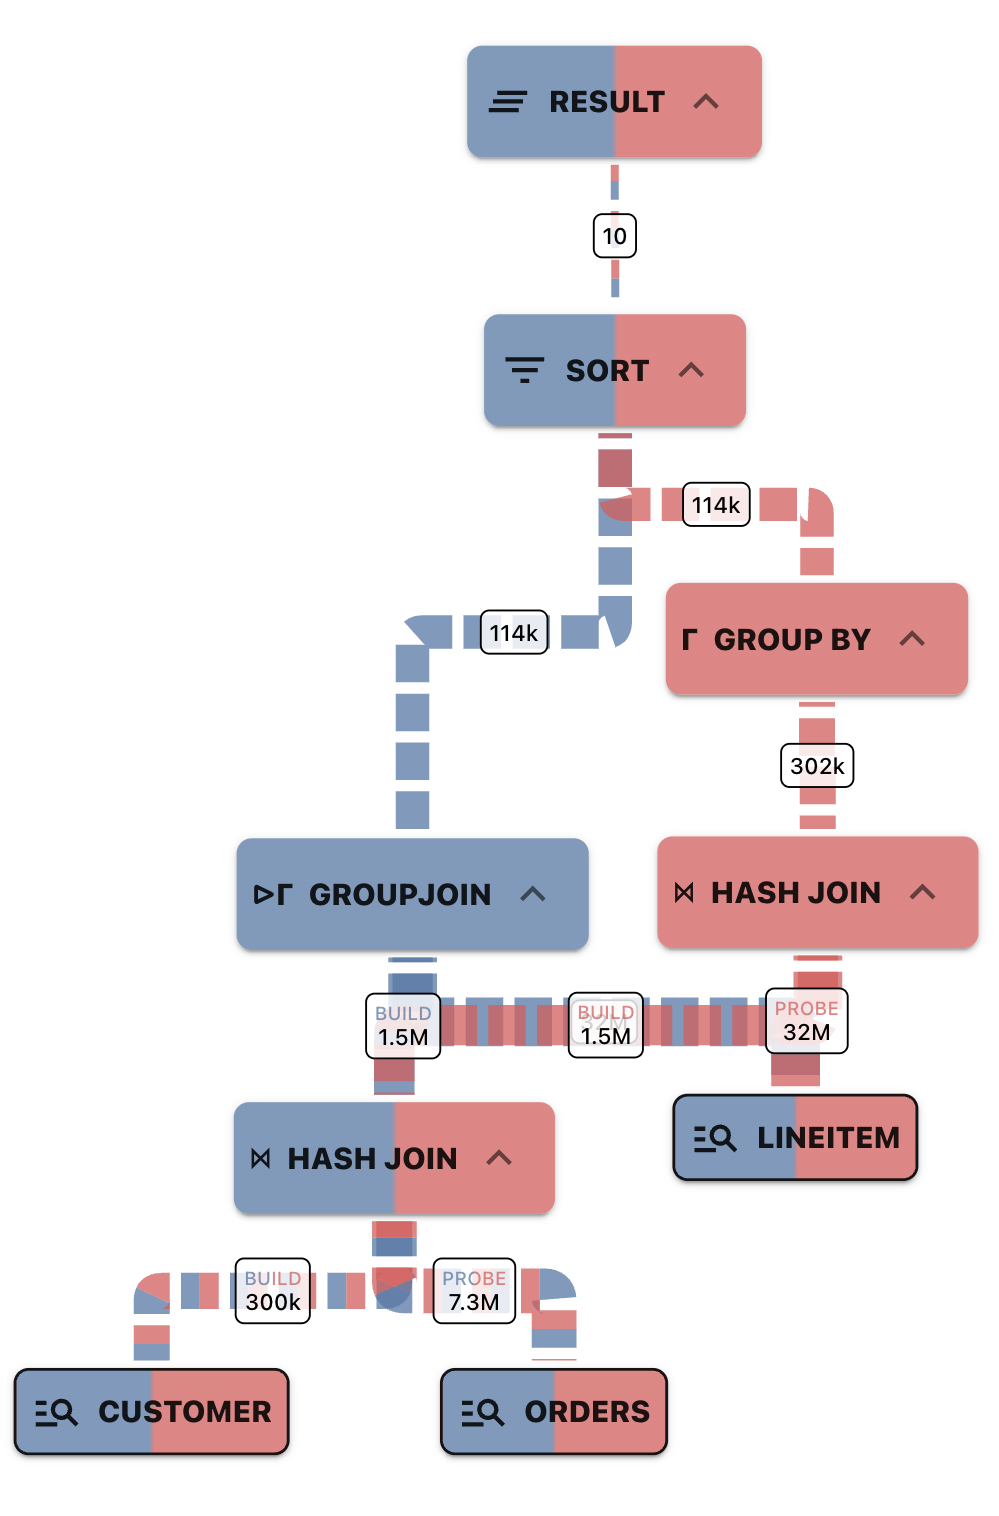
\includegraphics[width=\linewidth]{figures/query-plan-combined-slim.png}
      \caption{Comparison of different query plans, where similar parts are merged together.}
      \label{fig:query-plan-combined}
  \end{subfigure}
  \caption{Query plan comparison between different database systems.}
  \label{fig:query-plan}
\end{figure}


% Funktionen des Query-Plans
The query plan feature is equipped with many tools designed to facilitate a thorough inspection of query plans.
% Combine Trees
A central capability is the merging of all activated query plans using a specified strategy, using the slider illustrated in Figure~\ref{fig:query-plan-slider}. This merging process, exemplified in Figure~\ref{fig:query-plan-combined}, involves summarizing identical subtrees across different plans. Such merging proves invaluable for inspecting divergences in inspected queries, as varying query plan structures are more clearly visualized. For an in-depth exploration of merging strategies, please refer to Section \ref{sec:semantic-diff-integration}.


\begin{figure}[h]
  \centering
  
\includegraphics[width=0.25\linewidth]{figures/query-plan-slider.png}
  \caption{Selection of the query plan merging strategy in the form of a slider.}
  \label{fig:query-plan-slider}
\end{figure}

% Hide Subtree
For extensive query plans, it's beneficial to conceal subtrees that are presently less relevant. This action reduces the overall size of the query plan, emphasizing the more pertinent sections. Users can employ this functionality for any node, as illustrated in Figure~\ref{fig:query-plan-hide-subtree}.

\begin{figure}[h]
  \centering
  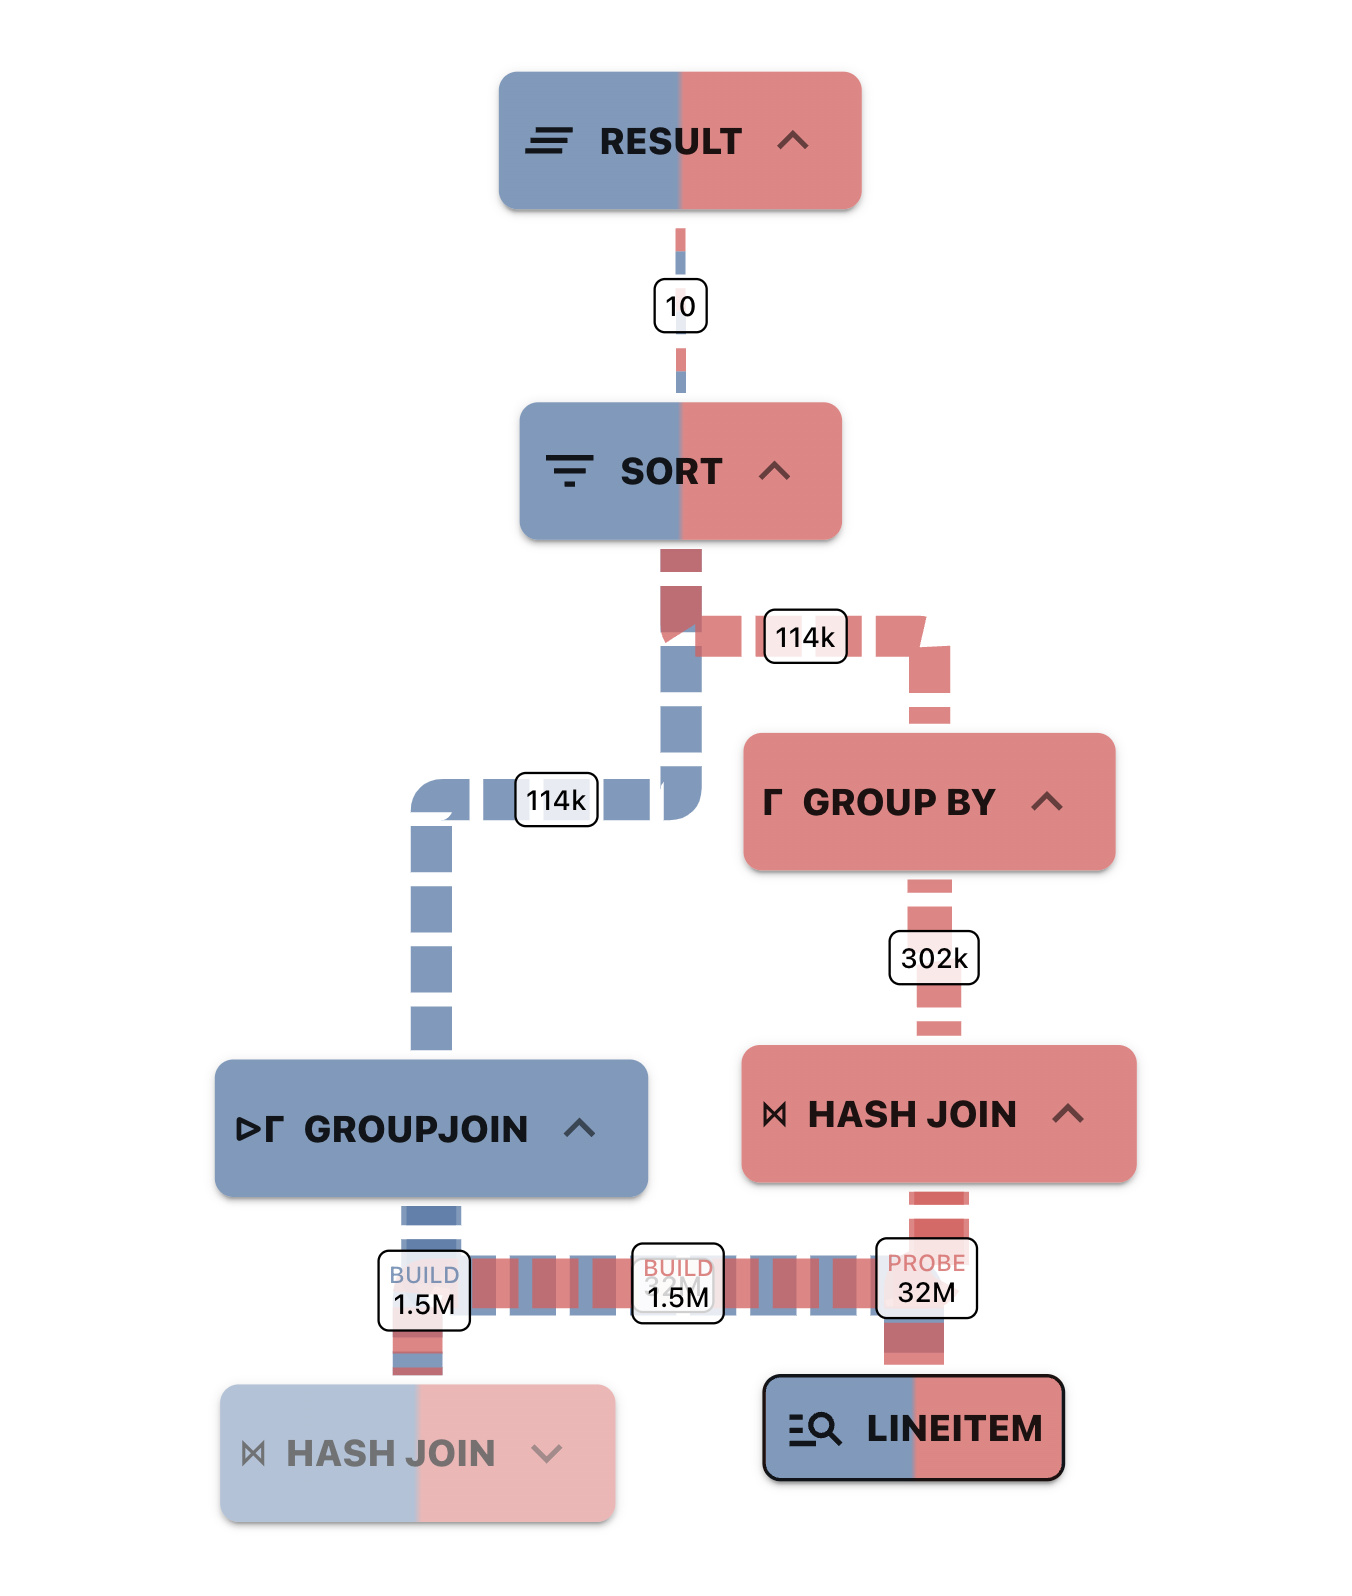
\includegraphics[width=0.35\linewidth]{figures/query-plan-hide-subtree.png}
  \caption{Query plan with a hidden subtree in the bottom left corner.}
  \label{fig:query-plan-hide-subtree}
\end{figure}

% Map
When dealing with extensive query plans, having a tool to comprehend the entire canvas is essential. To facilitate this, a map, as shown in Figure~\ref{fig:query-plan-map}, is included in the bottom right corner of the query plan view. This map provides an overview of the query plans using simplified visual representations of the nodes. Furthermore, it indicates the current location within the complete layout of the query plan, aiding in orientation.

\begin{figure}[h]
  \centering
  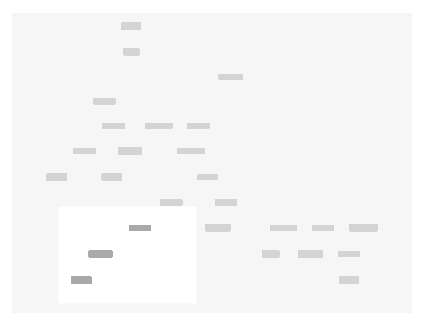
\includegraphics[width=0.25\linewidth]{figures/query-plan-map.png}
  \caption{Map of the query plan showing the current location and the tree in a simplified version.}
  \label{fig:query-plan-map}
\end{figure}

% Node Info, System Representation

The query plan offers supplementary details about nodes. Clicking on a node opens a concise overview, as depicted in Figure~\ref{fig:query-plan-node-info-a}, displaying information about the operator, its type, estimated cardinality, and exact cardinality.\\
In scenarios where multiple databases are activated, and a merged node is selected, the information view shows details for all systems being merged within that node, as illustrated in Figure~\ref{fig:query-plan-node-info-combined}.

\begin{figure}[h]
  \centering
  \begin{subfigure}[b]{0.4\linewidth}
    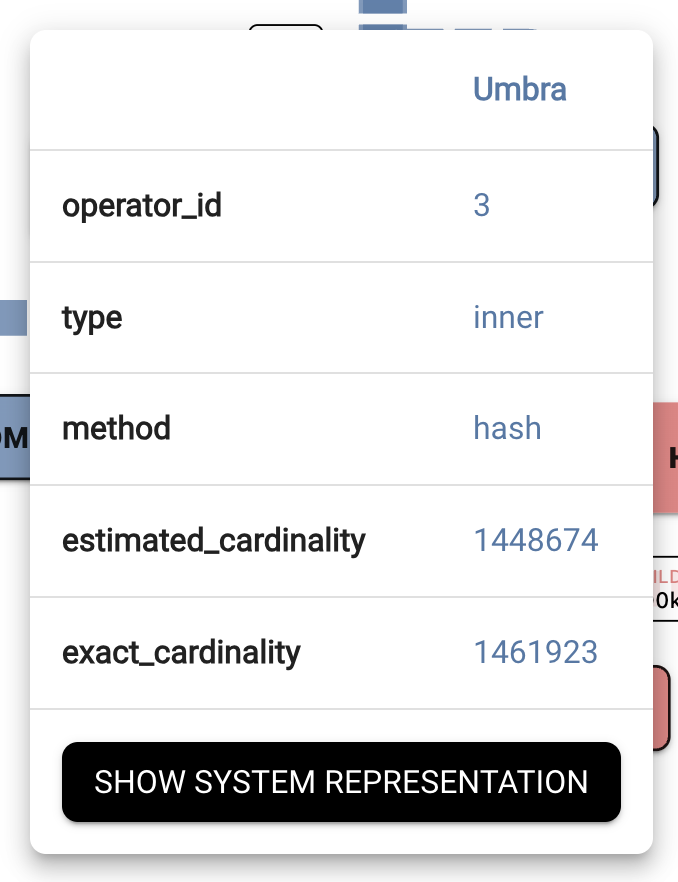
\includegraphics[width=0.7\linewidth]{figures/query-plan-node-info.png}
    \caption{Node information window.}
      \label{fig:query-plan-node-info-a}
  \end{subfigure}
  \hspace{1cm} % Adjust the horizontal space between the figures
  \begin{subfigure}[b]{0.4\linewidth}
      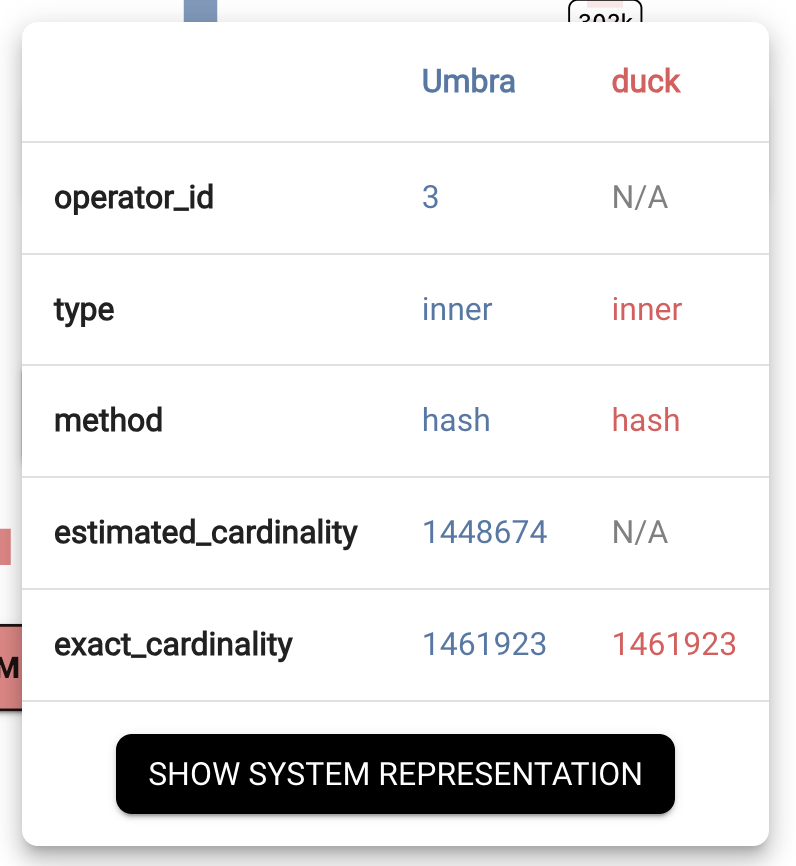
\includegraphics[width=0.8\linewidth]{figures/query-plan-node-info-combined.png}
      \caption{Node information window of a shared node.}
      \label{fig:query-plan-node-info-combined}
  \end{subfigure}
  \caption{Node information window of the selected node.}
  \label{fig:query-plan-node-info}
\end{figure}

The information window also allows displaying the system representation. As an overlay, similar to Figure~\ref{fig:query-plan-system-representation}, the system representation appears in the style of a simple code editor, presenting information in a code-like format. Line numbers are displayed on the left, and an overview of the file is shown on the right.

\begin{figure}[h]
  \centering
  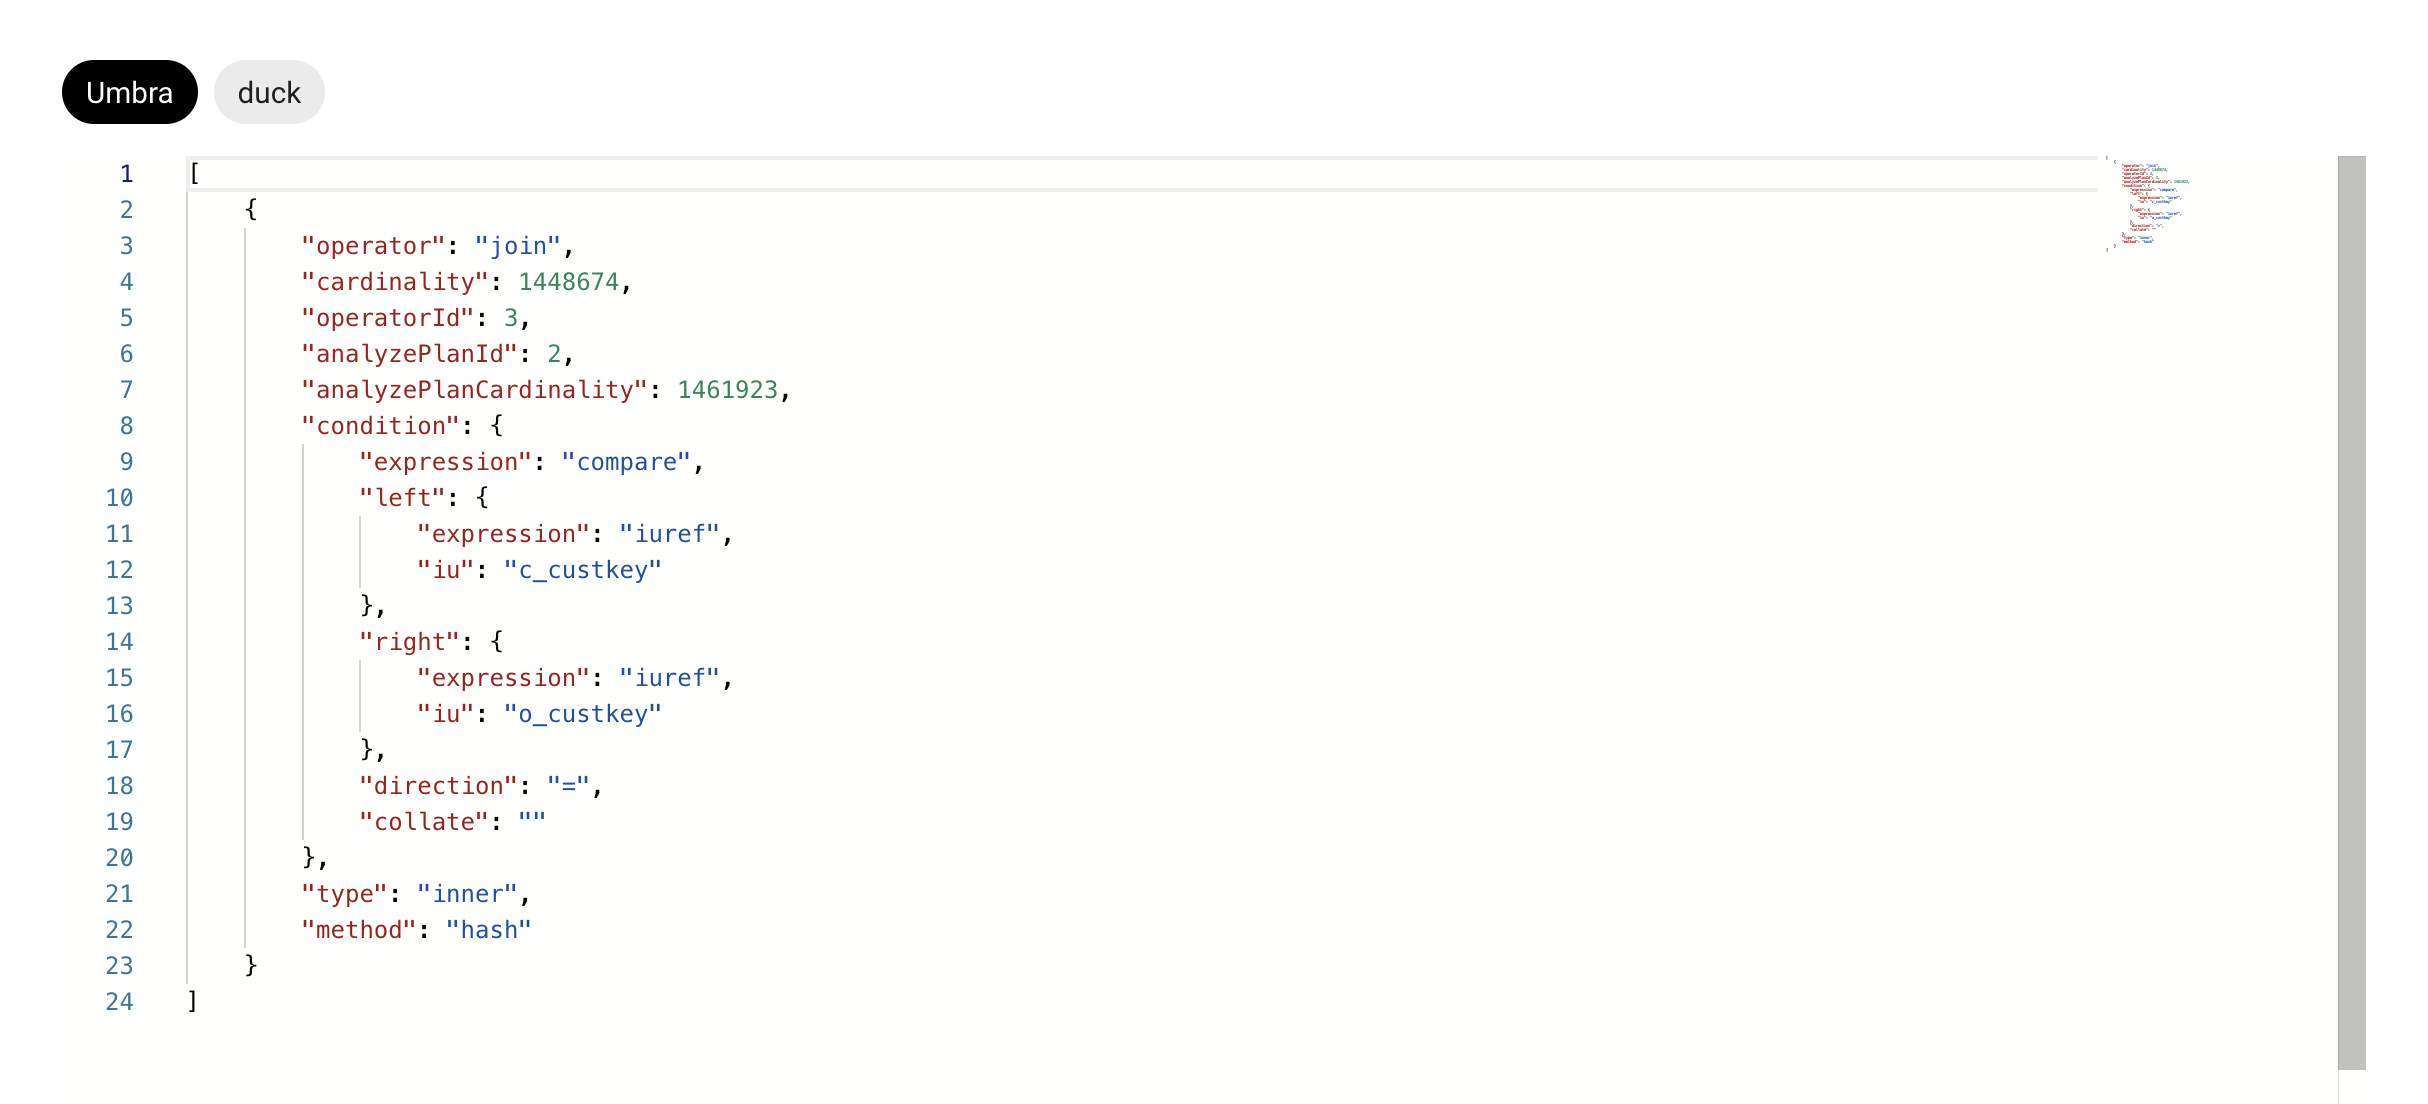
\includegraphics[width=0.8\linewidth]{figures/query-plan-node-system-representation-combined.png}
  \caption{Query plan system representaion of a node.}
  \label{fig:query-plan-system-representation}
\end{figure}

At the top, the user can choose the database system for which the system representation should be displayed in the case of a merged node.

All these functionalities are provided by the standalone application Query Plan Visualizer \parencite*{semantic-diff}. We dive deeper into the integration of the semantic diff tool in the section \ref{sec:semantic-diff-integration}.


\subsection{Flexible Interface Hub}

To offer a well-suited platform for analyzing specific performance differences of high complexity, a flexible system is essential for conducting these analytical processes. Such flexibility is crucial for providing tailored solutions to inspect specific aspects of benchmark data.

In this section, we will explore how the Benchy Viewer achieves this functionality, primarily through a drag-and-drop system for visualization elements. This empowers users to select the necessary visualizations and construct a comprehensive overview.

Subsequently, we will delve deeper into the actual visualizations, examining the flexibility of configuring charts and plots to optimize the perspective of performance data within a specific visualization.

\subsubsection{Drag and Drop}
The drag-and-drop system integrated into the Benchy Viewer empowers users to effortlessly rearrange every chart and plot. Beyond the flexibility offered by individual visualization elements, users can strategically organize visualizations within containers. These containers are essentially thematic sections, each represented by a headline. Users have the flexibility to rename these containers, creating dedicated spaces for specific topics and populating them with relevant charts and plots.

\begin{figure}[h]
  \centering
  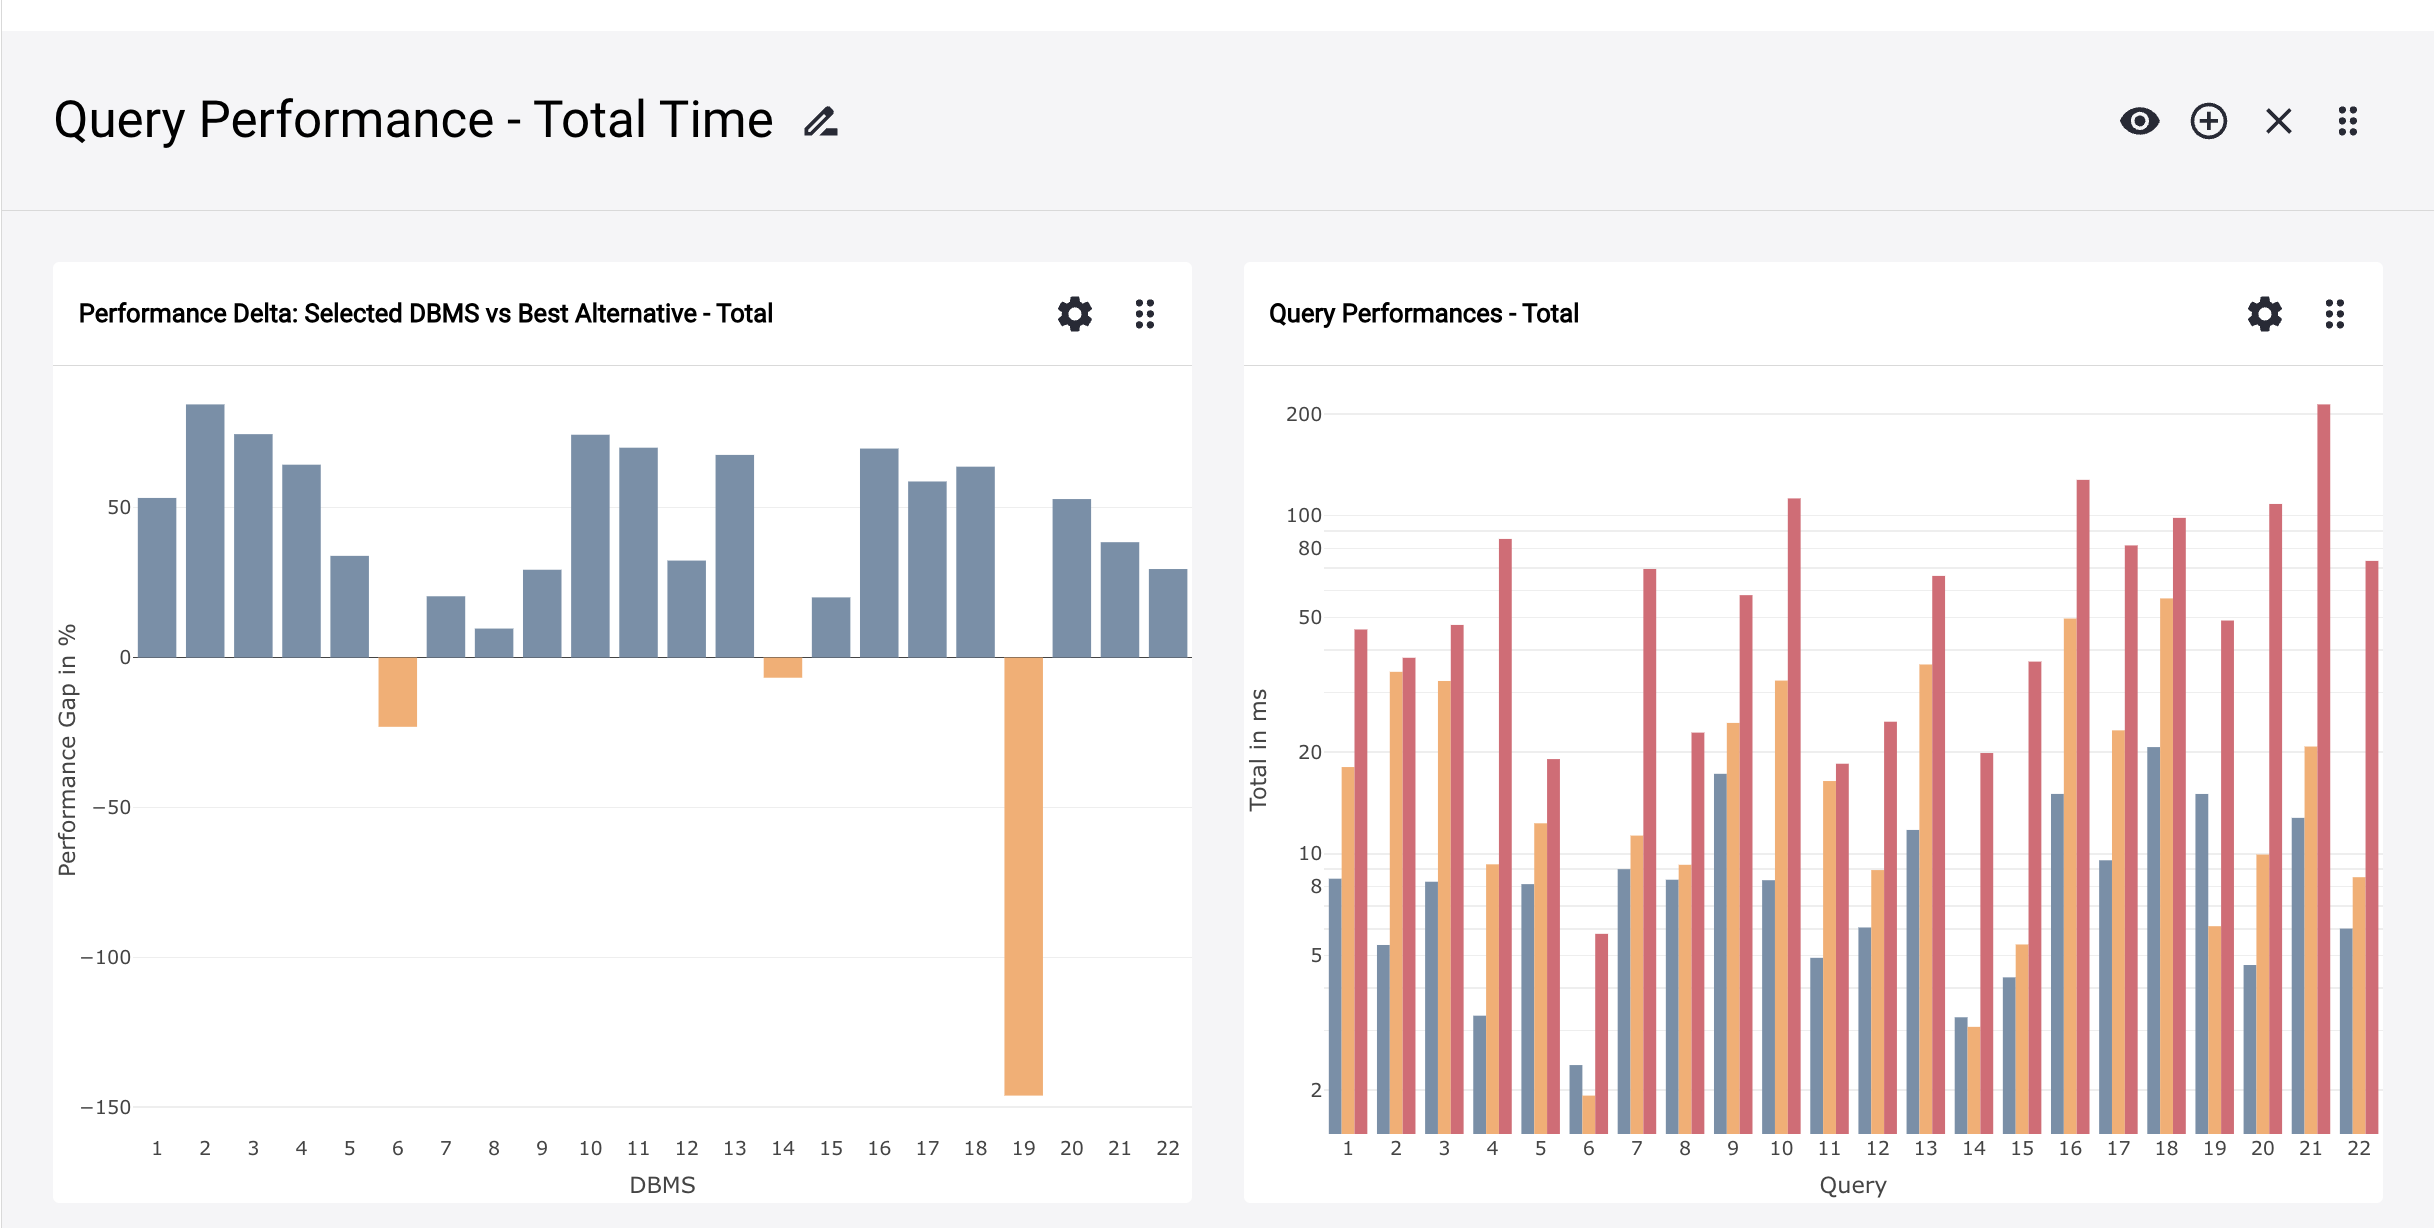
\includegraphics[width=0.8\linewidth]{figures/analytics-drag-and-drop.png}
  \caption{Flexible interface hub through drag-and-drop feature for visualization elements and their containers.}
  \label{fig:analytics-drag-and-drop}
\end{figure}

The versatility of containers allows them to function as distinct analytical sections, housing visualization elements pertinent to that specific context. Moreover, the dynamic nature of the Benchy Viewer enables users to seamlessly move visualizations between containers, fostering adaptability in organizing and categorizing data. The ability to drag entire containers further enhances this adaptability, enabling users to arrange sections according to their analytical preferences. This dual flexibility, within containers and with container placement, provides users with a robust framework for tailoring their analytical environment to meet the demands of diverse datasets.

\subsubsection{Analytics Sections}

% Rename Section
The top header of a container, as illustrated in Figure~\ref{fig:analytics-drag-and-drop}, serves as a hub for fundamental container functionalities. An intuitive feature allows users to rename a container by clicking on the edit icon situated next to the container's label. This action triggers a dialogue with a straightforward text input, as depicted in Figure~\ref{fig:analytics-section-rename}. Once users input and confirm the new label using the "ok" button, the container's label promptly updates.\\
Users can now efficiently organize and contextualize their analytical elements within appropriately named containers. The ability to swiftly modify container labels enhances the user experience, enabling them to maintain a well-structured and easily navigable analytical workspace.

\begin{figure}[h]
  \centering
  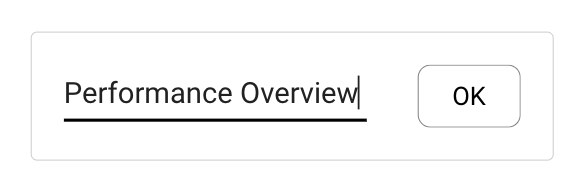
\includegraphics[width=0.25\linewidth]{figures/analytics-section-rename.png}
  \caption{Text input for renaming containers.}
  \label{fig:analytics-section-rename}
\end{figure}

% Add chart
To enrich the content within a container, users can effortlessly incorporate charts and plots using the icon positioned in the right corner of the container's header. This action opens an overlay menu presenting a variety of available plots and charts for inclusion in the container, as showcased in Figure~\ref{fig:analytics-add-chart}. Upon the user's selection of a visualization element, the analytical section promptly updates, seamlessly integrating the chosen element into its content.

\begin{figure}[h]
  \centering
  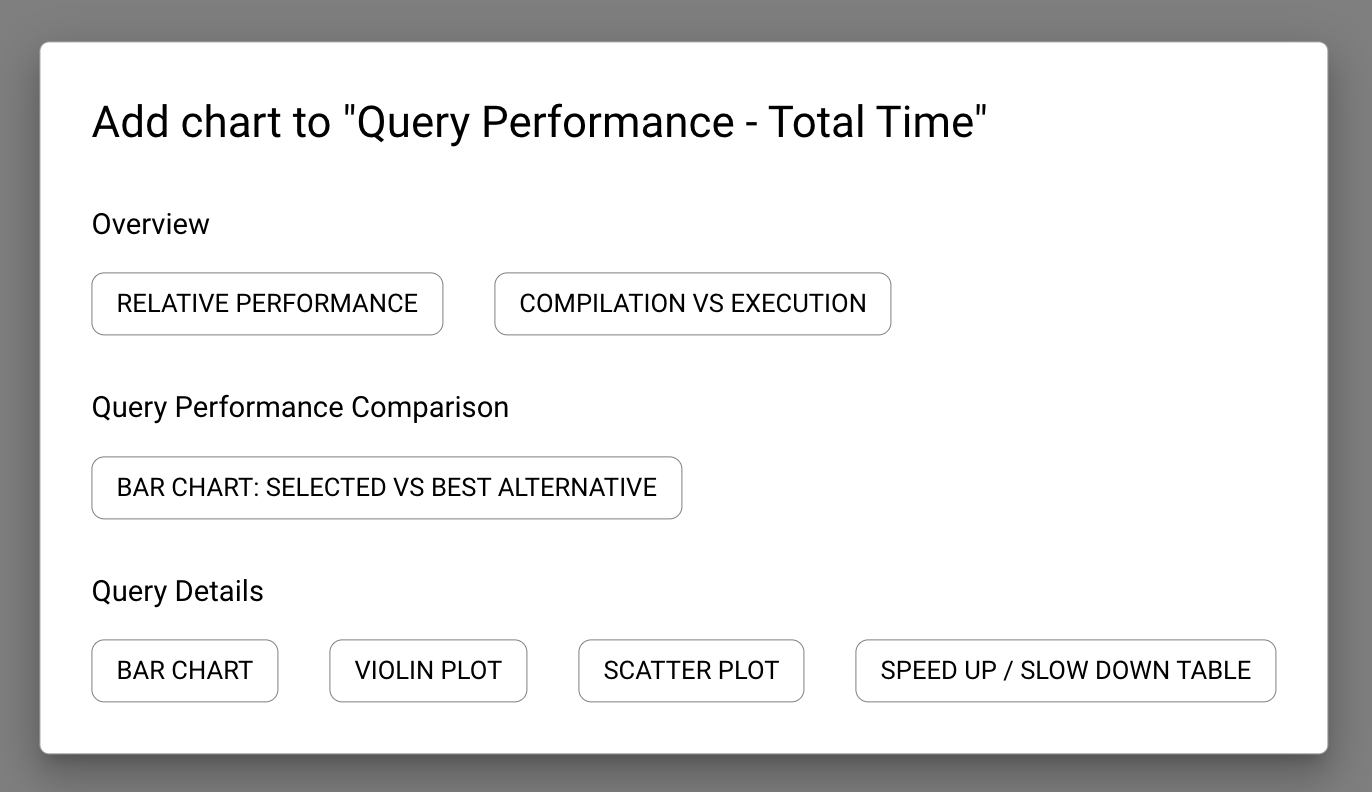
\includegraphics[width=0.6\linewidth]{figures/analytics-add-chart.png}
  \caption{Overlay for adding charts to the current container.}
  \label{fig:analytics-add-chart}
\end{figure}

This intuitive process streamlines the augmentation of analytical sections, allowing users to dynamically enhance their workspace with relevant visualizations. The added charts and plots are instantly ready for utilization, fostering a fluid and responsive analytical environment within the Benchy Viewer.\\
We dive deeper into the utilization and configuration of the charts and plots in \ref{sec:chart-configuration}.


% Set Visibility of containers
Another valuable functionality in the container's header is the visibility toggle. Users can swiftly conceal an analytics section by simply clicking the visibility icon of a container, as illustrated in Figure~\ref{fig:analytics-section-visibility}. This action disables the view of the content, revealing only the header of the container. Users can easily reactivate visibility or access other functionalities.

\begin{figure}[h]
  \centering
  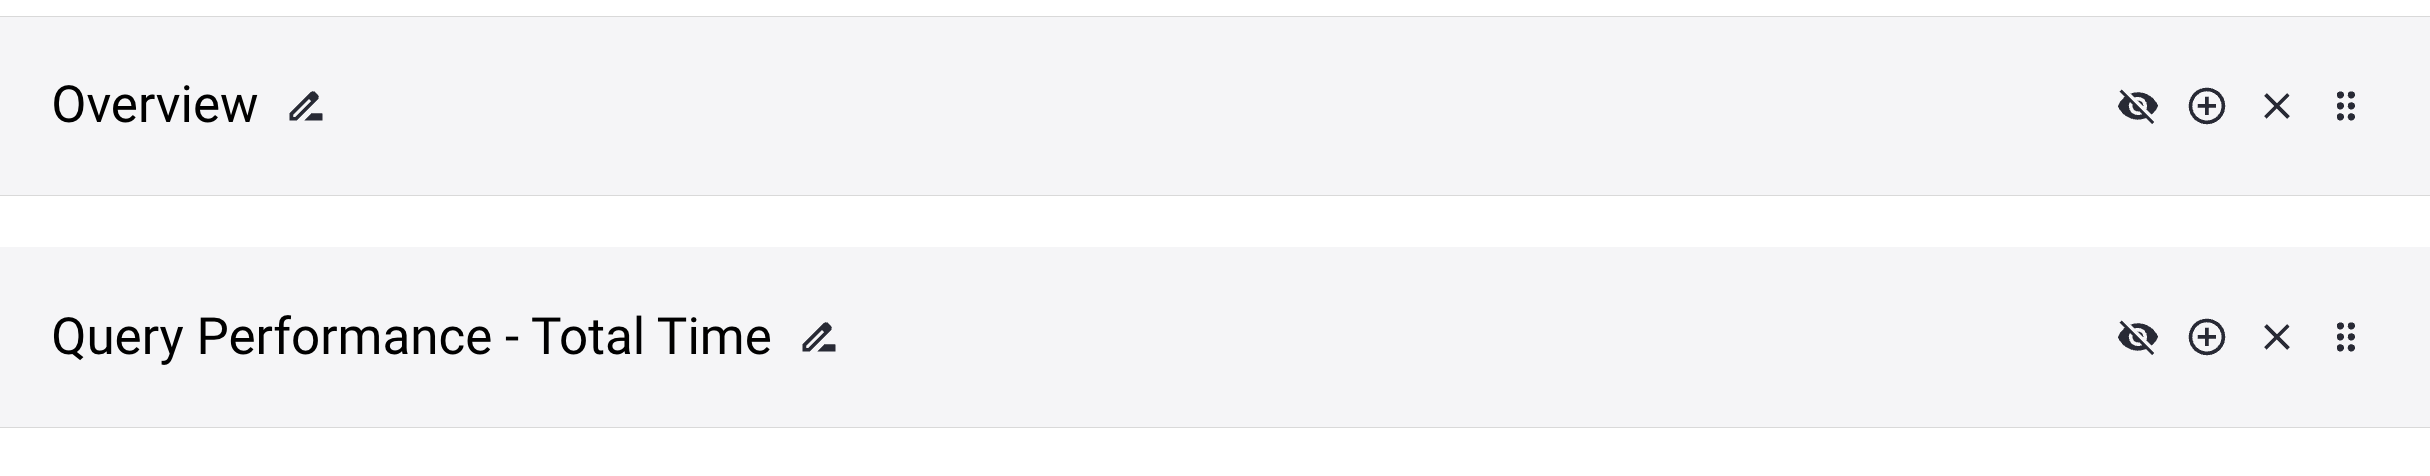
\includegraphics[width=0.8\linewidth]{figures/analytics-section-visibility.png}
  \caption{Visibility property to hide or expand a container.}
  \label{fig:analytics-section-visibility}
\end{figure}

The convenience of collapsing containers, coupled with the drag-and-drop feature, enhances overall user comfort and efficiency. This uncomplicated feature significantly enhances clarity and ease of use, especially when managing a substantial number of visualizations and diverse data perspectives.

Initiating the deletion process, another noteworthy feature embedded in the container's header is the delete function. By clicking on the delete icon of a container, users can efficiently remove an analytics section. This action permanently eliminates the container and its content. This straightforward delete function provides a quick and effective way to manage the organizational structure of visualizations.


\subsubsection{Chart Configurations}\label{sec:chart-configuration}

Within the Benchy Viewer, a versatile dashboard serves as a backdrop for seamless interaction with diverse visualizations. Delving into individual visualization elements, the platform prioritizes adaptability, allowing users to tailor charts and plots to their specific requirements.\\
We'll explore the capability to select a metric within a chart, demonstrate the flexibility of switching to a table visualization in the context of maximum speedup and maximum slowdown, and finally, highlight global chart options.

\begin{figure}[h]
  \centering
  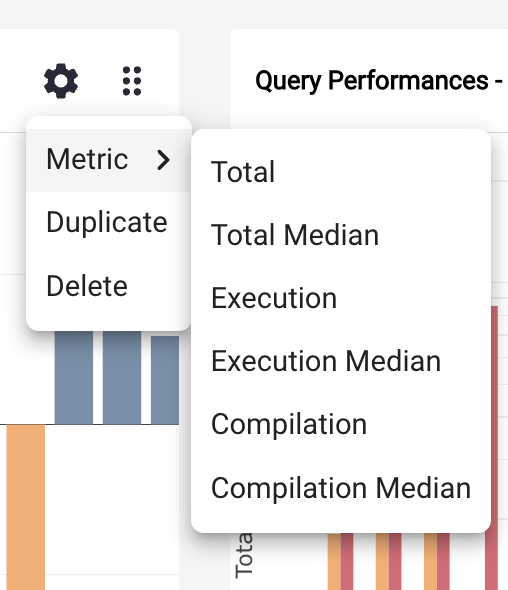
\includegraphics[width=0.35\linewidth]{figures/chart-configuration.png}
  \caption{Drop-down menu of chart options offering to select the visualized metric. Also the delete and duplicate functionality is provided.}
  \label{fig:chart-configuration}
\end{figure}

% - Metrics auswählen
Every visualization element within the drag-and-drop dashboard features a header, as illustrated in Figure~\ref{fig:analytics-drag-and-drop}. Beyond the drag-and-drop functionality, the header hosts an options icon, providing access to various configuration settings, as depicted in Figure~\ref{fig:chart-configuration}.\\
Within the nested drop-down menu, users can seamlessly tailor their selection of metrics to meet specific needs.

Upon selecting a metric, the chart dynamically updates, presenting the new data within the current visualization framework. This rapid and flexible construction of charts enhances the user's ability to gain valuable insights swiftly.

Similarly, users can quickly duplicate a chart for comparative analysis or delete it to streamline the dashboard. The duplicate function allows for the replication of a chart with its current settings, providing an efficient way to explore variations of the same data.\\
Conversely, the delete function promptly removes a chart, contributing to a clutter-free and focused visual workspace. These functionalities collectively empower users to fine-tune their analytical environment for a seamless exploration experience.

% - tabele und scatter: speedup/ slowdown
In the analytical process of working with the metric pair speedup and slowdown, seamlessly toggling between maximum speedup and maximum slowdown is crucial. The Benchy Viewer facilitates this transition through the switch icon integrated into the header of the table visualization, as exemplified in Figure~\ref{fig:chart-configuration-table-switch}.

\begin{figure}[h]
  \centering
  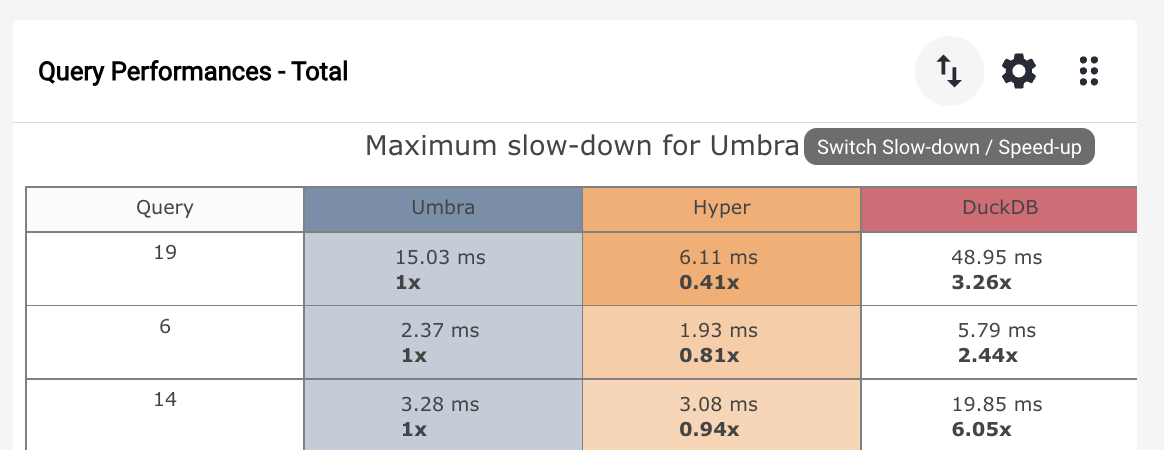
\includegraphics[width=0.8\linewidth]{figures/chart-configuration-table-switch.png}
  \caption{Table visualization provides the functionality to switch between maximum speedup and maximum slowdown.}
  \label{fig:chart-configuration-table-switch}
\end{figure}

A simple click on the switch icon triggers the table to transition to the alternate mode, dynamically updating its data to reflect the chosen metric. This feature ensures a fluid and efficient exploration of performance data, allowing users to effortlessly switch between speedup and slowdown perspectives as needed.


% - Scale: Linear/ Log/ Throuput
In addition to the nuanced control over individual visualizations, the Benchy Viewer empowers users with global chart options, allowing users to sculpt the visual landscape to their specific analytical requirements.

One of the noteworthy features is the ability to globally switch the Y-axis type, as depicted in Figure~\ref{fig:chart-configuration-scale}. This flexibility allows users to choose between linear, logarithmic, and throughput representations, offering diverse perspectives on the benchmark data. Whether aiming for a detailed examination of variations in lower values or emphasizing proportional changes, the global Y-axis type switch ensures that the visualizations align with the user's analytical focus.

\begin{figure}[h]
  \centering
  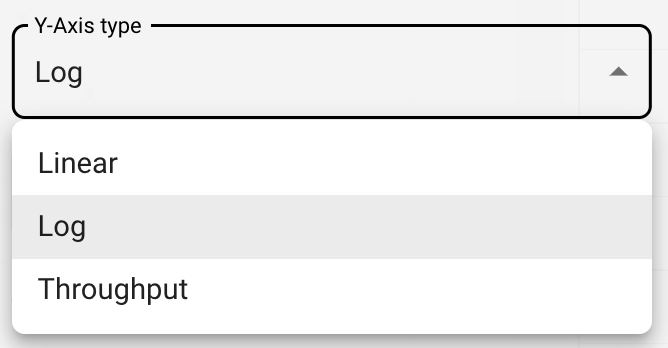
\includegraphics[width=0.3\linewidth]{figures/chart-configuration-scale.png}
  \caption{Drop-down menu of global options offering the selection of the scale type.}
  \label{fig:chart-configuration-scale}
\end{figure}

The linear scale is ideal when a precise examination of small variations in data is paramount. This scale excels in offering a detailed, granular view, particularly advantageous for closely positioned metric values.

\begin{figure}[h]
  \centering
  \begin{subfigure}[b]{0.3\linewidth}
    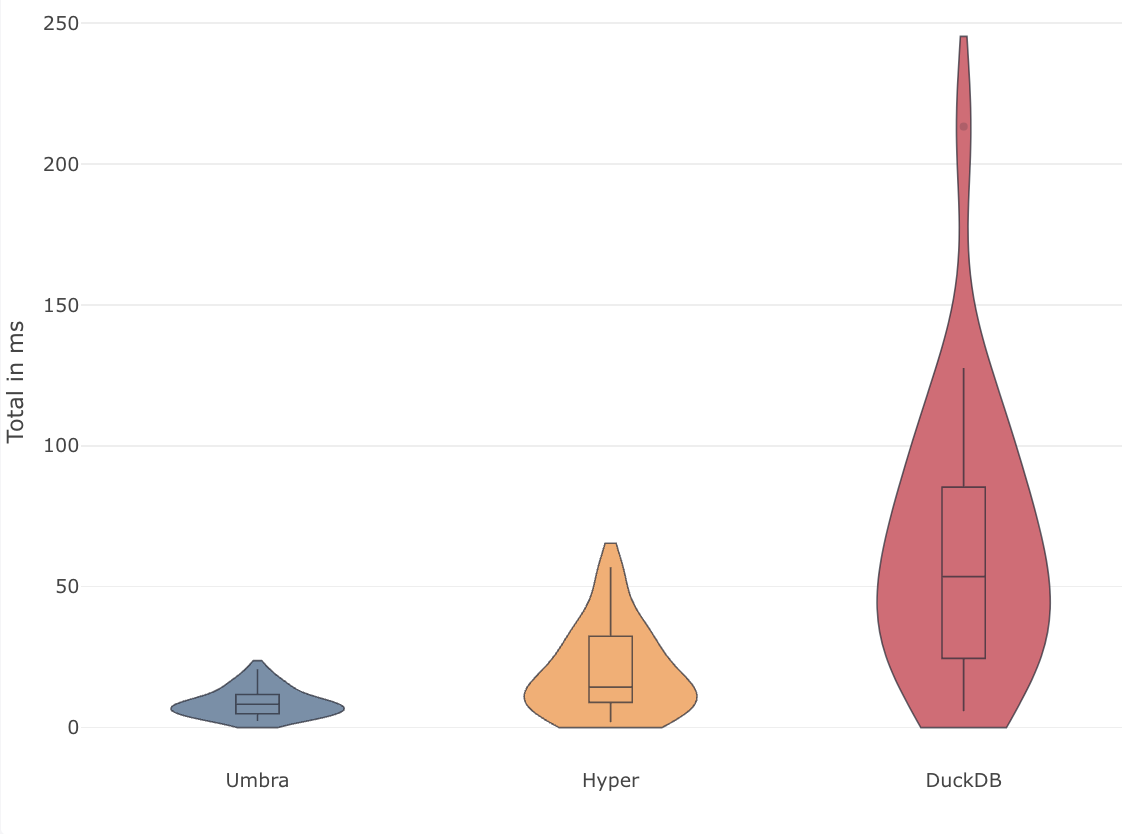
\includegraphics[width=\linewidth]{figures/scale-linear.png}
    \caption{Violin plot with linear scale.}
      \label{fig:scale-linear}
  \end{subfigure}
  \hspace{0.5cm} % Adjust the horizontal space between the figures
  \begin{subfigure}[b]{0.3\linewidth}
    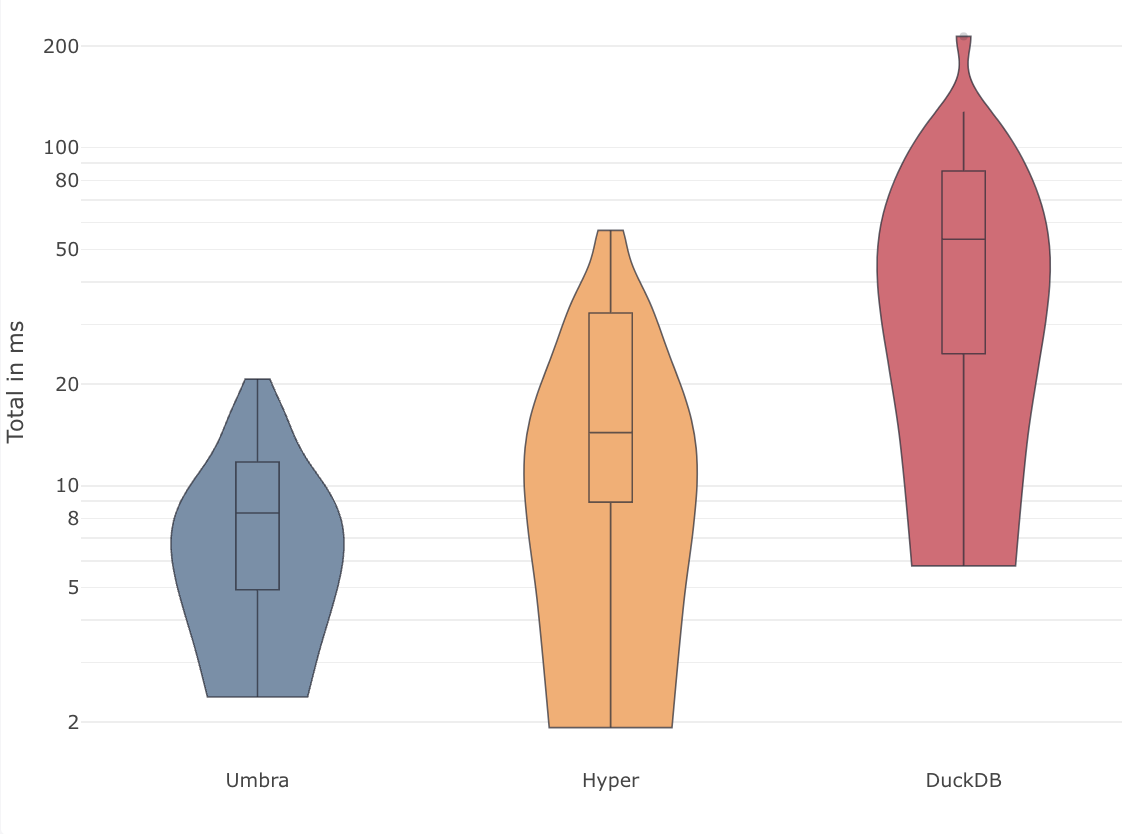
\includegraphics[width=\linewidth]{figures/scale-log.png}
    \caption{Violin plot with logarithmic scale.}
      \label{fig:scale-log}
  \end{subfigure}
  \hspace{0.5cm} % Adjust the horizontal space between the figures
  \begin{subfigure}[b]{0.3\linewidth}
    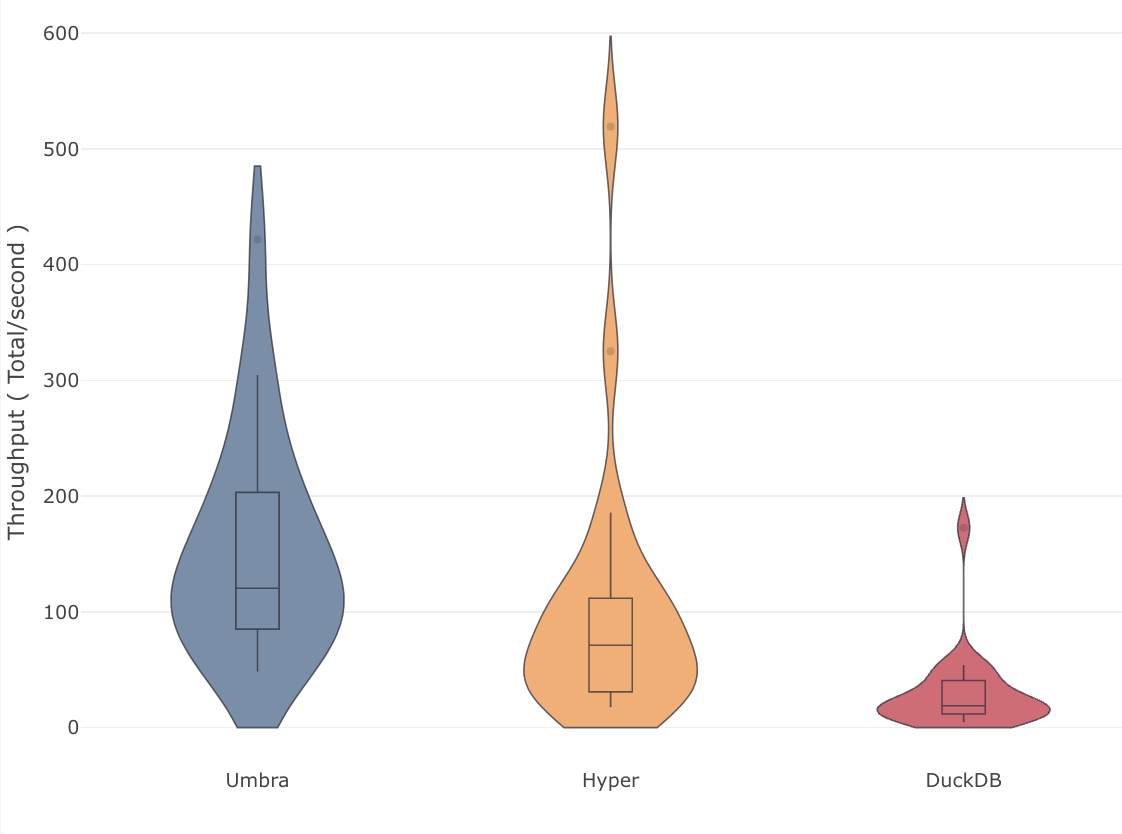
\includegraphics[width=\linewidth]{figures/scale-throughput.png}
    \caption{Violin plot with throughput based scale.}
      \label{fig:scale-throughput}
  \end{subfigure}
  \caption{Comparison of violin plots using different scales: A visual representation of the same dataset, highlighting how variations appear under linear, logarithmic, and throughput scaling.}
  \label{fig:scale-comparison.}
\end{figure}

The logarithmic scale excels in highlighting proportional changes across a wide range of values. This is particularly advantageous when dealing with datasets that span several orders of magnitude, ensuring that both small and large values are perceptible.

The throughput scale is specifically designed for scenarios where the emphasis is on the rate of data transfer or processing. It provides a unique perspective, crucial in benchmarking scenarios where throughput is a critical performance metric.

By seamlessly switching between these Y-axis types globally, users can extract diverse insights from the same set of data, enhancing the versatility and depth of their analytical processes.


% - Violin: scatter und boxplot
The Benchy Viewer also offers customization options for violin plots. Users can choose between representing data inside the violins as individual data points or as a boxplot, as illustrated in Figure~\ref{fig:chart-configuration-violin}. Opting for data points means that each query data is individually represented, providing a wealth of detailed information. On the other hand, selecting the "Boxplot" option replaces individual data points with a summarized boxplot inside the violin. This option streamlines the visualization, offering clarity by presenting an overview of the data distribution. Users have the flexibility to tailor the representation based on their specific analytical needs.

\begin{figure}[h]
  \centering
  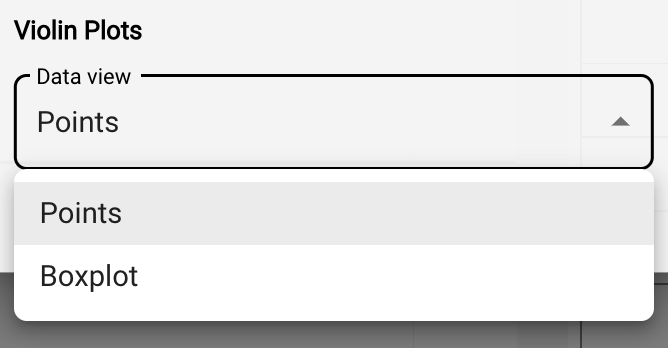
\includegraphics[width=0.4\linewidth]{figures/chart-configuration-violin.png}
  \caption{Drop-down menu of global options, offering the selection of displaying data points or a boxplot within the violins of the violin charts.}
  \label{fig:chart-configuration-violin}
\end{figure}

\subsection{Saving and Sharing the Application State}\label{sec:saving-sharing-state}

One of the valuable features of the Benchy Viewer is its ability to save and share the application state. This encompasses all configurations related to visualization elements, global options, and dashboard settings. Users can conveniently save their current setup or download it for future reference, as depicted in Figure~\ref{fig:save-upload}.

\subsubsection{Downloading Configuration}
The saved configurations can be downloaded as a file, allowing users to keep a record of specific setups or share them with colleagues. This downloaded file serves as a snapshot of the application state at the time of saving.

\subsubsection{Uploading Configurations}
To recreate a previous analysis session, users can upload a saved configuration file. This action loads all the configurations, restoring the dashboard layout, applied visualizations, and global settings. It's a time-saving feature that ensures a seamless transition back to a specific analytical context.


\begin{figure}[h]
  \vspace{0.5cm}
  \centering
  
\includegraphics[width=0.4\linewidth]{figures/save-upload.png}
  \caption{Downloading and uploading the application state.}
  \label{fig:save-upload}
\end{figure}


\subsubsection{Facilitating Collaboration}
The ability to share configuration files promotes collaboration among users. Team members can easily exchange analysis setups, ensuring a consistent view of data and enabling more effective collaboration on complex analytical projects.

In essence, the "Saving and Sharing" feature enhances the flexibility and collaborative potential of the Benchy Viewer, providing users with a convenient way to exchange analytical contexts.

% !TeX root = ../main.tex
% Add the above to each chapter to make compiling the PDF easier in some editors.

\section{Design}
In this section, we explore the foundational principles guiding the Benchy Viewer's user interface. Rooted in Material Design, the application employs Material UI components for a clean and familiar look. The deliberate color scheme, restricted to black, white, and gray accents, promotes simplicity.

Moving on, we delve into the sidebar and the header, ensuring constant visibility and facilitating seamless navigation. The sidebar acts as a central hub, offering functionalities from page navigation to data import. The header contains crucial elements like the legend, eliminating the need for one in each visualization.

Finally, we examine the application's pages: Analytics Dashboard, Query Plan View, and Input File View. Each serves a distinct purpose, from analysing benchmark data to offering a minimalist view of raw imported data. 


\subsection{User Interface Design Styles}
\subsubsection{Material UI}
% MUI Zitate 
% sx Style Properties
The Benchy Viewer's design is rooted in the principles of Material Design\textcolor{red}{Zitat}, emphasizing a sleek and consistent user interface that aligns with modern design standards.\\
To ensure a cohesive and user-centric design, the application makes extensive use of predefined components from the Material UI framework. This includes buttons, inputs, toggles, sliders, data grids, icons, drop-down menus, and tooltips.

The inclusion of Material Design components contributes to an interface that is both user-friendly and familiar. Users can easily navigate through buttons, toggles, and sliders, thanks to the standardized styling that Material UI provides.

Icons within the Benchy Viewer serve as visual cues, representing familiar symbols that aid users in quickly grasping the functions they perform. This visual clarity aligns with Material Design's emphasis on intuitive iconography.

Settings options, presented in dropdown menus and other interfaces, follow Material Design practices. The design prioritizes user intuition, allowing individuals to interact with the application seamlessly without relying on extensive textual explanations.

By aligning with Material Design principles, the Benchy Viewer achieves a design that not only meets aesthetic standards, but also prioritizes user understanding and interaction efficiency. The incorporation of familiar components enhances the overall usability and accessibility of the application.


\subsubsection{Styling Characteristics}

The Benchy Viewer embraces a deliberate color scheme aimed at providing a clean design. This is achieved through a restraint to specific base colors, limiting the palette to black, white, and a gray accent color, as depicted in Figure~\ref{fig:colors}. By adhering to this minimalist approach, the application exudes a sense of simplicity, ensuring a visually uncluttered interface.



\begin{figure}[h]
  \centering
  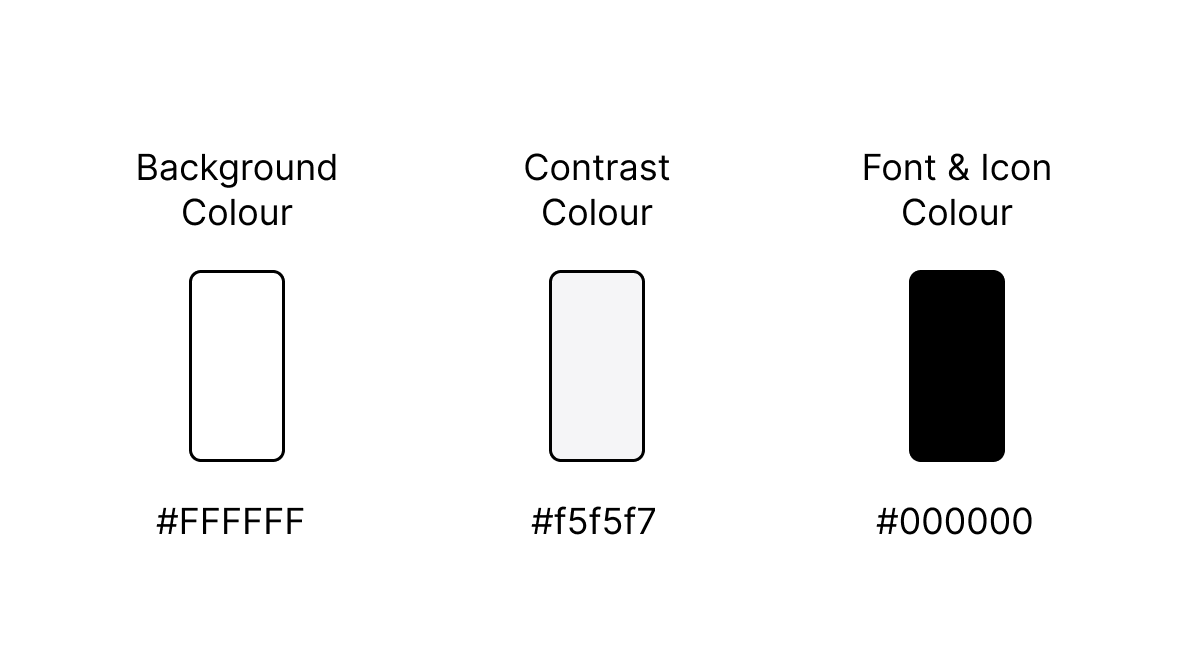
\includegraphics[width=0.4\linewidth]{figures/colors.png}
  \caption{Color palette of the user interface.}
  \label{fig:colors}
\end{figure}

While the overall design adheres to a subdued color palette, the visual elements within the application utilize a distinct color scheme, as illustrated in Figure~\ref{fig:colors-dbms}. This strategic approach guarantees that charts, plots, and other visual elements command attention, supporting users to focus on those data visualizations.

\begin{figure}[h]
  \centering
  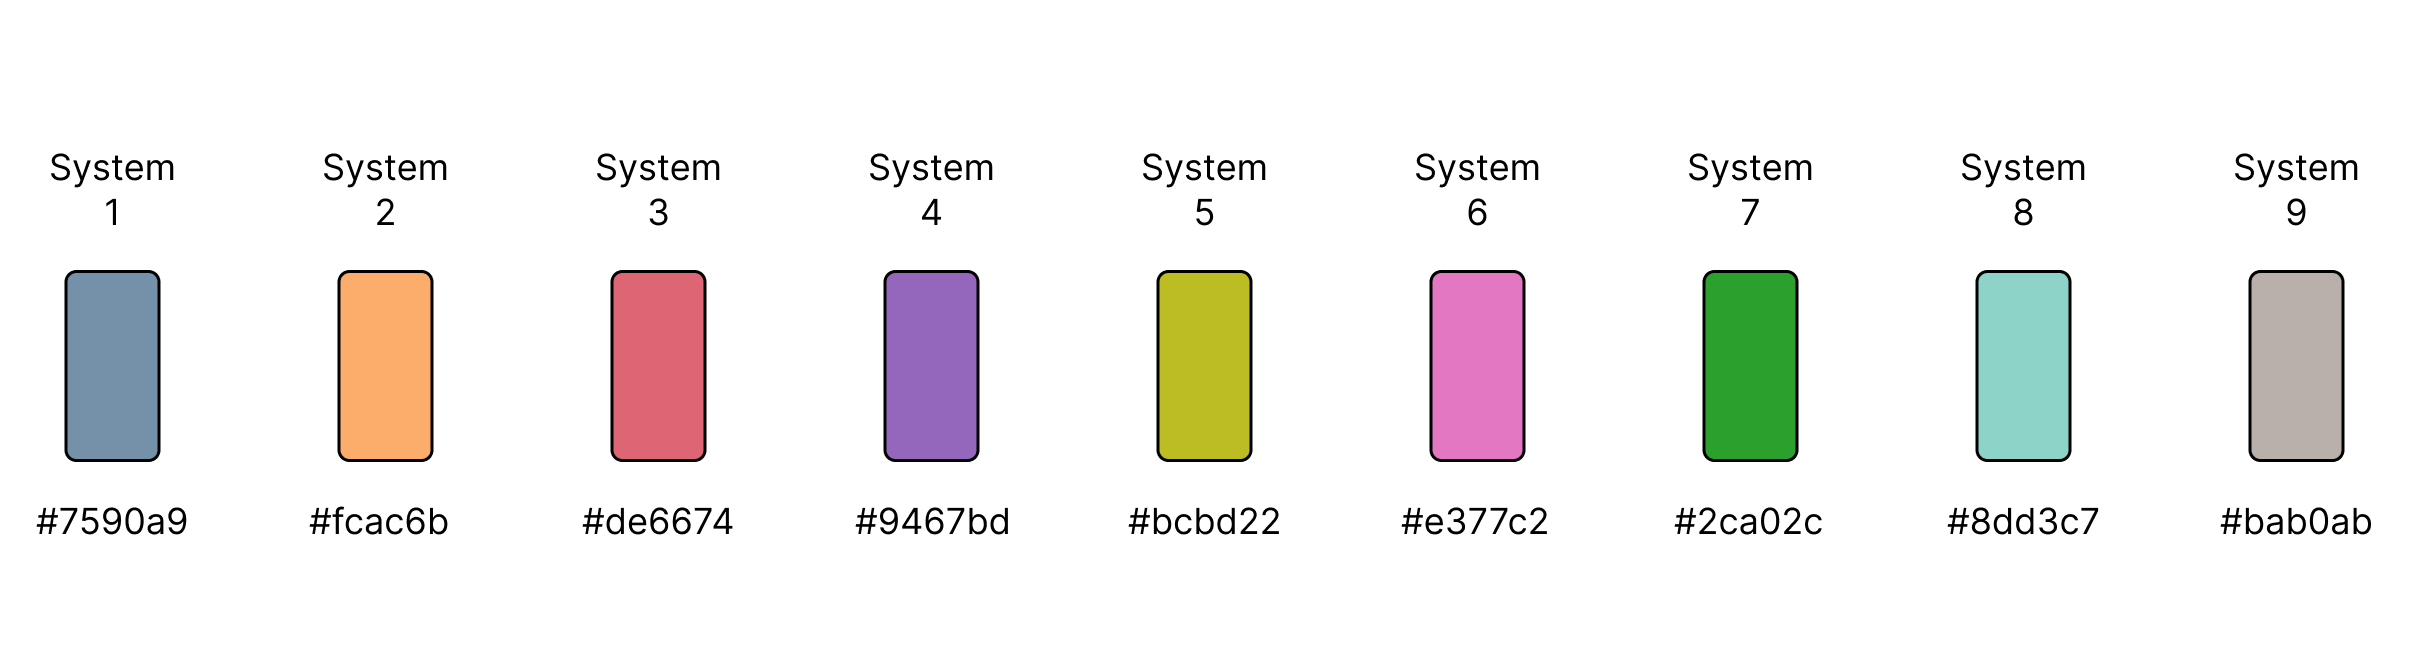
\includegraphics[width=1\linewidth]{figures/colors-dbms.png}
  \caption{Color palette used by visualizations.}
  \label{fig:colors-dbms}
\end{figure}

To enhance user experience, the Benchy Viewer incorporates immediate feedback mechanisms. When users hover over interactive elements, such as buttons or inputs, accent colors dynamically adjust, providing a visual cue of the interactive nature of the element. Additionally, the mouse representation undergoes subtle changes, reinforcing the responsiveness of the interface.\\
Additionally, the Benchy Viewer employs the Roboto font \textcolor{red}{Zitat} for a clean and modern look, enhancing readability and contributing to a user-friendly interface.


\subsection{Page Structure and Navigation}\label{sec:page-structure}

The design of the Benchy Viewer is thoughtfully crafted for user convenience and simplicity. This section provides insights into the structural components that define the organization of the Benchy Viewer.

At the heart of the application's architecture are the header and the sidebar, ensuring constant visibility for users and facilitating seamless navigation. These elements contribute to maintaining a strong sense of orientation throughout the user journey.


\subsubsection{Sidebar}

The Benchy Viewer adopts a standard web view with a sidebar, leveraging the familiar layout seen in many web applications, as illustrated in Figure~\ref{fig:app}. This approach comes with inherent advantages. Users accustomed to web interfaces will find this structure intuitive and easily navigable, contributing to a seamless user experience.

\begin{figure}[h]
  \centering
  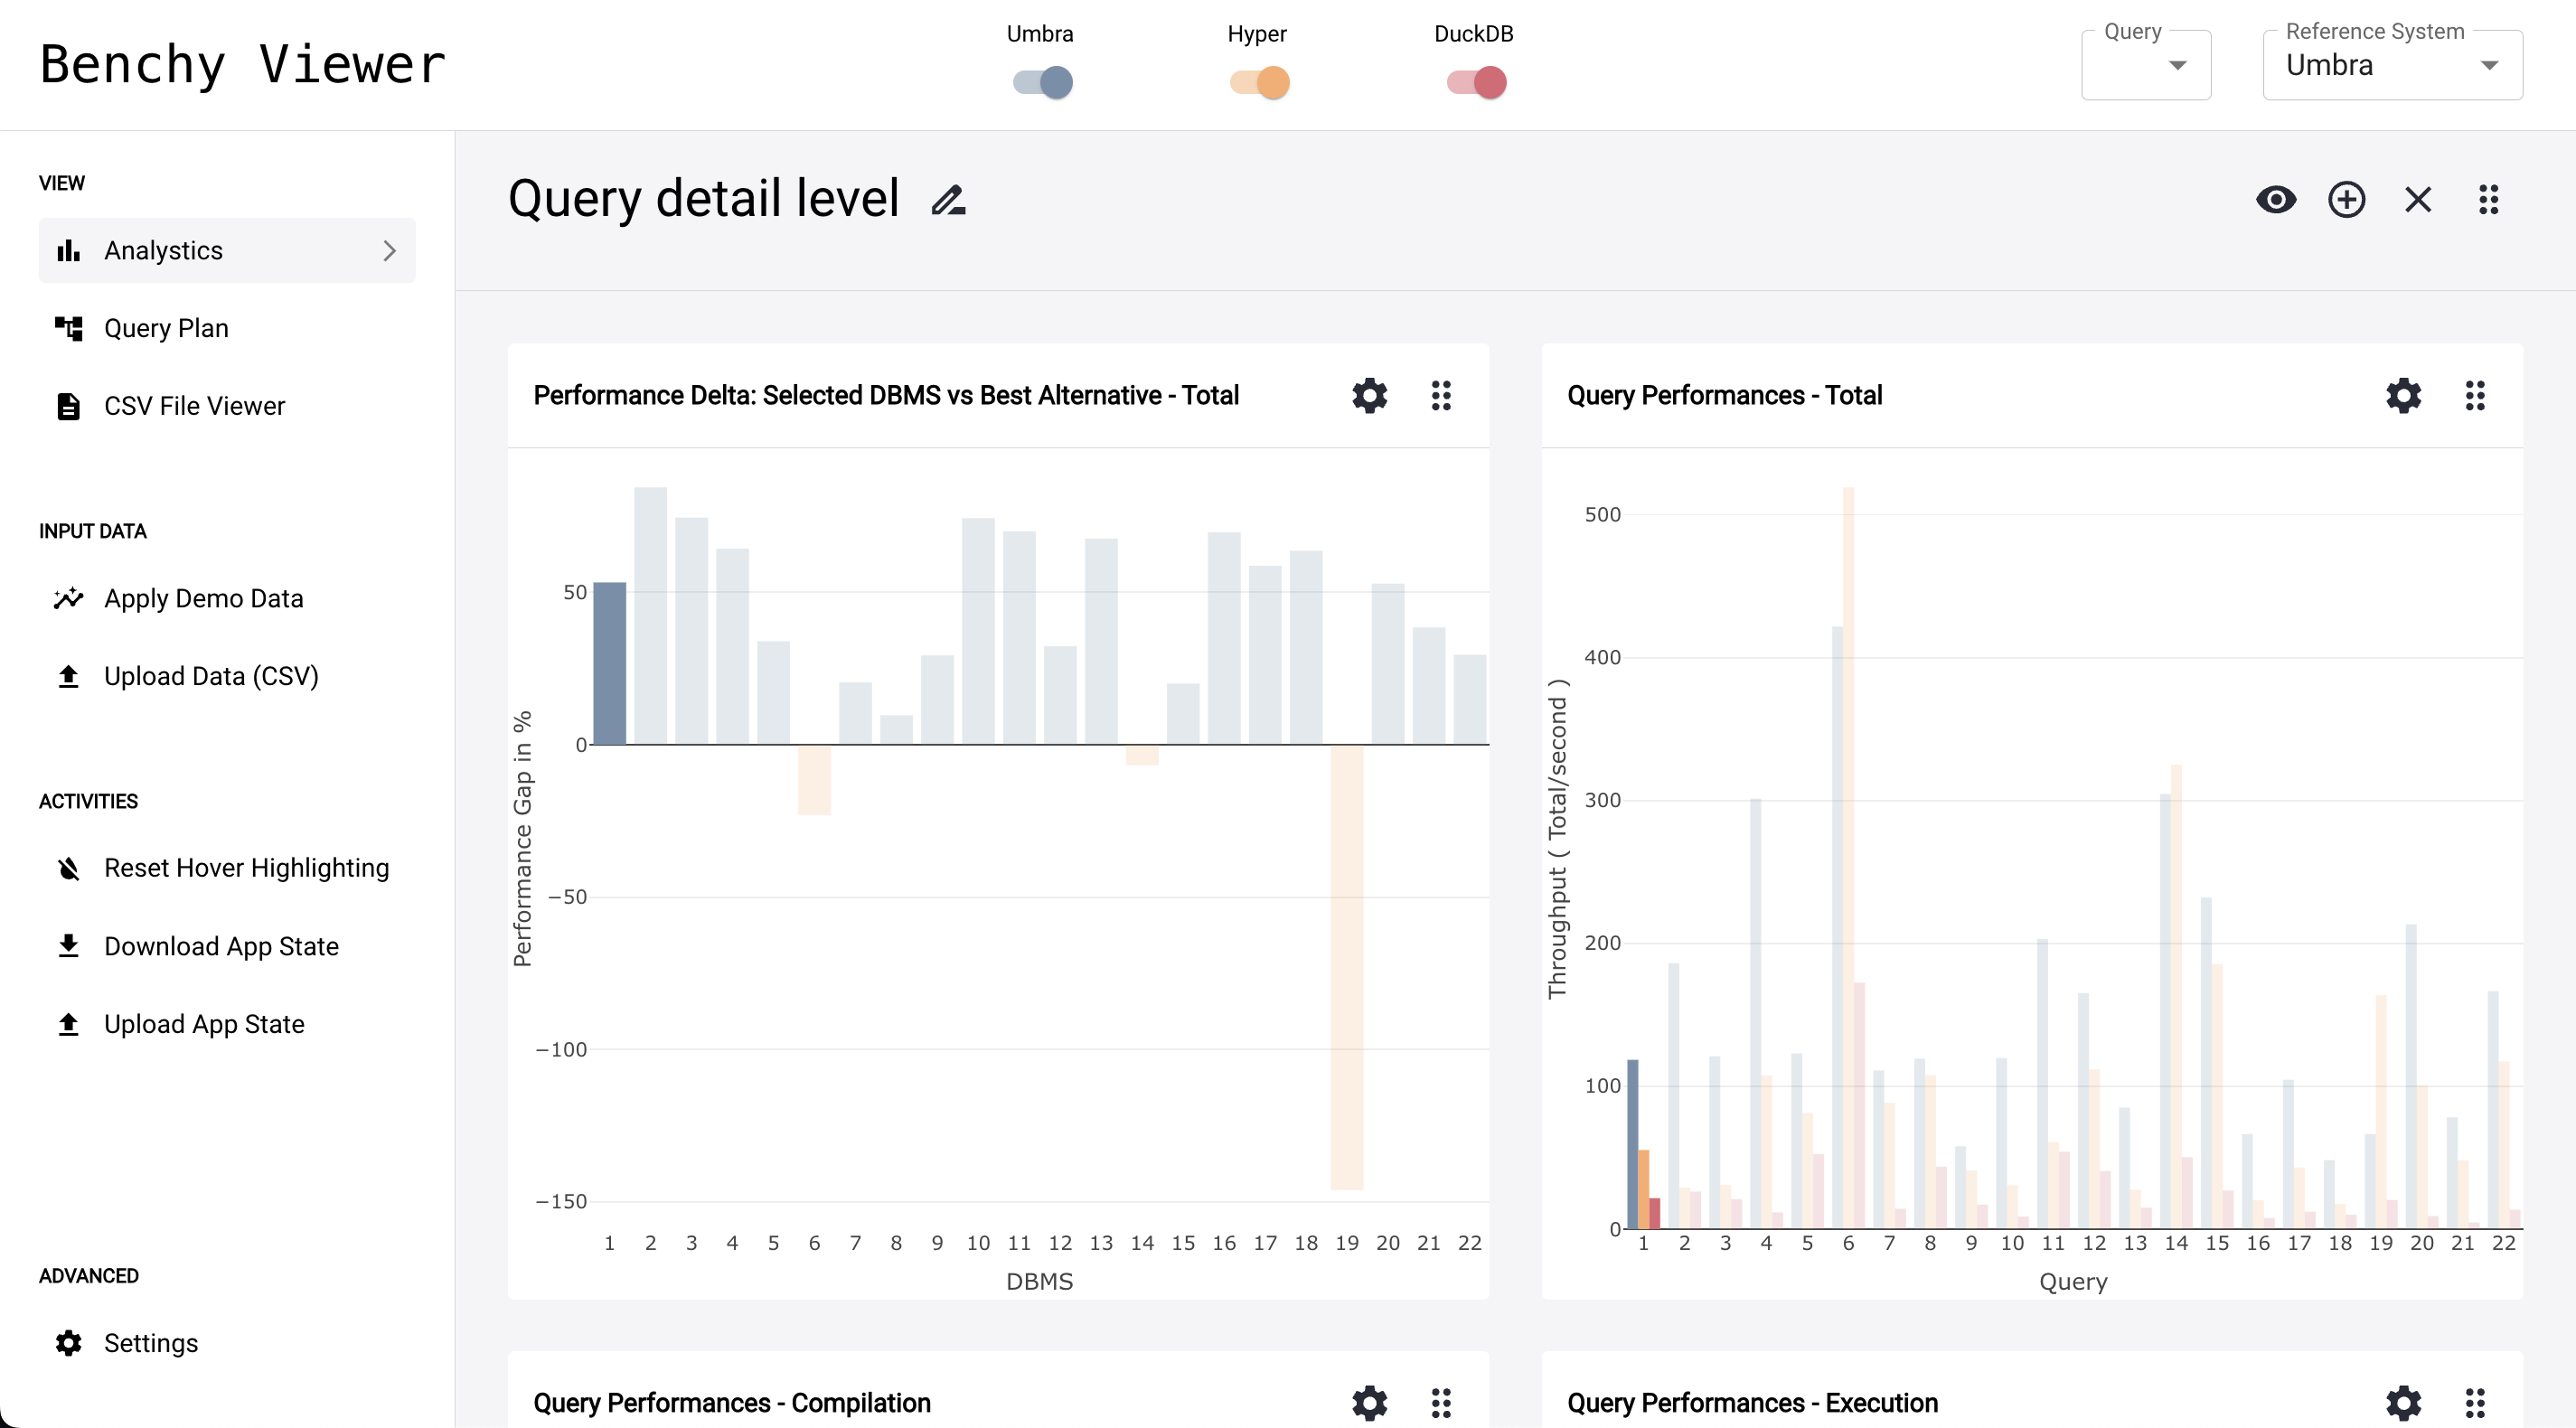
\includegraphics[width=1\linewidth]{figures/app.png}
  \caption{Overview of the application structure.}
  \label{fig:app}
\end{figure}

The sidebar serves as the central hub for navigating different sections of the application, while always staying present. By providing dedicated buttons, users can effortlessly transition between pages, ensuring quick access to specific functionalities and data views. Additionally, the navigation button of the current page is highlighted with the accent color.

Below, the users have the possibility to import benchmark data or explore the application's capabilities using demo data. This feature facilitates a hands-on experience without the immediate need to provide personal datasets, making it convenient for users to evaluate the application's functionalities.

The sidebar offers additional functionalities, including the ability to reset hover highlighting. Users can download and upload the application state, enabling them to save configurations and share them or reload them for future sessions, which is further examined in \ref{sec:saving-sharing-state}. 

A settings icon button in the sidebar provides direct access to the global settings of the Benchy Viewer, allowing users to adjust application-wide settings from anywhere within the application.



\subsubsection{Header}
The header, along with the sidebar, remains visible in all scenarios within the Benchy Viewer. While the sidebar offers a range of functionalities, the header contains fewer elements. The central element of the header is the legend, strategically placed to eliminate the need for a legend in each individual visualization, promoting a clean and efficient overview. Users can activate or deactivate any system at any time using the toggles within the legend.

Another crucial functionality in the header is the selection of the baseline system and the focused query, offering the same advantage of accessibility at any point in the user's workflow.

Additionally, the header adapts contextually when navigating to the "Query Plan" page. In this scenario, a slider appears for selecting the comparison strategy between query plans, providing further flexibility and control, as explored in Section \ref{sec:semantic-diff-integration}.



\subsubsection{Pages}

The Sidebar and Header form the foundation of the user interface, while the remaining space is dedicated to displaying the various pages. Essentially, the Benchy Viewer comprises three main pages, depicted in Figure~\ref{fig:pages}: the Analytics Dashboard page, the Query Plan page, and the Input File Viewer page.

\begin{figure}[h]
  \centering
  \begin{subfigure}[b]{0.3\linewidth}
    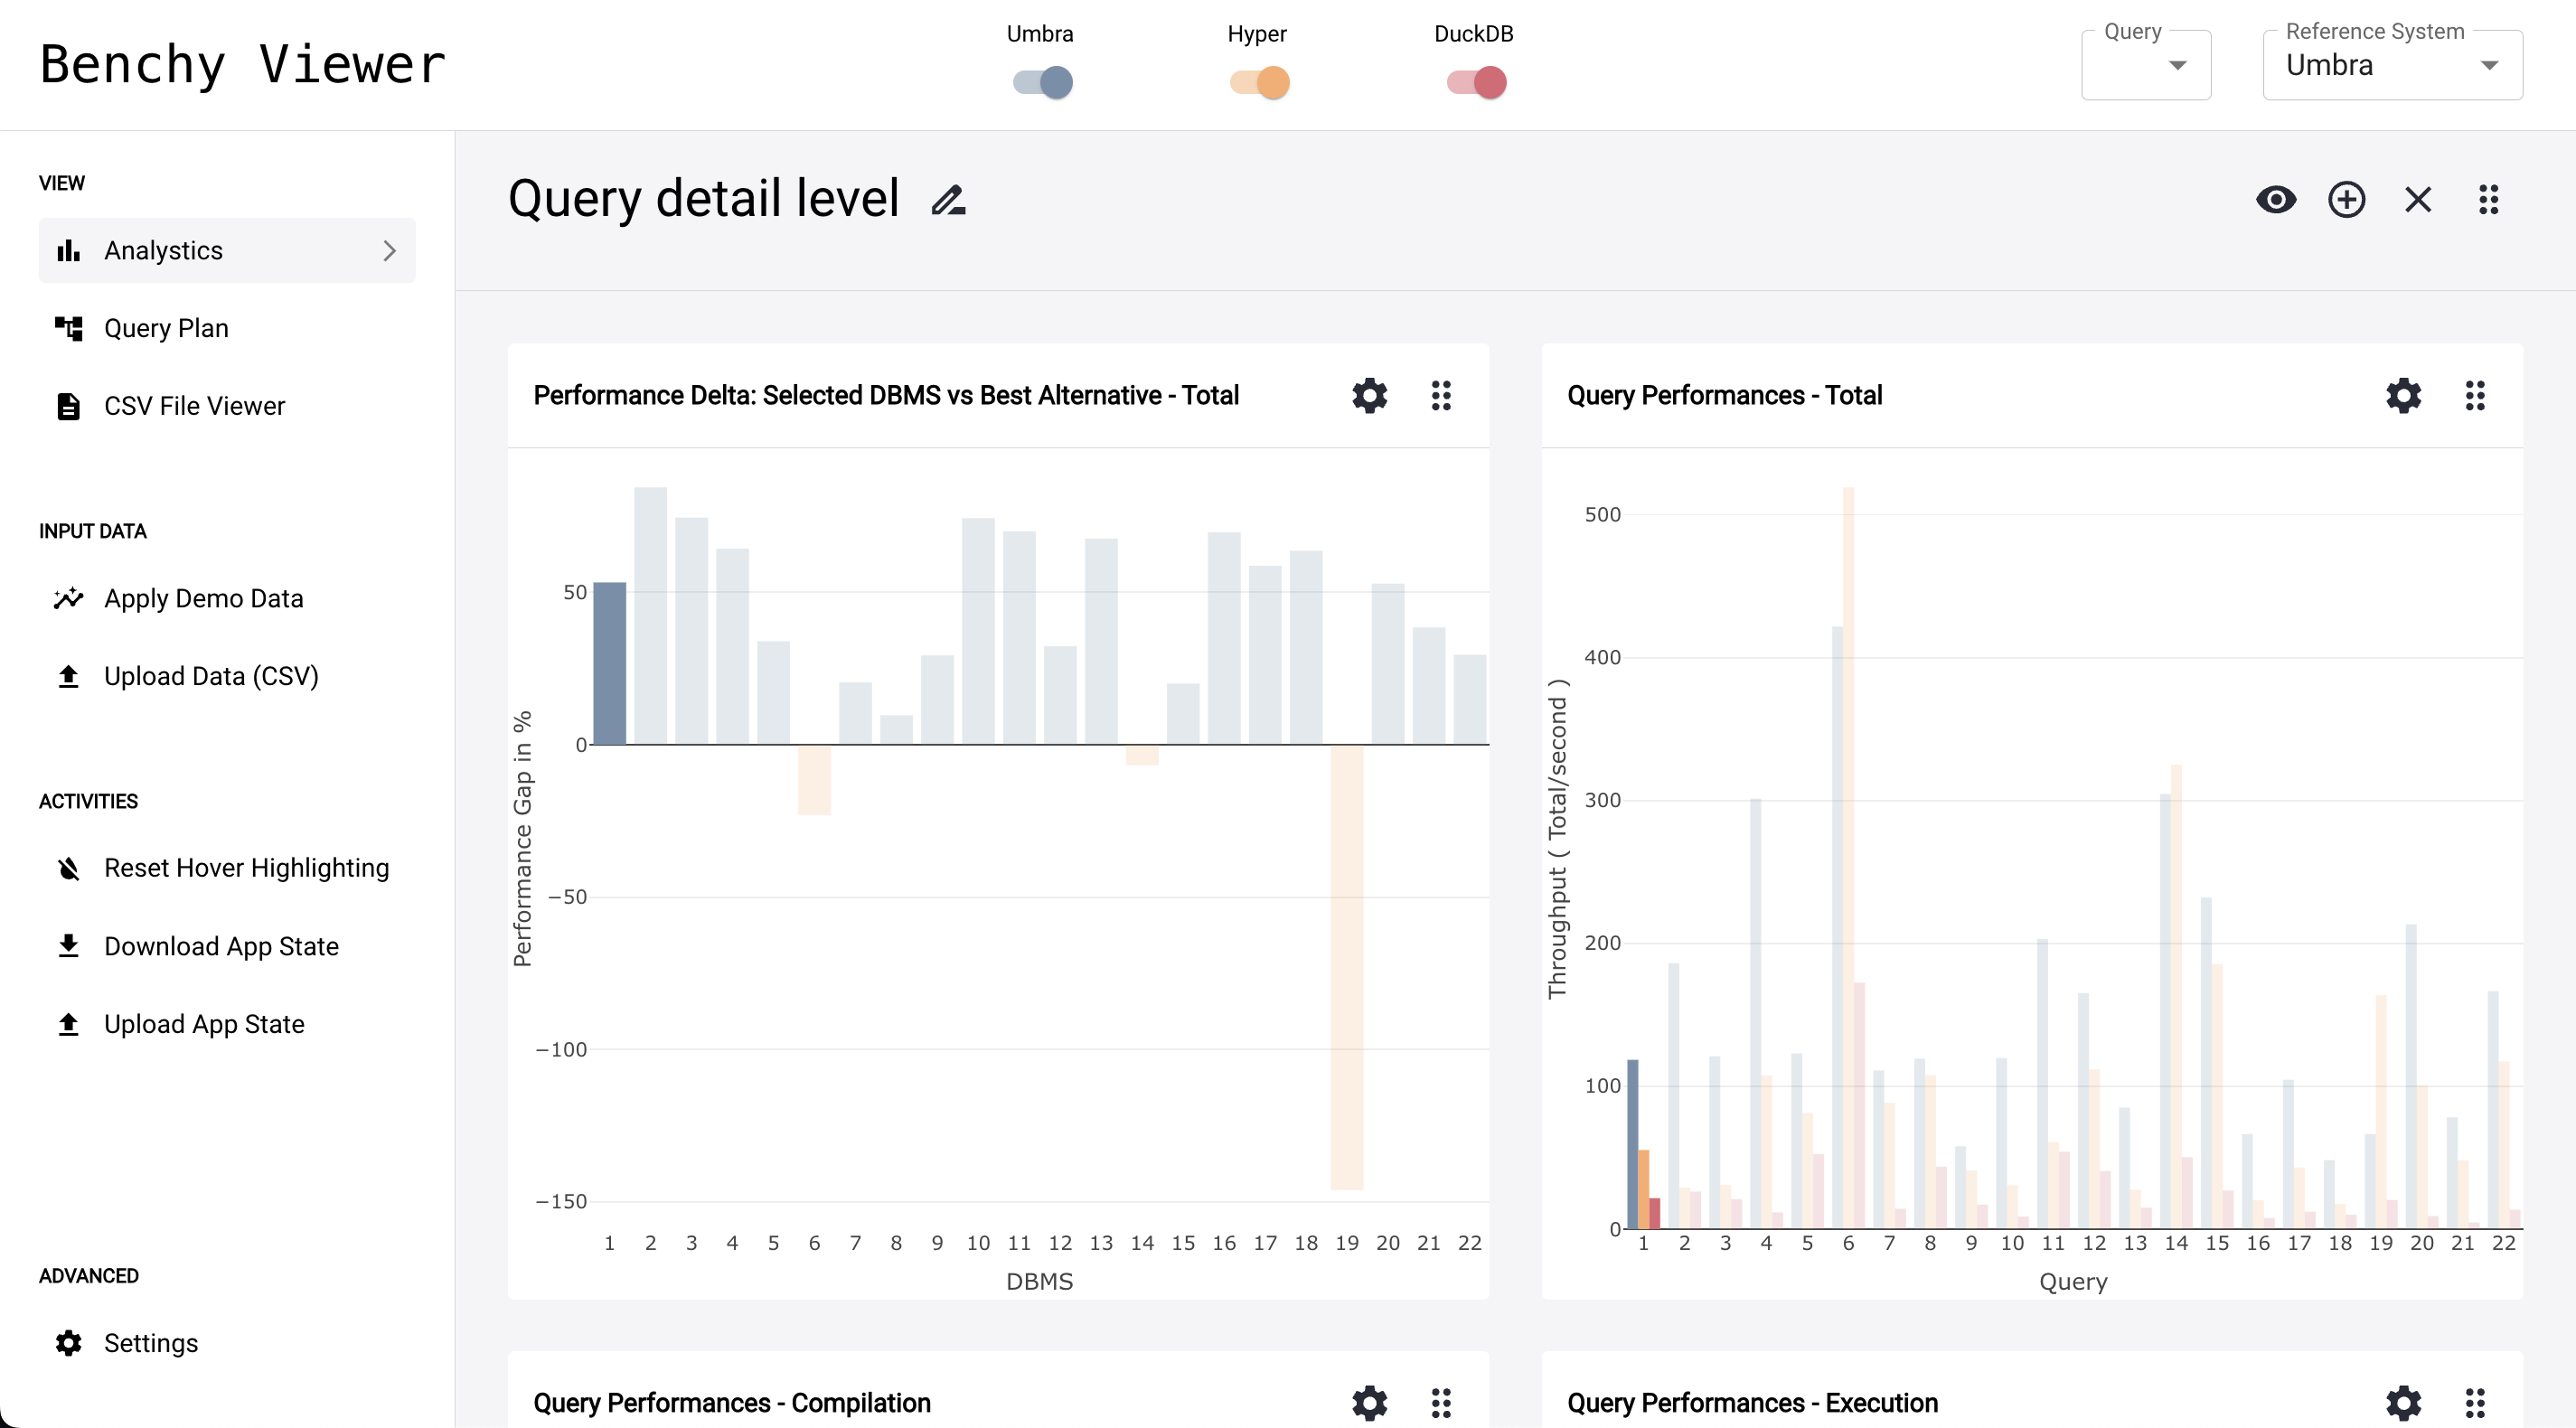
\includegraphics[width=\linewidth]{figures/app.png}
    \caption{Analytics dashboard.}
      \label{fig:app-page}
  \end{subfigure}
  \hspace{0.5cm} % Adjust the horizontal space between the figures
  \begin{subfigure}[b]{0.3\linewidth}
    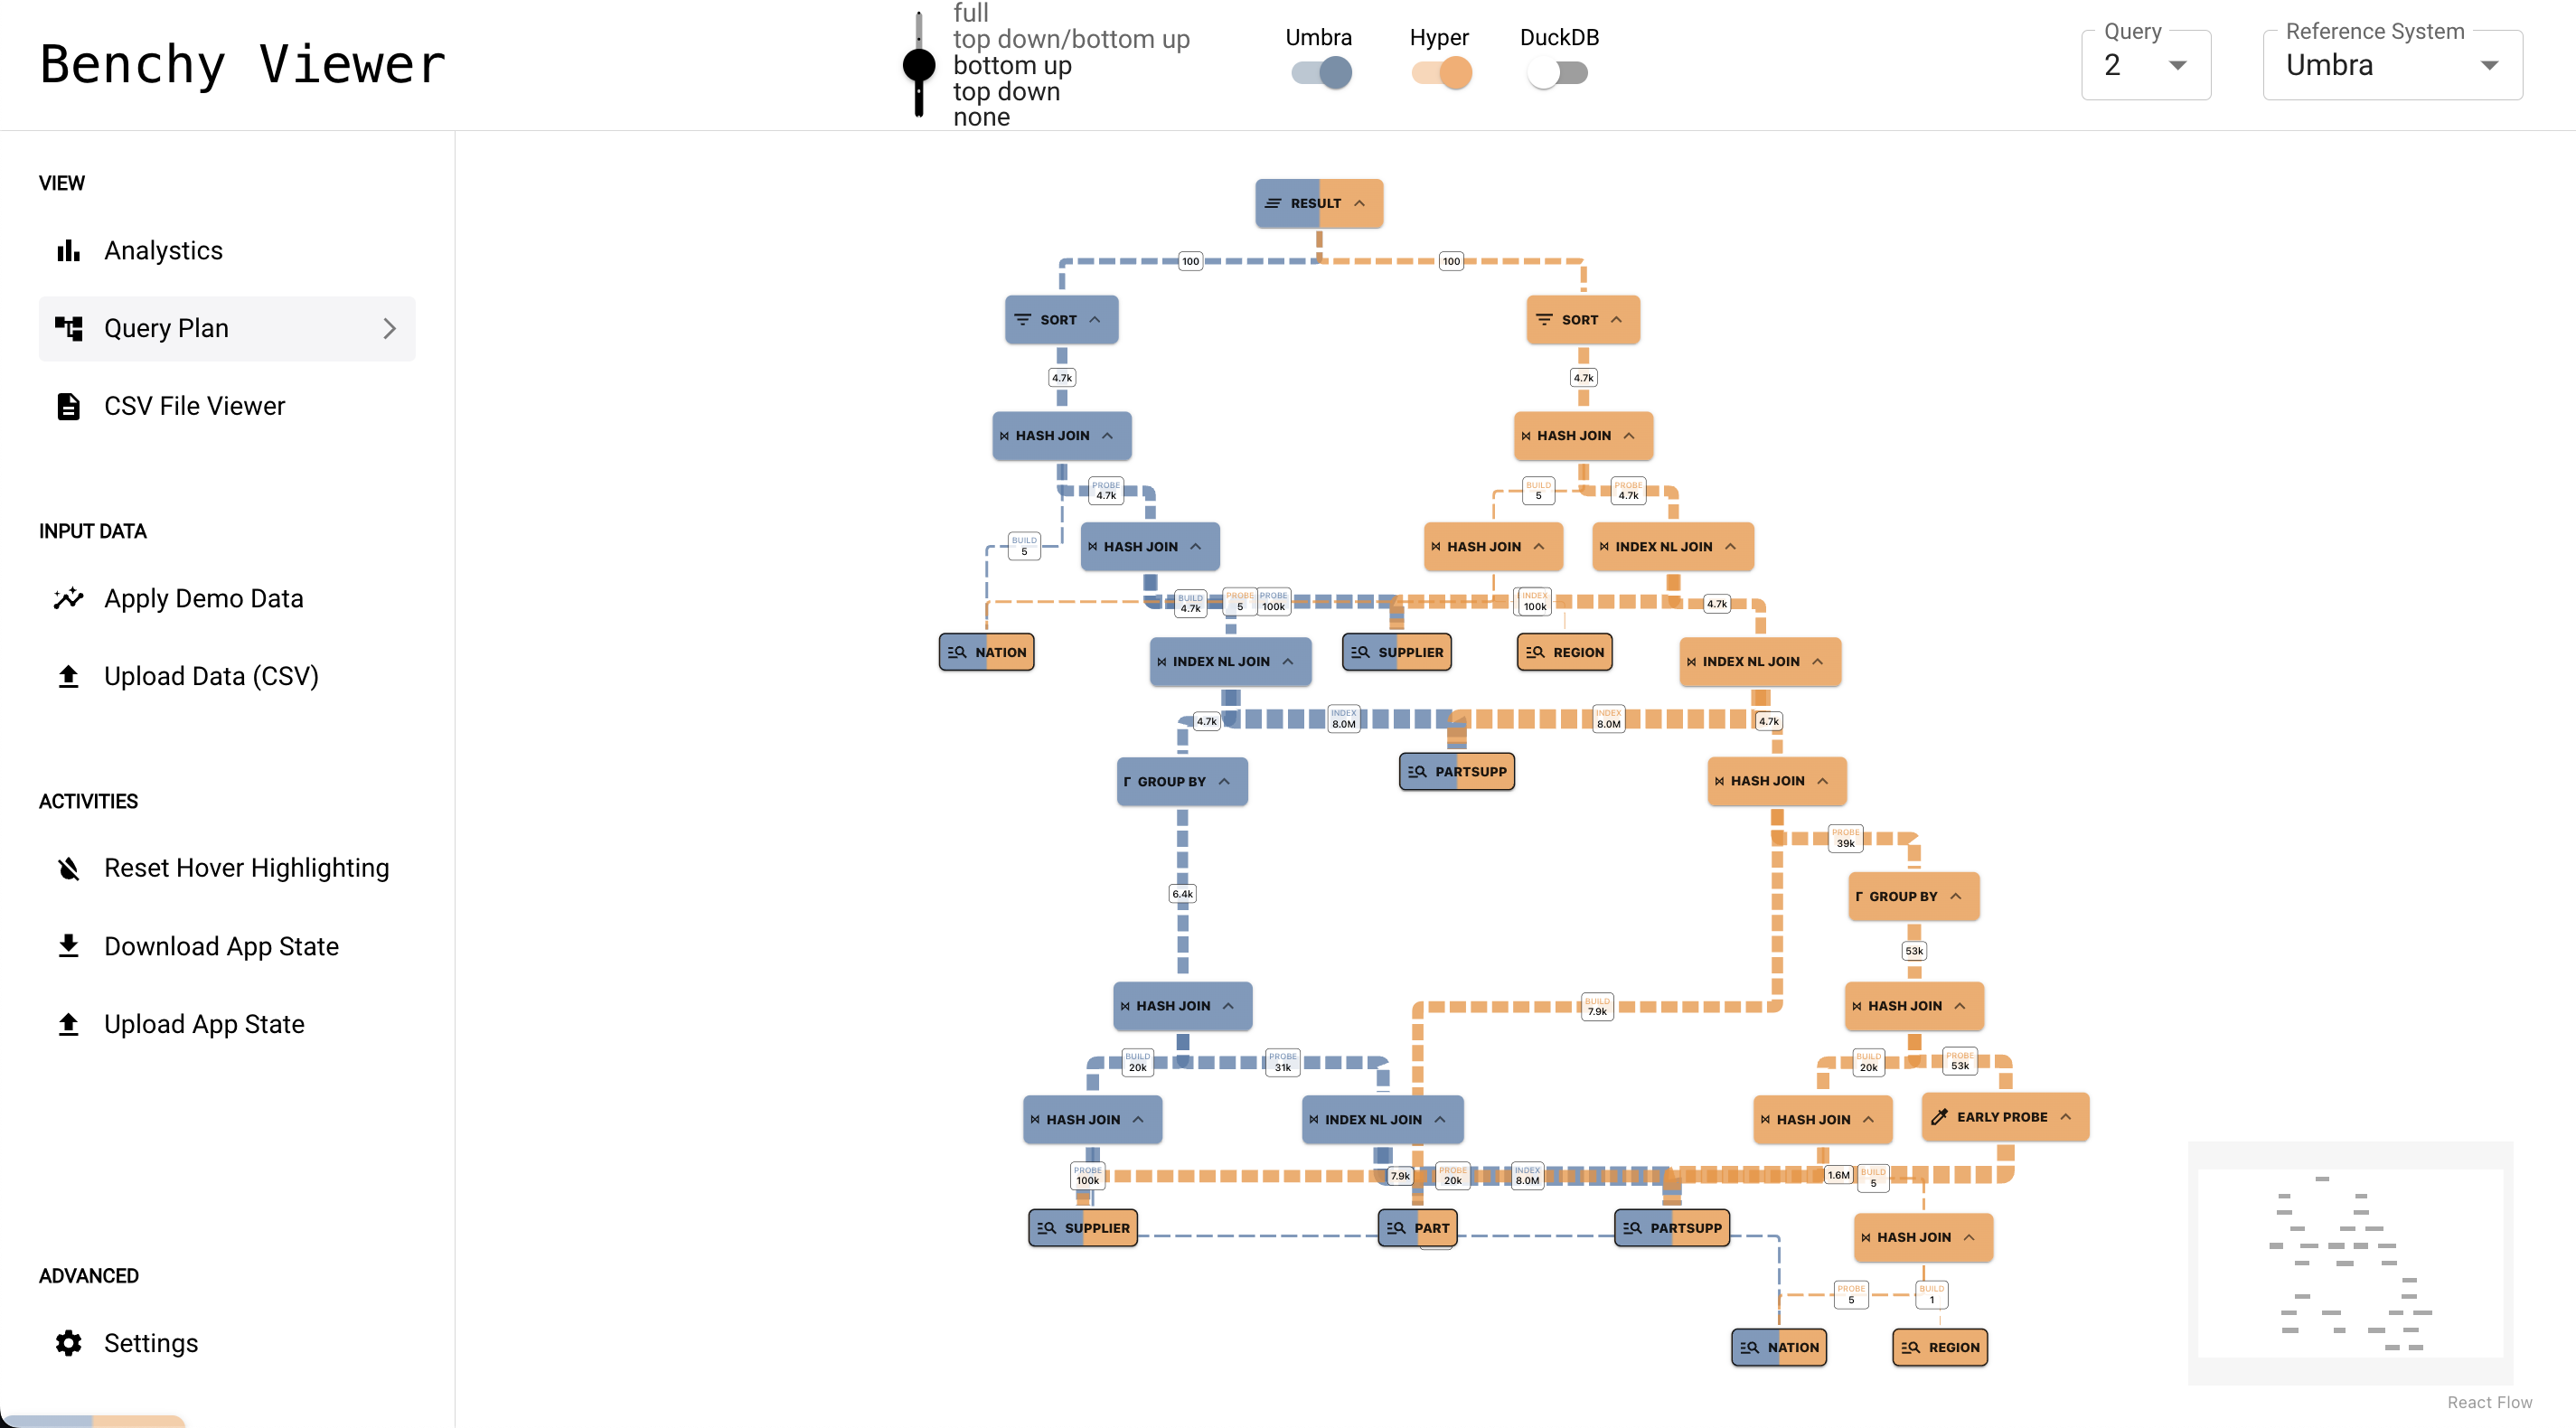
\includegraphics[width=\linewidth]{figures/app-query-plan.png}
    \caption{Query plan view.}
      \label{fig:app-query-plan}
  \end{subfigure}
  \hspace{0.5cm} % Adjust the horizontal space between the figures
  \begin{subfigure}[b]{0.3\linewidth}
    \includegraphics[width=\linewidth]{figures/app-data-viewer.png}
    \caption{Input file viewer.}
      \label{fig:app-data-viewer}
  \end{subfigure}
  \caption{From left to right: Analytics dashboard page, query plan page, and input file viewer page}
  \label{fig:pages}
\end{figure}

The Analytics Dashboard page features the drag-and-drop system for visualising elements and their containers. This page serves as the hub for analysing benchmark data, offering charts and plots to explore queries from diverse perspectives.

Upon identifying significant queries using the analytics dashboard, users often transition to the Query Plan page. This page serves as a central hub for comparing distinct query plans across various database systems. 

In contrast, the Input File Viewer page offers a minimalist perspective. Tailored for users seeking an unembellished view of their imported benchmark data, this page omits visualizations. It provides an in-depth examination of the raw data, enabling users to scrutinize the dataset's structure and intricacies without the influence of charts or plots.















\section{Data Structure}
Unraveling the complexities of the Benchy Viewer necessitates a deep dive into its fundamental data structure, a cornerstone shaping the app's functionality and user interaction.\\
Our exploration commences with an examination of the broad project data structure, leading to a comprehensive exploration of each intricate facet of this structural canvas.

\subsection{Overall Project Structure}

The Benchy Viewer embodies a robust project structure that leverages React, global state management, and a page navigating router, as illustrated in Figure \ref{fig:project-structure}, which we will explore in this section.

\begin{figure}[h]
  \vspace{0.5cm}
  \centering
  \includegraphics[width=0.5\linewidth]{figures/project-structure.png}
  \caption{Project Structure Hierarchy}
  \label{fig:project-structure}
\end{figure}

\subsubsection{Root Component}
The root component is the entry point of the Benchy Viewer React application, orchestrating critical processes that define its robustness and efficiency.\\
The primary responsibility of the root component is to render the main application, serving as the nexus for various functionalities, providing the structural and organizational backbone for the entire application. 

In the project structure hierarchy, the root component encapsulates the application with\texttt{ <React.StrictMode/>}~\parencite{reactstrictmode}, which is a tool that highlights common issues and potential problems in a React application during development.
In general, it detects impure calculations in the context of component states and multiple rendering. It enables a set of additional checks and warnings to catch and alert developers about unsafe or deprecated practices, contributing to better code quality. While it doesn't affect the production build, it's a valuable aid in identifying and addressing issues early in the development phase.


\subsubsection{State Management with Redux}
The Redux Provider in the Benchy Viewer, built using the Redux~Framework~\parencite{Redux}, serves as the central hub for managing the application's state. It acts as a shared space where different parts of the application can store and retrieve data efficiently.\\
Utilizing the capabilities of \textit{Redux Toolkit}\parencite{redux-toolkit}, the Redux Provider supplies the global state across the entire application. This global state is compartmentalized into five distinct slices, illustrated in Figure~\ref{fig:global-state}, each serving a unique purpose.

\begin{figure}[h]
  \centering
  \includegraphics[width=0.8\linewidth]{figures/global-state.png}
  \caption{Application State Compartements}
  \label{fig:global-state}
\end{figure}

% Analytics Dashboard state
The Analytics Dashboard State encapsulates all the data concerning visualizations within the Analytics Dashboard. It includes information about the position within the dashboard and the configuration of each visualization element. A more detailed exploration of this data structure is provided in Section \ref{sec:analytics-dashboard}.

% Imported Benchmark Data state
The Current Benchmark Data State is responsible for holding all benchmark data from various database systems. This state is a pivotal component used across the Analytics Dashboard, Query Plan View, and Benchmark Data View. A detailed examination of this state's structure is available in Section \ref{sec:input-data}.

% Global Settings state
Focused on interactive features within visualizations, the Global Settings State encompasses functionalities like the global hover state or the selected query. Section \ref{sec:global-settings} delves into the specifics of this data structure.

% Query Plan Parameters state
Tailoring the visualization needs for the user, the Query Plan Parameters State contains data related to the appearance and comparison types of the query plans. More insights into this state are provided in Section \ref{sec:query-plan-parameters}.

% Query Plan Nodes state
Lastly, the Query Plan Nodes State unfolds the story of the actual query plan, housing details about every node and their associated information. For a comprehensive exploration, turn to Section \ref{sec:query-plan-structure}.


\subsubsection{Router}
Navigating through the corridors of the Benchy Viewer's project structure, the router, powered by \textit{React Router} \parencite{react-router}, providing a standardized approach to handle navigation in React. Specifically, in our application, this router guides users through three key areas: the Analytics Dashboard, Query Plan View, and Data Viewer.

\subsubsection{Layout and Content}
Finally, we encounter the pages with their contents within the Benchy Viewer. These pages share a consistent structure, ensuring a unified user experience. Each page adheres to a standardized layout, featuring a sidebar, a header, and a dedicated space for content, which we discussed the page structure in \ref{sec:page-structure}.

At this point, the various components at different levels come together to form the Benchy Viewer application. The root component lays the groundwork, overseeing essential processes. The Redux Provider acts as a central hub for sharing information across the application. The global state, divided into five slices, provides state to all pages. The router facilitates easy navigation between pages, which is controlled in the sidebar. In essence, these pages, with their structured layouts, unite to offer users a seamless and comprehensive experience.














\subsection{Benchmark Data}\label{sec:input-data}

The initial step when engaging with the Benchy Viewer involves importing a file containing performance data slated for visualization. This file must adhere to the format outlined in Section \ref{sec:input-file-structure} and is processed by the Current Benchmark Data State, introduced in the previous section. 

\subsubsection{Import Process}

Throughout the importation process, the input file undergoes parsing and transformation into a TypeScript object. Subsequently, the benchmark data is partitioned according to the respective database systems. This partitioning ensures that all query data aligns with its associated database system. The resulting data structure encompasses a system ID, a title, all pertinent benchmark data, and an activation flag.

\subsubsection{Data Accessibility}

After the data import, the benchmark data is accessible to all visualization elements across the whole Benchy Viewer. This includes all visualization elements within the Analytics Dashboard, the File Viewer, and the Query Plan View.

The activation flag controls the visibility of the system data of a whole database system in the visualizations. This is accessed through the header's legend toggles, where users can control the activation or deactivation of database systems.

Additionally, this state holds the demo data, which is initialised on the start of the application. Upon user requests via the sidebar, the demo data is loaded as the current benchmark data.



\subsection{Global Settings}\label{sec:global-settings}

In the Benchy Viewer, the Global Settings serve as a central hub for interactive and customizable data exploration. Features like hover and selected queries offer real-time insights, while selecting a baseline system deepens understanding for comparative analysis. Visual configurations provide the power to mould data representation, aligning with user preferences. In essence, the Global Settings act as the control center, empowering users for dynamic and tailored data exploration.

\subsubsection{Hovered Query}

A key interactive feature is the global hover functionality, where details about the currently hovered query are stored. This information is triggered when a user hovers over a specific query within a visualization element on a detailed level, like a bar in a bar chart. This hover information is then synchronized across all other visualizations simultaneously.

\subsubsection{Selected Query}

Much like the hover feature, the selected query is stored and activated through interactions within the visualization elements at a detailed level. Additionally, a drop-down input in the header allows users to manually select the current query. This state is utilized not only for highlighting purposes in the Analytics Dashboard, but also in the Query Plan View for selecting the corresponding query plan.

\subsubsection{Baseline System}

Another crucial component within this data slice is the selected baseline system, a linchpin for comparative analyses in the Benchy Viewer. This feature empowers users to delve into the results of their chosen system, comparing and contrasting its performance against other systems. This is particularly valuable in visualizations incorporating metrics like speed-up and slow-down.

Specifically utilized in visualizations such as the comparative query bar chart, the selected baseline system plays a vital role in illustrating the performance delta for each query. This allows users to discern the nuanced differences between the baseline system and the best-performing alternative. 

\subsubsection{Visualization Configurations}

This segment houses configuration options influencing the visual aspects of charts, detailed in Section \ref{sec:chart-configuration}. It governs factors like the chart axis scale and display type for violin plots. Users can conveniently access and tweak these options through the settings menu in the sidebar. The choices made here resonate across various visualization elements in the Analytics Dashboard, providing a tailored and cohesive visual experience.










\subsection{Analytics Dashboard Data Structure}\label{sec:analytics-dashboard}

The Analytics Dashboard in the Benchy Viewer acts as a central hub for comprehensive performance analysis, providing a structured and user-friendly interface. At its core, the data structure slice forms the backbone, storing essential information about analytics sections and the visual elements they contain.

\subsubsection{Containers}
This data slice manages a roster of analytics sections, with their order mirroring the sequence in the UI's drag-and-drop system. Reordering the analytics sections in the UI through the drag-and-drop feature will update this state.

Each container in the list retains a name for labeling the analytics section. Additionally, a visibility flag dictates whether the container is collapsed or its content, along with all its charts, is visible. In general, all of these properties are accessible in the UI through the containers header.\\
Lastly, every container holds a list of its associated visualization elements. 

\subsubsection{Visualization Element}
Within each container, a list of visualization elements is stored, aligning with the sequence in the UI's drag-and-drop system. Reordering charts in the UI through the drag-and-drop feature will update this state.

These visualization elements are distinguished by a label in their header, signifying their content.\\
Furthermore, each element is characterized by a property denoting its visual type, such as a bar chart or violin plot.\\
Lastly, a vital attribute is the metric associated with each visualization element, ranging from execution time to compilation time. In the UI, this is accessible through the chart menu, see \ref{sec:chart-configuration}.





\subsection{Query Plan}
The incorporation of the query plan into the Benchy Viewer relies heavily on the integration of the Query Plan Visualizer \parencite{semantic-diff}. For a more detailed exploration of this integration, refer to Section \ref{sec:semantic-diff-integration}.

The query plan's data structure is divided into two essential parts. First, there are parameters governing the visual aspects and comparison strategies of the query plans. Second, we have the actual query plan data for the database systems.

\subsubsection{Visualization Parameters}\label{sec:query-plan-parameters}

To enhance the user experience, the Query Plan Viewer incorporates a collapsible functionality in every node, denoted by an icon. Recognizing that some users may find this feature unnecessary, an option exists in the settings to disable collapsibility. This choice hides all icons in the nodes, ensuring a cleaner and less distracting look for the query plan.

The matching algorithm parameter is a pivotal component influencing the visualization of query plans in the Benchy Viewer. This property, structured as an enum, provides a spectrum of options to tailor the matching algorithm based on specific visualization needs. It is accessible in the header when the Query Plan View is active, as depicted in Figure~\ref{fig:query-plan-slider}. When set to "none", it allows query plans to be displayed independently, side by side, without any comparison. Alternatively, choosing "top down" or "bottom up" initiates matching algorithms that prioritize either a top-down or bottom-up approach, optimizing clarity in specific scenarios. The "top down/bottom up" option combines both methods, offering a balanced approach.

Lastly, users have the option to customize the visualization of edges within the query plan. By default, edges are presented in horizontal and vertical directions, reminiscent of a classical tournament tree. However, when dealing with intricate query plans or non-planar graphs, overlapping edges may compromise clarity. To address this, users can modify the edge style. This customization allows edges to deviate from strict horizontal or vertical orientations, adopting a more dynamic style that allocates additional space to each edge. This flexibility ensures that the visual representation of edges aligns with the structure of the query plans, contributing to a more informative visualization.



\subsubsection{Query Plan Data Structure}\label{sec:query-plan-structure}

During the import of benchmark data into the Benchy Viewer, the query plan metadata undergoes a transformation process to populate a structured object. This involves parsing the raw metadata provided in the benchmark results, which includes details such as the operator ID, estimated cardinality, and exact cardinality.

The data transformation involves creating instances that represent each element of the query plan, forming a tree structure to reflect the hierarchical arrangement. This establishes relationships between elements to capture the flow and nesting of operations. System-specific details are retained within each node throughout this transformation. This structured representation enables users to navigate the intricacies of the query execution flow.








\section{Integration of Plotly-React for Data Visualization}
\subsection{Types of Plots and Charts}
\subsection{Hover Feature}
\subsection{Selected Query Feature}

\section{Integration of semantic-diff-tool}\label{sec:semantic-diff-integration}
\subsection{Business Logic}
\subsection{Settings}
\subsection{UI}
% !TeX root = ../main.tex
% Add the above to each chapter to make compiling the PDF easier in some editors.

\chapter{Discussion}\label{chapter:discussion}

\section{Evaluation of Achievement of Objectives}

\section{Critical Reflection on the App Development}
\subsection{Challenges/ Technical Limitations (Performance limits)}
\subsection{Design Choices and Trade-offs}
\subsection{Comparison with Existing Solutions}
\subsection{Potentials and Future Improvements}
% !TeX root = ../main.tex
% Add the above to each chapter to make compiling the PDF easier in some editors.

\chapter{Conclusion}\label{chapter:conclusion}

\section{Summary of Results}
\section{Future Developments and Enhancements}

% !TeX root = ../main.tex
% Add the above to each chapter to make compiling the PDF easier in some editors.

\chapter{Example}\label{chapter:example}

\section{Section}
Citation test~\parencite{latex}.

Acronyms must be added in \texttt{main.tex} and are referenced using macros. The first occurrence is automatically replaced with the long version of the acronym, while all subsequent usages use the abbreviation.

E.g. \texttt{\textbackslash ac\{TUM\}, \textbackslash ac\{TUM\}} $\Rightarrow$ \ac{TUM}, \ac{TUM}

For more details, see the documentation of the \texttt{acronym} package\footnote{\url{https://ctan.org/pkg/acronym}}.
\subsection{Subsection}

See~\autoref{tab:sample}, \autoref{fig:sample-drawing}, \autoref{fig:sample-plot}, \autoref{fig:sample-listing}.

\begin{table}[htpb]
  \caption[Example table]{An example for a simple table.}\label{tab:sample}
  \centering
  \begin{tabular}{l l l l}
    \toprule
      A & B & C & D \\
    \midrule
      1 & 2 & 1 & 2 \\
      2 & 3 & 2 & 3 \\
    \bottomrule
  \end{tabular}
\end{table}

\begin{figure}[htpb]
  \centering
  % This should probably go into a file in figures/
  \begin{tikzpicture}[node distance=3cm]
    \node (R0) {$R_1$};
    \node (R1) [right of=R0] {$R_2$};
    \node (R2) [below of=R1] {$R_4$};
    \node (R3) [below of=R0] {$R_3$};
    \node (R4) [right of=R1] {$R_5$};

    \path[every node]
      (R0) edge (R1)
      (R0) edge (R3)
      (R3) edge (R2)
      (R2) edge (R1)
      (R1) edge (R4);
  \end{tikzpicture}
  \caption[Example drawing]{An example for a simple drawing.}\label{fig:sample-drawing}
\end{figure}

\begin{figure}[htpb]
  \centering

  \pgfplotstableset{col sep=&, row sep=\\}
  % This should probably go into a file in data/
  \pgfplotstableread{
    a & b    \\
    1 & 1000 \\
    2 & 1500 \\
    3 & 1600 \\
  }\exampleA
  \pgfplotstableread{
    a & b    \\
    1 & 1200 \\
    2 & 800 \\
    3 & 1400 \\
  }\exampleB
  % This should probably go into a file in figures/
  \begin{tikzpicture}
    \begin{axis}[
        ymin=0,
        legend style={legend pos=south east},
        grid,
        thick,
        ylabel=Y,
        xlabel=X
      ]
      \addplot table[x=a, y=b]{\exampleA};
      \addlegendentry{Example A};
      \addplot table[x=a, y=b]{\exampleB};
      \addlegendentry{Example B};
    \end{axis}
  \end{tikzpicture}
  \caption[Example plot]{An example for a simple plot.}\label{fig:sample-plot}
\end{figure}

\begin{figure}[htpb]
  \centering
  \begin{tabular}{c}
  \begin{lstlisting}[language=SQL]
    SELECT * FROM tbl WHERE tbl.str = "str"
  \end{lstlisting}
  \end{tabular}
  \caption[Example listing]{An example for a source code listing.}\label{fig:sample-listing}
\end{figure}


\appendix{}

\microtypesetup{protrusion=false}

\addchap{Abbreviations}
\begin{acronym}
	\itemsep-.25\baselineskip
	\acro{TUM}[TUM]{Technical University of Munich}
	% TODO: add acronyms
\end{acronym}

\listoffigures{}
\listoftables{}
\microtypesetup{protrusion=true}
\printbibliography{}

\end{document}
